\documentclass[
	ngerman,
	ruledheaders=section,%Ebene bis zu der die Überschriften mit Linien abgetrennt werden, vgl. DEMO-TUDaPub
	class=report,% Basisdokumentenklasse. Wählt die Korrespondierende KOMA-Script Klasse
	thesis={type=master},% Dokumententyp Thesis
	accentcolor=2c, % Akzentfarbe FG rtm
	custommargins=false,
	marginpar=false,
	BCOR=10mm, % Bindekorrektur (etwas größere mittlere Ränder)
	parskip=half-, % Absatzkennzeichnung durch Abstand vgl. KOMA-Sript
	fontsize=11pt, % Basisschriftgröße laut Corporate Design ist mit 9pt häufig zu klein
  	twoside,
  	numbers=noendperiod,
  	fleqn,
  	captions=oneline, % Einzeilige Captions zentrieren
	captions=tableheading, % Für besseren Abstand bei TabellenÜBERschriften
  	IMRAD=false,
]{tudapub}


%%%%%%%%%%%%%%%%%%%
%Pakete einbinden
%%%%%%%%%%%%%%%%%%%
%%%%%%%%%%%%%%%%%%%
% Mathe-Umgebungen und Symbole
%%%%%%%%%%%%%%%%%%%
\usepackage{amsmath}
\usepackage{amssymb}

%%%%%%%%%%%%%%%%%%%
% TikZ für Blockschaltbilder und Skizzen
%%%%%%%%%%%%%%%%%%%
\usepackage{tikz}				% Zum Erzeugen von Bildern mit TikZ
% TikZstyles-Bibliothek f�r Blockschaltbilder

\usetikzlibrary{arrows}		
\usetikzlibrary{arrows.meta}
\usetikzlibrary{positioning}

\newcommand{\TikZscale}{1}
\newcommand{\mm}{*\TikZscale mm}
\tikzset{every picture/.style={node distance=4\mm, >=stealth'}}

%% Bl�cke
	% Rechteckige Bl�cke
	\tikzstyle{block}      = [draw, semithick, rectangle, minimum height=8\mm, minimum width=8\mm, inner sep=3pt]
	\tikzstyle{NLblock}    = [draw, semithick, rectangle, minimum height=8\mm, minimum width=8\mm, inner sep=3pt, double distance=1.2pt]
	\tikzstyle{PICblock}   = [draw, semithick, rectangle, minimum height=8\mm, minimum width=8\mm, inner sep=2pt]
	\tikzstyle{NLPICblock} = [draw, semithick, rectangle, minimum height=8\mm, minimum width=8\mm, inner sep=3pt, double distance=1.2pt]
	\tikzstyle{noblock}	   = [rectangle, inner sep=-0.6pt]

	% Dreieckige Bl�cke
	\tikzstyle{Rgain}			 = [draw, semithick, isosceles triangle, inner sep=1pt, minimum height=8\mm, isosceles triangle apex angle=60]
	\tikzstyle{Lgain}			 = [draw, semithick, isosceles triangle, inner sep=1pt, minimum height=8\mm, isosceles triangle apex angle=60, shape border rotate=180]
	\tikzstyle{Ugain}			 = [draw, semithick, isosceles triangle, inner sep=1pt, minimum height=8\mm, isosceles triangle apex angle=60, shape border rotate=90]
	\tikzstyle{Dgain}			 = [draw, semithick, isosceles triangle, inner sep=1pt, minimum height=8\mm, isosceles triangle apex angle=60, shape border rotate=-90]

	% Runde Bl�cke
	\tikzstyle{sum}   	   = [draw, semithick, circle, inner sep=1pt, minimum size=3\mm]
	\tikzstyle{branch}		 = [draw, circle, inner sep=0pt, minimum size=1\mm, fill=black]
	\tikzstyle{BRANCH}		 = [coordinate]


%% Verbindungselemente
	% Linien mit Pfeil
	\tikzstyle{to}  		= [->, thick]
	\tikzstyle{toNL}		= [->, thick, shorten >=0.9pt]
	\tikzstyle{NLto}		= [->, thick, shorten <=0.9pt]
	\tikzstyle{NLtoNL}	= [->, thick, shorten <=0.9pt, shorten >=0.9pt]
	
	\tikzstyle{TO}  		= [semithick, double distance=2pt, shorten >=2mm, decoration={markings,mark=at position 1 with {\arrow[semithick]{open triangle 60}}}, preaction={decorate},postaction={draw, line width=2pt, white, shorten >= 1.5mm}]
	
	\tikzstyle{TONL}  		= [semithick, double distance=2pt, shorten >=2.2mm, decoration={markings,mark=at position 1 with {\arrow[semithick]{open triangle 60}}, transform={xshift=-0.7pt}}, preaction={decorate},postaction={draw, line width=2pt, white, shorten >= 1.5mm}]
	
	\tikzstyle{NLTO}  		= [semithick, double distance=2pt, shorten <=0.9pt, shorten >=2mm, decoration={markings,mark=at position 1 with {\arrow[semithick]{open triangle 60}}}, preaction={decorate}, postaction={draw, line width=2pt, white, shorten >= 1.5mm}]
	
	\tikzstyle{NLTONL}  		= [semithick, double distance=2pt, shorten <=0.9pt, shorten >=2.2mm, decoration={markings,mark=at position 1 with {\arrow[semithick]{open triangle 60}}}, preaction={decorate},postaction={draw, line width=2pt, white, shorten >= 1.5mm}]
	
	\tikzstyle{innerWhite} = [semithick, white,line width=2pt, shorten >= 2mm, shorten <= 2mm]
	
	%\tikzstyle{TO}  		= [semithick, double distance=2pt, shorten >=2mm, decoration={markings,mark=at position 1 with {\arrow[semithick]{open triangle 60}}}, postaction={decorate}]
		%
	%\tikzstyle{TONL} = [semithick, double distance=2pt, shorten >=2.2mm, decoration={markings,mark=at position 1 with {\arrow[semithick]{open triangle 60}}, transform={xshift=-0.7pt}}, postaction={decorate}]
	%
	%\tikzstyle{NLTO} = [semithick, double distance=2pt, shorten <=0.79pt, shorten >=2mm, decoration={markings,mark=at position 1 with {\arrow[semithick]{open triangle 60}}}, postaction={decorate}]
	%
	%\tikzstyle{NLTONL} = [semithick, double distance=2pt, shorten <=0.79pt, shorten >=2.2mm, decoration={markings,mark=at position 1 with {\arrow[semithick]{open triangle 60}}, transform={xshift=-0.7pt}}, postaction={decorate}]
	

	% Linien ohne Pfeil 
	\tikzstyle{line}       = [thick]
	\tikzstyle{lineNL}     = [thick, shorten >= 0.6pt]
	\tikzstyle{NLline}     = [thick, shorten <= 0.6pt]
	\tikzstyle{NLlineNL}	 = [thick, shorten <= 0.6pt, shorten >= 0.6pt]
	
	% Doppellinien ohne Pfeil
	\tikzstyle{LINE}       = [semithick, double distance=2pt]
	\tikzstyle{LINENL}     = [semithick, double distance=2pt, shorten >= 0.9pt]
	\tikzstyle{NLLINE}     = [semithick, double distance=2pt, shorten <= 0.9pt]
	\tikzstyle{NLLINENL}	 = [semithick, double distance=2pt, shorten <= 0.9pt, shorten >= 0.9pt]
	
	\tikzstyle{neg}				 = [postaction={decorate,decoration={markings, mark=at position 1 with{\draw[-](-2pt,-3pt)--(-2pt,-7pt);}}}]
	
	\tikzstyle{labelabove} = [above, anchor=base, yshift=0.75ex]
	\tikzstyle{labelbelow} = [below, anchor=base, yshift=-2ex]
	\tikzstyle{labelright} = [right]
	\tikzstyle{labelleft}  = [left]
	
	
	% Pins und Labels
	\tikzstyle{every pin edge}	= [<-, thick]
	\tikzstyle{every pin}	 			= [pin distance=5\mm]
	\tikzstyle{every label}			= [font=\small]
	\tikzstyle{terminal}				= [coordinate]
	
	% extra Symbole f�r circuits-Library
	\tikzstyle{jack}	= [draw, circle, minimum size=1.5mm, inner sep=0]
 % rtm-eigene Bibliothek für Blockschaltbilder

%%%%%%%%%%%%%%%%%%%
% Plotten direkt in LaTeX
%%%%%%%%%%%%%%%%%%%
\usepackage{pgfplots}

%%%%%%%%%%%%%%%%%%%
% Bilder und Abbildungen
%%%%%%%%%%%%%%%%%%%
\usepackage{pdfpages}
\usepackage{graphicx}
\usepackage{caption}
\usepackage{subcaption}
\usepackage{float}
\usepackage{import}
\usepackage{color}
\usepackage{transparent}


%%%%%%%%%%%%%%%%%%%
%Sprachanpassung & Verbesserte Trennregeln
%%%%%%%%%%%%%%%%%%%
%\usepackage{acronym}
\usepackage[acronym]{glossaries}
\setacronymstyle{long-short}
%\usepackage{glossaries-extra}
\usepackage[english, main=ngerman]{babel}
\usepackage[autostyle]{csquotes}% Anführungszeichen vereinfacht
\usepackage{microtype}
\usepackage{etoolbox}


%%%%%%%%%%%%%%%%%%%
%Meine Makros einbinden
%%%%%%%%%%%%%%%%%%%
\newcommand{\eqp}{\ensuremath{\, \, \, .}}
\newcommand{\M}[1]{\textbf{#1}} %Matrix  M
\newcommand{\Mr}[1]{\textbf{#1}_\rho} %Matrix mit tiefgestelltem rho, M_rho
\newcommand{\Mtil}[1]{\tilde{\textbf{#1}}} %Matrix mit Tilde
\newcommand{\Mtilt}[2]{\tilde{\textbf{#1}}_{#2}} %Matrix mit Tilde mit tiefgestelltem arg2
\DeclareRobustCommand{\Mt}[2]{\textbf{#1}_{#2}} %Matrix M mit tiefgestelltem arg2


\DeclareRobustCommand{\w}[1]{\underline{#1}} %Vektor arg1 unterstrichen 
\DeclareRobustCommand{\wt}[2]{\underline{#1}_{#2}} %Vektor unterstrichen w mit tiefgestelltem arg2
\DeclareRobustCommand{\wr}[1]{\underline{#1}_{\rho}} %Vektor unterstrichen mit rho, w_rho

% Textbausteine
% =============
	% Produktnamen
	\newcommand*{\Matlab}{\textsc{Matlab}}
	\newcommand*{\Matlabreg}{\textsc{Matlab}\textsuperscript{\tiny \textregistered}}
	\newcommand*{\MatSim}{\textsc{Matlab/Simulink}}
	\newcommand*{\Simulink}{\textsc{Simulink}}
	\newcommand*{\Simulinkreg}{\textsc{Simulink}\textsuperscript{\tiny \textregistered}}

	% Das Makro |\name|\marg{person} formatiert einen Personennamen bspw. eines Erfinders oder Entdeckers gemäß |\name{Euler}| \arrow\ \name{Euler}.
	\newcommand*{\name}[1]{\textsc{#1}}
	\newcommand*{\GenderPl}[1]{{#1}\_innen}
	\newcommand*{\GendeSin}[1]{{#1}\_in}
% Makros für Einheiten, Exponenten
% ================================

	\newcommand*{\unit}[1]{\ensuremath{\mathrm{#1}}}
	
	% Wert mit Einheit (mit kleinem Leerzeichen dazwischen), aus Text- UND Math-Modus
	\newcommand*{\valunit}[2]{\ensuremath{#1\,\mrm{#2}}}
	
	
	% "°C", im Text- oder Mathe-Modus
	\newcommand*{\degC}{
		\ifmmode
		^\circ \mrm{C}%
		\else
		\textdegree C%
		\fi}
	
	\newcommand*{\degree}{
		\ifmmode
		^\circ%
		\else
		\textdegree%
		\fi}
	
	% Für Exponentenschreibweise ( Anwendung: 123\E{3} )
	\newcommand*{\E}[1]{\ensuremath{\cdot 10^{#1}}}
	
	\newcommand*{\eexp}[1]{\ensuremath{\mathrm{e}^{#1}}}
	\newcommand*{\iu}{\ensuremath{\mathrm{j}}}
	
	\newcommand*{\todots}{\ensuremath{,\,\hdots,\,}}

% Makros für Formeln
% ==================

	% Definition für Vektor und Matizen
	\newcommand*{\mat}[1]{{\ensuremath{\boldsymbol{\mathrm{#1}}}}}
	\newcommand*{\ma}[1]{{\ensuremath{\boldsymbol{\mathrm{#1}}}}}
	\newcommand*{\mas}[1]{\ensuremath{\boldsymbol{#1}}}
	\newcommand*{\ve}[1]{\ensuremath{\boldsymbol{#1}}}
	\newcommand*{\ves}[1]{\ensuremath{\boldsymbol{\mathrm{#1}}}}
	
	\newcommand*{\AP}{\ensuremath{\mathrm{AP}}}
	\newcommand*{\doti}{\ensuremath{(i)^\cdot}}
	
	\newcommand*{\inprod}[2]{\ensuremath{\langle #1,\,#2 \rangle}}
	
	\newcommand*{\ul}[1]{\underline{#1}}
	
	% gerades "d" (z.B. für Integral)
	\newcommand*{\ud}{\ensuremath{\mathrm{d}}}
	
	% normaler Text in Formeln
	\newcommand*{\tn}[1]{\textnormal{#1}}
	
	% nicht-kursive Schrift in Formeln
	\newcommand*{\mrm}[1]{\ensuremath{\mathrm{#1}}}
	
	% gerades "T" für Transponiert
	\newcommand*{\transp}{\ensuremath{\mathrm{T}}}
	
	% gerades "rg"
	\newcommand*{\rang}{\ensuremath{\operatorname{rg}}}
	
	% Für geklammerte Ausdrücke mit Index (Subscript)
	% (einmal mit kursiven Index, einmal mit geradem Index)
	\newcommand*{\grpsb}[2]{\ensuremath{\left(#1\right)_{#2}}}
	\newcommand*{\grprsb}[2]{\ensuremath{\left(#1\right)_{\mathrm{#2}}}}
	
	% Ableitungen und Integrale
		% "normale" Ableitung (mit geraden "d"s)
		\newcommand*{\normd}[2]{\ensuremath{\frac{\mathrm{d}#1}{\mathrm{d}#2}}}
		\newcommand*{\normdat}[3]{\ensuremath{\left.\frac{\mathrm{d} #1}{\mathrm{d} #2}\right|_{#3}}}
		
		% Materielle Ableitung
		\newcommand*{\matd}[2]{\ensuremath{\frac{\mathrm{D} #1}{\mathrm{D} #2}}}
		\newcommand*{\matdat}[3]{\ensuremath{\left.\frac{\mathrm{D} #1}{\mathrm{D} #2}\right|_{#3}}}
		
		% Partielle Ableitung
		\newcommand*{\partiald}[2]{\ensuremath{\frac{\partial #1}{\partial #2}}}
		\newcommand*{\partialdat}[3]{\ensuremath{\left.\frac{\partial #1}{\partial #2}\right|_{#3}}}
	
	
	% Transformationen
	\newcommand*{\FT}[1]{\ensuremath{\mathfrak{F}\left\{#1\right\}}}
	\newcommand*{\FTabs}[1]{\ensuremath{\left|\mathfrak{F}\left\{#1\right\}\right|}}
	\newcommand*{\IFT}[1]{\ensuremath{\mathfrak{F}^{-1}\left\{#1\right\}}}
	\newcommand*{\DFT}[1]{\ensuremath{\mathrm{DFT}\left\{#1\right\}}}
	\newcommand*{\DFTabs}[1]{\ensuremath{\left|\mathrm{DFT}\left\{#1\right\}\right|}}
	\newcommand*{\Laplace}[1]{\ensuremath{\mathfrak{L}\left(#1\right)}}
	\newcommand*{\InvLaplace}[1]{\ensuremath{\mathfrak{L^{-1}}\left(#1\right)}}
	\newcommand*{\invtrans}{\ensuremath{\quad\bullet\!\!-\!\!\!-\!\!\circ\quad}}
	\newcommand*{\trans}{\ensuremath{\quad\circ\!\!-\!\!\!-\!\!\bullet\quad}}
	
	
	\newcommand*{\mlfct}[1]{\texttt{#1}}
	\newcommand*{\mlvar}[1]{\texttt{#1}}
	
	
	% Manche textcomp-Zeichen funktionieren mit dem TU-Design nicht, diese können dann mit diesem
	% Befehl gesetzt werden.
	\newcommand*{\textcompstdfont}[1]{{\fontfamily{cmr} \fontseries{m} \fontshape{n} \selectfont #1}}

% Makros für Variablen
% ================================
\newcommand*{\amax}{\ensuremath{a_{\textrm{max}}}}
\newcommand*{\amin}{\ensuremath{a_{\textrm{min}}}}
\newcommand*{\jmax}{\ensuremath{j_{\textrm{max}}}}
\newcommand*{\jmin}{\ensuremath{j_{\textrm{min}}}}
\newcommand*{\opt}[1]{\ensuremath{{#1}^*}}
\newcommand*{\fofx}{\ensuremath{f(\ve{x})}}
\newcommand*{\J}{\ensuremath{J(\ve{x}(t),\ve{u}(t),t)}}
\newcommand*{\Vofxoftf}{\ensuremath{V(\ve{x}(t_f),t_f)}}
\newcommand*{\Vofxoftone}{\ensuremath{\tilde{V}(\ve{x}(t_1),t_1)}}
\newcommand*{\Vofxoftfallgemein}{\ensuremath{\bar{V}(\ve{x}(t_f),t_f)}}
\newcommand*{\Vofxoftoftonefallgemein}{\ensuremath{\hat{V}(\ve{x}(t_f),\ve{x}(t_1),t_f,t_1)}}
\newcommand*{\variation}[1]{\ensuremath{\ve{\delta}_{#1}}}
\newcommand*{\dtint}[1]{\ensuremath{\textrm{d}{#1}}}
% Makros für x(t) Variablen
% ================================
\newcommand*{\xzero}{\ensuremath{\ve{x}_0}}
\newcommand*{\xoft}{\ensuremath{\ve{x}(t)}}
\newcommand*{\xoftf}{\ensuremath{\ve{x}(t_f)}}
\newcommand*{\xoftzero}{\ensuremath{\ve{x}(t_0)}}
\newcommand*{\xoftone}{\ensuremath{\ve{x}(t_1)}}
\newcommand*{\xofti}{\ensuremath{\ve{x}(t_i)}}
\newcommand*{\xoftoneminus}{\ensuremath{\ve{x}(t_1^-)}}
\newcommand*{\xoftoneplus}{\ensuremath{\ve{x}(t_1^+)}}
\newcommand*{\xoptoft}{\ensuremath{\opt{\ve{x}}(t)}}
\newcommand*{\xoptoftf}{\ensuremath{\opt{\ve{x}}(t_f)}}
\newcommand*{\xoptoftzero}{\ensuremath{\opt{\ve{x}}(t_0)}}
\newcommand*{\xoptoftfopt}{\ensuremath{\opt{\ve{x}}(\opt{t_f})}}
% Makros für x(tau) Variablen
% ================================
\newcommand*{\xoftau}{\ensuremath{\ve{x}(\tau)}}
\newcommand*{\xoftauf}{\ensuremath{\ve{x}(\tau_f)}}
\newcommand*{\xoftauzero}{\ensuremath{\ve{x}(\tau_0)}}
\newcommand*{\xoptoftau}{\ensuremath{\opt{\ve{x}}(t\tau)}}
\newcommand*{\xoptoftauf}{\ensuremath{\opt{\ve{x}}(\tau_f)}}
\newcommand*{\xoptoftauzero}{\ensuremath{\opt{\ve{x}}(\tau_0)}}
\newcommand*{\xoptoftaufopt}{\ensuremath{\opt{\ve{x}}(\opt{\tau_f})}}
% Makros für dx(t) Variablen
% ================================
\newcommand*{\dx}{\ensuremath{\dot{\ve{x}}}}
\newcommand*{\dxoft}{\ensuremath{\dot{\ve{x}}(t)}}
\newcommand*{\dxoftf}{\ensuremath{\dot{\ve{x}}(t_f)}}
\newcommand*{\dxoftzero}{\ensuremath{\dot{\ve{x}}(t_0)}}
\newcommand*{\dxoptoft}{\ensuremath{\dot{\ve{x}}^*(t)}}
\newcommand*{\dxoptoftf}{\ensuremath{\dot{\ve{x}}^*(t_f)}}
\newcommand*{\dxoptoftfopt}{\ensuremath{\dot{\ve{x}}^*(\opt{t_f})}}
% Makros für dx(tau) Variablen
% ================================
\newcommand*{\dxoftau}{\ensuremath{\ve{x}'(\tau)}}
\newcommand*{\dxoftauf}{\ensuremath{\ve{x}'(\tau_f)}}
\newcommand*{\dxoftauzero}{\ensuremath{\ve{x}'(\tau_0)}}
\newcommand*{\dxoptoftau}{\ensuremath{\ve{x}'^*(\tau)}}
\newcommand*{\dxoptoftauf}{\ensuremath{\ve{x}'^*(\tau_f)}}
\newcommand*{\dxoptoftaufopt}{\ensuremath{\ve{x}'^*(\opt{\tau_f})}}
% Makros für u(t) Variablen
% ================================
\newcommand*{\uoft}{\ensuremath{\ve{u}(t)}}
\newcommand*{\uoftf}{\ensuremath{\ve{u}(t_f)}}
\newcommand*{\uoftzero}{\ensuremath{\ve{u}(t_0)}}
\newcommand*{\uoptoft}{\ensuremath{\opt{\ve{u}}(t)}}
\newcommand*{\uoptoftf}{\ensuremath{\opt{\ve{u}}(t_f)}}
\newcommand*{\uoptoftfopt}{\ensuremath{\opt{\ve{u}}(\opt{t_f})}}
% Makros für u(tau) Variablen
% ================================
\newcommand*{\uoftau}{\ensuremath{\ve{u}(\tau)}}
\newcommand*{\uoftauf}{\ensuremath{\ve{u}(\tau_f)}}
\newcommand*{\uoftauzero}{\ensuremath{\ve{u}(\tau_0)}}
\newcommand*{\uoptoftau}{\ensuremath{\opt{\ve{u}}(\tau)}}
\newcommand*{\uoptoftauf}{\ensuremath{\opt{\ve{u}}(\tau_f)}}
\newcommand*{\uoptoftaufopt}{\ensuremath{\opt{\ve{u}}(\opt{\tau_f})}}
% Makros für lambda(t) Variablen
% ================================
\newcommand*{\lambdaoft}{\ensuremath{\ve{\lambda}(t)}}
\newcommand*{\lambdaoftf}{\ensuremath{\ve{\lambda}(t_f)}}
\newcommand*{\lambdaoftone}{\ensuremath{\ve{\lambda}(t_1)}}
\newcommand*{\lambdaoftzero}{\ensuremath{\ve{\lambda}(t_0)}}
\newcommand*{\lambdaoftoneminus}{\ensuremath{\ve{\lambda}(t_1^-)}}
\newcommand*{\lambdaoftoneplus}{\ensuremath{\ve{\lambda}(t_1^+)}}
% Makros für lambda(tau) Variablen
% ================================
\newcommand*{\lambdaoftau}{\ensuremath{\ve{\lambda}(\tau)}}
\newcommand*{\lambdaoftauf}{\ensuremath{\ve{\lambda}(\tau_f)}}
% Makros für dlambda(t) Variablen
% ================================
\newcommand*{\dlambda}{\ensuremath{\dot{\ve{\lambda}}}}
\newcommand*{\dlambdaoft}{\ensuremath{\dot{\ve{\lambda}}(t)}}
% Makros für dlambda(tau) Variablen
% ================================
\newcommand*{\dlambdaoftau}{\ensuremath{\ve{\lambda}'(\tau)}}
% Makros für z(t) Variablen
% ================================
\newcommand*{\zzero}{\ensuremath{\ve{z}_0}}
\newcommand*{\zoft}{\ensuremath{\ve{z}(t)}}
\newcommand*{\zoftf}{\ensuremath{\ve{z}(t_f)}}
\newcommand*{\zoftzero}{\ensuremath{\ve{z}(t_0)}}
\newcommand*{\zoptoft}{\ensuremath{\opt{\ve{z}}(t)}}
\newcommand*{\zoptoftf}{\ensuremath{\opt{\ve{z}}(t_f)}}
\newcommand*{\zoptoftzero}{\ensuremath{\opt{\ve{z}}(t_0)}}
\newcommand*{\zoptoftfopt}{\ensuremath{\opt{\ve{z}}(\opt{t_f})}}
% Makros für z(tau) Variablen
% ================================
\newcommand*{\zoftau}{\ensuremath{\ve{z}(\tau)}}
\newcommand*{\zoftauf}{\ensuremath{\ve{z}(\tau_f)}}
\newcommand*{\zoftauzero}{\ensuremath{\ve{z}(\tau_0)}}
\newcommand*{\zoptoftau}{\ensuremath{\opt{\ve{z}}(\tau)}}
\newcommand*{\zoptoftauf}{\ensuremath{\opt{\ve{z}}(\tau_f)}}
\newcommand*{\zoptoftauzero}{\ensuremath{\opt{\ve{z}}(\tau_0)}}
\newcommand*{\zoptoftaufopt}{\ensuremath{\opt{\ve{z}}(\opt{\tau_f})}}
% Makros für dz(t) Variablen
% ================================
\newcommand*{\dz}{\ensuremath{\dot{\ve{z}}}}
\newcommand*{\dzoft}{\ensuremath{\dot{\ve{z}}(t)}}
\newcommand*{\dzoftf}{\ensuremath{\dot{\ve{z}}(t_f)}}
\newcommand*{\dzoftzero}{\ensuremath{\dot{\ve{z}}(t_0)}}
\newcommand*{\dzoptoft}{\ensuremath{\dot{\ve{z}}^*(t)}}
\newcommand*{\dzoptoftf}{\ensuremath{\dot{\ve{z}}^*(t_f)}}
\newcommand*{\dzoptoftfopt}{\ensuremath{\dot{\ve{z}}^*(\opt{t_f})}}
% Makros für dz(tau) Variablen
% ================================
\newcommand*{\dzoftau}{\ensuremath{\ve{z}'(\tau)}}
\newcommand*{\dzoftauf}{\ensuremath{\ve{z}'(\tau_f)}}
\newcommand*{\dzoftauzero}{\ensuremath{\ve{z}'(\tau_0)}}
\newcommand*{\dzoptoftau}{\ensuremath{\ve{z}'^*(\tau)}}
\newcommand*{\dzoptoftauf}{\ensuremath{\ve{z}'^*(\tau_f)}}
\newcommand*{\dzoptoftaufopt}{\ensuremath{\ve{z}'^*(\opt{\tau_f})}}
% Makros für Ttransformation Variablen
% ================================
\newcommand*{\Ttransoftau}{\ensuremath{\mathcal{T}(\tau)}}
\newcommand*{\Ttransoftauzero}{\ensuremath{\mathcal{T}(\tau_0)}}
\newcommand*{\Ttransoftauf}{\ensuremath{\mathcal{T}(\tau_f)}}
% Makros für dTtransformation Variablen
% ================================
\newcommand*{\dTtransoftau}{\ensuremath{\mathcal{T}'(\tau)}}
\newcommand*{\dTtransoftauzero}{\ensuremath{\mathcal{T}'(\tau_0)}}
\newcommand*{\dTtransoftauf}{\ensuremath{\mathcal{T}'(\tau_f)}}



%%%%%%%%%%%%%%%%%%%
%Literaturverzeichnis
%%%%%%%%%%%%%%%%%%%
\catcode30=12  % Workaround for current biblatex problem (https://tex.stackexchange.com/questions/564990/error-after-miktex-reinstall-text-line-contains-an-invalid-character)
\usepackage[backend=biber,style=ieee,bibencoding=utf8]{biblatex}
\addbibresource{./Bib/literature.bib}

% ======================================================
% Fix für Fehlermeldungen 'Undifined control sequence' und 'Missing number, treated as zero.' bei gestapelten Akzenten in der Mathe-Umgebung. (z.B. \dot{\hat{x}})
% Der Fehler tritt auf bei tuda-ci v3.10 (Feb. 2021) in Kombination mit dem amsmath package.
%
% BITTE PRÜFEN, OB DER FEHLER NOCH BESTEHT UND DEN WORKAROUND GGF. WIEDER ENTFERNEN
%
% workaround/solution by skillmon posted here
% https://tex.stackexchange.com/questions/482281/math-accent-symbol-over-parentheses-enclosing-accented-symbol-amsmath
\makeatletter
\protected\def\mathaccentV#1#2#3#4#5%
  {%
    \ifmmode
      \mathaccentV@do{#2}{#3}{#4}{#5}%
    \else
      \@xp\nonmatherr@\csname #1\endcsname
    \fi
  }
\def\mathaccentV@do#1#2#3#4%
  {%
    \global\let\macc@nucleus\@empty
    \mathaccent"\accentclass@#1#2#3{#4}\macc@nucleus
  }
\makeatother
% ======================================================

\makeglossaries


%\newacronym{FAS}{FAS}{Fahrerassistenzsysteme}
%\newacronym{ACC}{ACC}{Adaptive Cruise Control}
%\newacronym{FSRA}{FSRA}{Full Speed Range Adaptive Cruise Control}
%\newacronym{FSW}{FSW}{Fahrstreifenwechsel}
\newglossaryentry{FAS}{name=FAS,description={Fahrassistenzsystem}}
\newglossaryentry{ACC}{name=ACC,description={Adaptive Cruise Control}}
\newglossaryentry{FSRA}{name=FSRA,description={Full Speed Range Adaptive Cruise Control}}
\newglossaryentry{FSW}{name=FSW,description={Fahrstreifenwechsel}}
\newglossaryentry{LKS}{name=LKS,description={Lane Keeping Support}}
\setcounter{secnumdepth}{3}
\setcounter{tocdepth}{3}
\begin{document}
% =================================================================================
% Header mit allen Metadaten etc. 
% =================================================================================
\Metadata{	% Metadaten im erzeugten PDF/A
	title=Masterthesis Markus Amann,
	author=Markus Amann,
	keywords={TU Darmstadt \sep Corporate Design \sep LaTeX},
}

\title{Trajektorienplanung als dynamisches Optimalsteuerungsproblem und Interpretation des Lösungsraums für Fahrkomfort im automatisierten Fahren}
\subtitle{\textmd{Studiengang Elektrotechnik und Informationstechnik}}
\author[Markus Amann]{Markus Amann}
\reviewer*[Erstprüfer,Betreuer]{Prof. Dr.-Ing. Ulrich Konigorski \and Wi Mi M.Sc. Alexander Steinke} % erst ab Version v3.06 (2020-10-20) des tuda-ci-Pakets möglich

\department{etit}

\addTitleBox{
\includegraphics[width=\linewidth]{Bilder/rtm_mit_schrift}}

%\date{\today}
\submissiondate{4. Juli 2022}

\lowertitleback{
	Technische Universität Darmstadt\\
	Institut für Automatisierungstechnik und Mechatronik\\
	Fachgebiet Regelungstechnik und Mechatronik\\
	Prof. Dr.-Ing. Ulrich Konigorski\\
}

\frontmatter
\maketitle

\clearpage
\setcounter{page}{1}
\section*{Aufgabenstellung}

%\documentclass[
%	paper=a4,
%	ngerman,
%	accentcolor=2c, % Akzentfarbe FG rtm
%	type=announcement,
%	marginpar=false,
%	fleqn,
%	class=report,
%	fontsize=11pt
%	]{tudaposter}
%
%%%%%%%%%%%%%%%%%%%%
%%Sprachanpassung & Verbesserte Trennregeln
%%%%%%%%%%%%%%%%%%%%
%\usepackage[english, main=ngerman]{babel}
%\usepackage[autostyle]{csquotes}% Anführungszeichen vereinfacht
%\usepackage{microtype}
%
%\usepackage{amsmath,amssymb}
%
%\usepackage{url}
%
%%%%%%%%%%%%%%%%%%%%
%%Literaturverzeichnis
%%%%%%%%%%%%%%%%%%%%
%\catcode30=12  % Workaround for current biblatex problem (https://tex.stackexchange.com/questions/564990/error-after-miktex-reinstall-text-line-contains-an-invalid-character)
%\usepackage[backend=biber,style=ieee,bibencoding=utf8]{biblatex}
%%\addbibresource{model_fidelity.bib}
%
%\renewcommand*{\bibfont}{\small}
%\newcommand{\un}[1]{\, \text{#1}}
%\newcommand{\ve}[1]{\mathbf{#1}}
%\newcommand{\veG}[1]{\text{\boldmath{$#1$}}}
%
%\begin{document}
%
%\title{Trajektorienplanung als dynamisches Optimalsteuerungsproblem und Interpretation des Lösungsraums für Fahrkomfort im automatisierten Fahren \vspace{0.2cm}}
%\subtitle{Aufgabenstellung zur Masterthesis}
%\titleinfo{Betreuer: Alexander Steinke, M.Sc.\\ \today}
%\addTitleBox{
\includegraphics[width=\linewidth]{rtm_mit_schrift}}
%
%\maketitle
%%\section*{Aufgabenbeschreibung}
%
%%Zum numerischen Lösen Dynamischer Optimierungsprobleme können direkte und indirekt
%
%%Ein häufiger Ansatz zum Lösen dynamische Optimierungsprobleme ist die 
%
%%Dynamische Optimierungsprobleme lassen sich analytisch (Dynamische Optimierung) oder numerisch (Statische Optimierung) lösen. Während in der statischen Optimierung

Die allgemeine Struktur eines Optimalsteuerungsproblems lautet
%
\begin{equation*} \begin{aligned}
		\min\limits_{\ve{u}(t)} \ \ \ & J(\ve{u})=V(\ve{x}(t_\text{f}),t_\text{f}) + \int_{t_0}^{t_\text{f}}l(\ve{x}(t),\ve{u}(t),t)\text{d}t \\
		\text{u.B.v.} \ \ \ & \dot{\ve{x}}(t)=\ve{f}(\ve{x}(t),\ve{u}(t),t), \ \ve{x}(t_0)=\ve{x}_0\\ 
		& \mathbf{g}(\ve{x}(t_\text{f}),t_\text{f}) = \ve{0} \\
		& \mathbf{h}(\ve{x}(t),\ve{u}(t),t) \leq \ve{0}.
\end{aligned} \end{equation*}
%
Häufig werden dynamische Optimierungsprobleme (OP) mithilfe direkter Verfahren numerisch gelöst. 
In diesem Fall wird das dynamische in ein statisches OP überführt und der endliche Lösungsvektor $\ve{u}_\text{opt} \in \mathcal{U} \subseteq \mathbb{R}^m$ berechnet. 
Direkte Verfahren haben den Vorteil, dass Zustandsbeschränkungen leichter berücksichtigt werden können und der Konvergenzbereich größer ist. 
Indirekte Verfahren hingegen liefern eine Einsicht in die Struktur der optimalen Lösung.

In der dynamischen Optimierung hingegen werden Funktionen $\ve{u}(t)$ einer unabhängigen Variable $t$ gesucht. 
Mithilfe der Variationsrechnung können Optimalitätsbedingungen hergeleitet werden, die ein Randwertproblem formulieren. 
Die Lösung dieses Randwertproblems liefert in der Folge die optimale Steuertrajektorie $\ve{u}_\text{opt}(t)$. 
Jedoch ist das Lösen des Randwertproblems für nichtlineare Systeme häufig schwierig, weswegen auf numerische Verfahren zurückgegriffen werden muss.

Um im automatisierten Fahren (AD) gezielt Fahrprofile mittels einer optimalen Trajektorienplanung erstellen zu können, ist ein tieferes Verständnis der optimalen Lösung erforderlich. 
Mit einem direkten Verfahren ist die Interpretation der Lösung schwierig, da die Lösung aus reinen Zahlenwerten besteht. 
Zwar könnte ein gewünschtes Fahrverhalten in definierten Fahraufgaben durch zusätzliche Terme im Gütemaß und Anpassung der Gewichte erzielt werden, jedoch ist eine Übertragung auf andere Fahraufgaben fraglich. 
Eine parametrierte Steuertrajektorie $\ve{u}_\text{opt}(t)$ würde die Interpretation erheblich vereinfachen.


Ziele dieser Arbeit sind folgende Punkte:
\begin{enumerate}
	\item Übersicht für Lösungsverfahren dynamischer OPs und Einordnung des AD-Planungsproblems
	\item Erstellen von dynamischen OPs, die durch Variationsrechnung lösbar sind und Lösen dieser
	\begin{enumerate}
		\item Geeignete Fahrszenarien (z.B. Geradeausfahrt, Kurve, Geraden-Kurven-Kombination, Spurwechsel)
		\item Geeignete Komfortmerkmale (z.B. Beschleunigung, Ruck, Fahrdauer)
		\item Berücksichtigung von Begrenzungen
	\end{enumerate}
	\item Interpretation der Lösungenstrajektorien hinsichtlich des dargestellten Funktionenraums 
	\item Einordnung im Kontext Fahrkomfort
\end{enumerate}

Die Ergebnisse sind geeignet zu visualisieren und zu dokumentieren. Die aktuelle Fassung der Richtlinien zur Anfertigung von Abschlussarbeiten ist zu beachten.


%%Technische Universität Darmstadt \\
%%Institut für Automatisierungstechnik und Mechatronik \\
%%Fachgebiet Regelungstechnik und Mechatronik \\
%%Prof. Dr.-Ing. Ulrich Konigorski
%
%%\vspace*{\fill} {\tiny
%%\printbibliography[heading=none]}
%
%\end{document}


\vspace{0.5cm}
\begin{tabular}{ll}
	Beginn: 	& ------ \\
	Ende: 		& ------ \\
	Seminar: 	& ------ \\
\end{tabular}
\clearpage

\affidavit

\section*{Kurzfassung}
Zusammenfassung entsprechend der Dokumentensprache. In diesem Fall Deutsch.
\section*{Abstract}
Additional abstract in English.	

\cleardoublepage

\tableofcontents
\cleardoublepage

\mainmatter


% =================================================================================
% Kapitel und Sections etc.
% =================================================================================
\chapter{Einleitung}\label{cha:Einleitung}

- kurze erklärung was fahrfremde Tätigkeit bedeutet und welche relevanz das für autonomes Fahren hat. 
- kurz ein paar Worte zu Kinetose und Hinweis darauf, dass es später noch genauer erklärt wird
\glsadd{utc}
\chapter{Fahrkomfort und Einordnung in den Kontext Automatisiertes Fahren}\label{cha:Komfort}
In diesem Kapitel soll der Begriff \glqq Fahrkomfort\grqq~in den Kontext \gls{AD} eingeordnet werden. Dazu wird zunächst die Bedeutung des Begriffs genauer betrachtet und die Verbindung zwischen Fahrkomfort und Sicherheitsempfinden dargelegt. Anschließend werden verschiedene Einflussfaktoren auf die Komfortwahrnehmung während des Fahrens thematisiert. Dabei wird das Phänomen der Kinetose genauer erklärt und speziell auf dessen Bedeutsamkeit für die Entwicklung automatisierter Fahrzeuge eingegangen. Abschließend werden mithilfe von Literaturwerten Grenzwerte für die als relevant erachteten Einflüsse untersucht. 
%\section{Begriffsdefinition Komfort}
%Während der Begriff ``Komfort'' im alltäglichen Sprachgebrauch eine sehr vielseitige Bedeutung hat und dabei sowohl zur Beschreibung positiver Empfindungen wie Wohlbehagen und Zufriedenheit, als auch in negierter Form zur Beschreibung negativer Gefühle wie Unwohlsein und Unzufriedenheit verwendet wird, wird bei der wissenschaftlichen Verwendung oftmals stärker differenziert. Es exisitieren verschiedene Modelle, die alle darauf abzielen, eine allgemeine Definition von Komfort zu liefern. Im Sinne der besseren Unterscheidbarkeit und damit einer genaueren Anwendung der entsprechenden Bedeutung, wird häufig zusätzlich der Begriff ``Diskomfort'' verwendet. In \cite{Zhang} wurden in einer Studie Faktoren für das Empfinden von Komfort und Diskomfort beim Sitzen identifiziert, wodurch sich die beiden Begriffe differenzierter verwenden lassen. Während Komfort durch Gefühle, die allgemein als positiv wahrgenommen werden, wie Entspanntheit, Ruhe und Zufriedenheit, klassifiziert wird, zeichnet sich Diskomfort vor allem durch negativ konnotierte Empfindungen, wie Müdigkeit und Rastlosigkeit, aber auch durch biometrische Faktoren, die spürbare Schmerzen verursachen, aus. Die Autoren leiten ein Modell her, in dem Komfort und Diskomfort zwei orthogonale Größen sind, die auch gleichzeitig erfahrbar sind. Während die Abwesenheit von Diskomfort nicht automatisch zur Zunahme von Komfort führt (dasselbe gilt auch anders herum), führt eine Zunahme von Diskomfort zwangsläufig zu einer Abnahme von Komfort. Wie Festner in \cite{Festner_diss} herausarbeitet, ist die Beseitigung von Diskomfort eine notwendige, jedoch nicht hinreichende Bedingung für das Empfinden von Komfort. Da jedoch unangenehme Situationen oftmals deutlicher explizit als solche wahrgenommen werden können, denn angenehme Situationen als angenehm, kann auch der erlebte Diskomfort als Kriterium für den fehlenden Komfort genutzt werden \cite{Festner}. 
%
%Ein weiteres Modell, welches breite Verwendung findet, ist die Komfortpyramide nach Krist \cite{Krist}. 
%\begin{figure}[h]
%	\centering
%	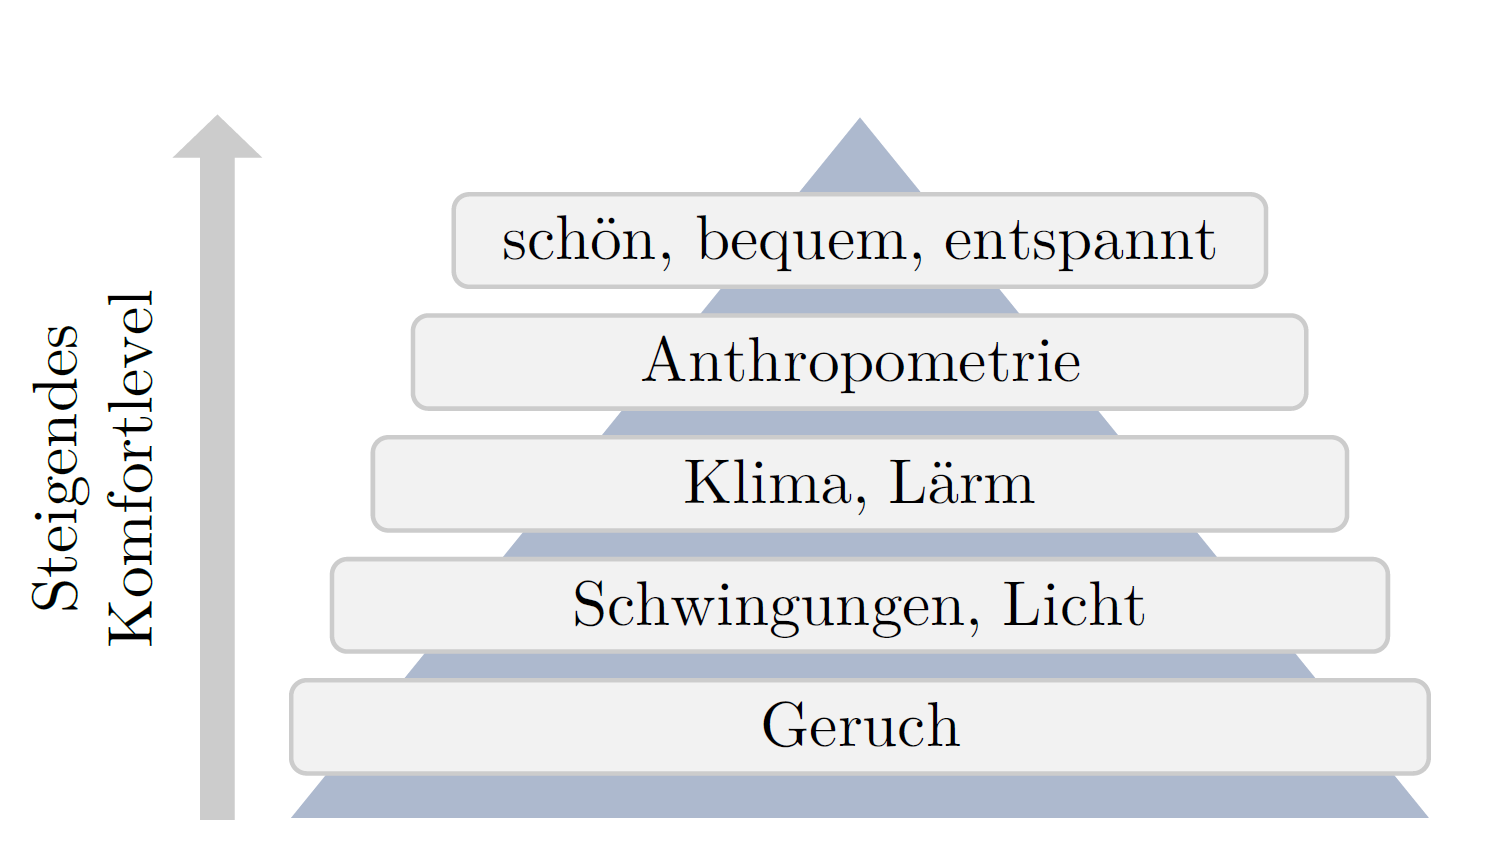
\includegraphics[scale=0.3]{./Bilder/komfortpyramide.png}
%	\label{fig:komfortpyramide}
%	\caption{Komfortpyramide aus \cite{Festner}, zitiert nach \cite{Krist}}
%\end{figure}
%
%In dieser Pyramide nimmt das Komfortlevel, ausgehend von sehr elementaren Faktoren wie Geruch und Lichteinflüssen, stetig zu. Um ein hohes Maß an Komfort zu erzielen, müssen notwendiger Weise zunächst die unteren, grundlegenden Bedingungen erfüllt sein. Zwar werden in diesem Modell Komfort und Diskomfort nicht so streng von einander getrennt, wie in \cite{Zhang}, allerdings ist die Bedingung, dass die Faktoren auf den unteren Ebenen zuerst erfüllt sein müssen damit auch auf den oberen Ebenen die Komfortbedingungen erfüllt werden können, vergleichbar mit der notwendigen Beseitigung von Diskomfort. Neben der qualitativen Beschreibung von Komfort, die alle Modelle gemein haben, unterscheiden sich die Ergebnisse, die unter Verwendung dieser Modelle erzielt werden, dennoch zum Teil stark, da die Komfortwahrnehmung sehr subjektiv ist und sich zwischen einzelnen Personen stark unterscheiden kann. Es lassen sich zwar einzelne Merkmale als komfortabel oder unkomfortabel klassifizieren, allerdings geht aus den Modellen nicht eindeutig hervor, wie stark die einzelnen Merkmale das persönliche Komfortempfinden beeinflussen. Zum Beispiel entwickelt jeder Mensch seine eigene Komfortpyramide, abhängig von ganz persönlichen Faktoren und Erfahrungen \cite{Krist}.
 
\section{Fahrkomfort im Kontext Automatisiertes Fahren}\label{sec:fahrkomfort}
Mit zunehmender Automatisierung von Fahraufgaben rückt auch der Fahrkomfort immer mehr in den Fokus. Es ist nicht davon auszugehen, dass hochautomatisierte oder autonome Fahrzeuge, deren Fahrweise von \GenderPl{Passagier} als unkomfortabel empfunden wird, eine hohe Akzeptanz finden werden. Damit sich überhaupt ein komfortables Gefühl während einer automatisierten Fahrt einstellen kann, muss bei den fahrzeugführenden Personen ein Gefühl von Sicherheit herrschen \cite{Festner.2019}. Nicht nur für unbeteiligte Dritte wie \GenderPl{Fußgänger} oder andere \GenderPl{Autofahrer}, sondern vor allem auch für die fahrzeugführende Person selbst spielt die Sicherheit bei automatisierten Fahrzeugen daher eine zentrale Rolle. In \cite{Festner.2019} wird dabei der Unterschied zwischen subjektiver und objektiver Sicherheit dargelegt. Während das subjektive Sicherheitsempfinden lediglich wiedergibt, wie der Fahrer oder die Fahrerin die Fahrt oder einzelne Situationen empfindet, lässt sich die objektive Sicherheit mithilfe von Größen wie reduzierten Unfallzahlen quantifizieren. Allerdings kann das subjektive Sicherheitsempfinden durchaus von der objektiven Sicherheit abweichen. Insbesondere bei FAS, die nach der SAE-Klassifizierung \cite{SAETaxonomy.2018} Stufe 3 oder höher zugeordnet werden, und bei denen damit das Fahrzeug nicht nur die Längs- und Querführung, sondern zusätzlich auch die Umfeldüberwachung übernimmt, kommt der in \cite{Elbanhawi.2015} als \glqq\textit{loss of controllability}\grqq~eingeführte Paradigmenwechsel von \GendeSin{Fahrer} zu \GendeSin{Passagier} zum Tragen. Dadurch, dass Fahrzeugführende mehr und mehr die Fahrzeugführung und Überwachung aller Funktionen an das Fahrzeug abgeben, stellt sich möglicherweise ein Gefühl von Kontrollverlust ein, weshalb nicht nur die objektive Sicherheit neuartiger Systeme eine große Rolle bei der Bewertung der Systeme spielt, sondern auch das subjektive Sicherheitsempfinden, welches eng an den wahrgenommenen Komfort geknüpft ist. Mit Umfeldüberwachung ist im Sinne der SAE-Klassifizierung die Detektion, Erkennung und Klassifizierung von Objekten im Straßenverkehr sowie Fahrsituationen und die Vorbereitung einer angemessenen Reaktion auf diese gemeint \cite{SAETaxonomy.2018}. Bis einschließlich Level 2 liegt diese Aufgabe bei der fahrzeugführenden Person, während das Fahrzeug nur die eigentliche Quer- und Längsführung ausführt. Ab Level 3 fällt auch diese Aufgabe in den Bereich des Fahrzeugs, sodass das Fahrzeug die dynamische Fahraufgabe vollständig selbst ausüben kann und die fahrzeugführende Person nur noch als Rückfallebene dient und die Fahrzeugführung in Not- oder Fehlersituationen nach Aufforderung durch das System sicher übernehmen kann \cite{SAETaxonomy.2018}.

Neben dem Sicherheitsempfinden gibt es weitere wichtige Faktoren, die den Fahrkomfort beeinflussen. Großen Einfluss auf das Komfortempfinden hat dabei der Fahrstil. In verschiedenen Studien wurden unterschiedliche Fahrstile identifiziert und in verschiedene Klassen unterteilt \cite{Abendroth.2012,Bellem.2016,Murphey.30.03.200902.04.2009}. So variiert zwar die Anzahl und genaue Bezeichnung der einzelnen Klassen zwischen den verschiedenen Studien, jedoch erstreckt sich das Spektrum immer von \glqq langsam\grqq~oder \glqq komfortorientiert\grqq~bis hin zu \glqq dynamisch/sportlich\grqq~oder sogar \glqq aggressiv\grqq. In \cite{Lange.2014} konnte gezeigt werden, dass der Wunsch nach höherem Komfort mit dem Grad der Automatisierung steigt. Ein Grund für diesen Zusammenhang ist unter anderem, dass das Bedürfnis nach Feedback durch die Straße über das Fahrzeug an die fahrende Person mit zunehmender Automatisierung geringer wird. Daher liegt für automatisierte Fahrzeuge im Alltagsgebrauch ein komfortorientierter Fahrstil nahe. 

Um beurteilen zu können, ob ein Fahrstil als komfortabel oder unkomfortabel wahrgenommen wird, muss zunächst geklärt werden, welche Merkmale dabei besonders großen Einfluss auf das Komfortempfinden haben. In \cite{Scherer.2015} wurden in einer Fahrsimulatorstudie die Merkmale Sicherheitsabstand zum Vorderfahrzeug, das Bremsverhalten, die Fahrzeuggeschwindigkeit sowie -beschleunigung, das Spurhalten, Lenken und die Blinkernutzung als die am häufigsten genannten Komfortkriterien identifiziert, wobei die drei ersten Merkmale von über der Hälfte der Teilnehmenden als relevant erachtet wurden. Neben den hier identifizierten Komfortmerkmalen lässt sich auch die Reisezeit als weiteres Kriterium angeben. Bereits in \cite{Oborne.1978} wurde dargelegt, dass \GenderPl{Passagier}, die einer längeren Reisezeit ausgesetzt sind, ein höheres Maß an Komfort benötigen, als bei einer kürzeren Reisezeit. Jeder Passagier und jede Passagierin geht daher einen subjektiven Kompromiss zwischen der erwarteten Reisezeit und dem akzeptierten Niveau an Diskomfort ein. Aufgrund dessen hängen die von der fahrenden Person als komfortabel empfundenen biomechanischen Werte (Geschwindigkeit, Beschleunigung, Ruck) auch von der Reisezeit ab \cite{Festner.2019}.

Eine besondere Gewichtigkeit bei der Trajektorienplanung bezüglich des Fahrkomforts kommt dem Beschleunigungsverhalten zu. In \cite{Bellem.2016} konnte in zwei Studien für verschiedene Fahrmanöver nachgewiesen werden, dass sich Merkmale wie Längs- und Querbeschleunigung sowie der Fahrzeugruck gut dazu eignen, einen komfortablen Fahrstil von anderen Fahrstilen abzugrenzen. Laut \cite{Elbanhawi.2015} ist der häufigste Ansatz zur Optimierung der Fahrzeugbewegungen, die auf die Fahrzeuginsassen wirkenden Kräfte und Rucke zu minimieren. Dass bei der Betrachtung des Beschleunigungsverhaltens jedoch nicht nur die absoluten Werte der Beschleunigung relevant sind, zeigen die Untersuchungen in \cite{Gianna.1996}. Hier konnte festgestellt werden, dass der Mensch bei lateralen Bewegungen insbesondere gegenüber Änderungen der Beschleunigung sehr sensitiv reagiert und diese besonders gut wahrnimmt. In \cite{Dovgan.2013} konnte ein Algorithmus entwickelt werden, der komfortable Fahrstrategien liefert, wobei als zusätzliches Komfortmerkmal der Ruck verwendet wurde. Dieser sollte dazu im Sinne des Fahrkomforts so gering wie möglich sein.

\subsection{Kinetose und ihre Bedeutung für das Autonome Fahren}\label{sec:kinetose}
Kinetose, oftmals auch als Reise- oder Bewegungskrankheit bezeichnet (engl. \textit{Motion Sickness}), beschreibt das Phänomen, dass man sich bei Reisen -- vor allem im Auto, Flugzeug oder auf einem Schiff -- plötzlich unwohl fühlt. Die Symptome reichen dabei von Blässe und leichter Übelkeit, über Schwindel und Kopfschmerzen, bis hin zum Erbrechen \cite{Money.1970}. Es existieren mehrere Theorien für die genauen Ursachen von Kinetose \cite{Money.1970}. Eine anerkannte und weit verbreitete Theorie liegt dabei in einem visuell-vestibulären Sensorkonflikt \cite{Reason.1975,Golding.2006,Benson.2002}. Dadurch, dass Sensorinformationen über Beschleunigungen, die über das Gleichgewichtsorgan aufgenommen werden, nicht zu den Informationen passen, die über den visuellen Informationskanal geliefert werden, können die zuvor genannten Symptome auftreten. Dabei können prinzipiell alle Menschen mit einem funktionsfähigen Vestibularapparat gleichermaßen von Kinetose betroffen sein \cite{Lackner.2014}. Darüber hinaus hängt die Schwere der Kinetoseausprägung von der Frequenz ab, mit der die Beschleunigungen und Rucke auf den menschlichen Körper einwirken \cite{OHanlon.1974}. Vor allem niederfrequente Schwingungen im Bereich zwischen \valunit{0{,}1}{Hz} und \valunit{0{,}5}{Hz} begünstigen das Auftreten von Kinetose und sollten Vermieden werden \cite{OHanlon.1974,ISO.2631}. Da der Fokus dieser Arbeit hinsichtlich der Interpretation von optimalen Trajektorien in Bezug auf den Fahrkomfort allerdings nicht auf der Frequenzanalyse der Trajektorien liegt, soll der Einfluss unterschiedlicher Frequenzen nicht weiter diskutiert werden und sei an dieser Stelle lediglich der Vollständigkeit halber erwähnt.

Neben dem Einfluss des Sensorkonflikts auf die Ausprägung von Kinetose, konnte in \cite{Vogel.1982} außerdem gezeigt werden, dass starke, periodische Längsbeschleunigungen, die vor allem beim Bremsen auftreten, ebenfalls das Auftreten der Reisekrankheit begünstigen. 

Ein bekanntes Nebenphänomen der Reisekrankheit ist, dass sie überwiegend bei \GenderPl{Beifahrer} bzw. \GenderPl{Passagier}, die das Fahrzeug nicht selbst führen, auftreten \cite{Reason.1975}. In \cite{Sivak.2015} und \cite{Rolnick.1991} wurden mehrere Gründe für dieses Phänomen gefunden. Zum einen hat die fahrzeugführende Person, die Kontrolle über die Fahrzeugbewegungen und damit auch die Richtung, in die sich die Fahrzeuginsassen bewegen. Dies ist bei den \GenderPl{Beifahrer} nicht der Fall und die fehlende Kontrolle führt zu einer größeren Anfälligkeit für die Reisekrankheit. Außerdem kann die fahrzeugführende Person durch die ihr gegebene Kontrolle über das Fahrzeug Bewegungen besser antizipieren. In \cite{Sivak.2015} wird außerdem der bereits erwähnte visuell-vestibuläre Sensorkonflikt als Grund angeführt, da \GenderPl{Beifahrer} die Möglichkeit haben sich fahrfremden Tätigkeiten zu widmen, wodurch der Sensorkonflikt verstärkt wird. Bei einer Umfrage zum Thema fahrfremder Tätigkeiten während der Fahrt mit einem vollständig selbst fahrenden Auto in \cite{Sivak.2015} gab ein Großteil der über 3000 Befragten an, dass sie während der Fahrt andere Tätigkeiten als das Beobachten der Straße ausüben würden. Zudem wurde nach der Häufigkeit und Schwere von Kinetose bei Fahrten mit gewöhnlichen Fahrzeugen gefragt. Mithilfe dieser Angaben wurde eine Abschätzung für das Kinetoserisiko bei Fahrten mit selbst fahrenden Fahrzeugen vorgenommen. Die Autoren kommen zu dem Ergebnis, dass zwischen 4 und 14 Prozent der Erwachsenen (unter Berücksichtigung der Angaben in verschiedenen Ländern) in vollständig selbst fahrenden Autos wahrscheinlich oft bis immer ein gewisses Maß an Kinetose verspüren werden. Die Ausprägung moderater bis schwerer Kinetosesymptome tritt nach der Einschätzung der Autoren bei zwischen 4 und 17 Prozent der Personen auf. Diese Studie verdeutlicht die besondere Bedeutung, die der Reisekrankheit bei der Entwicklung automatisierter Fahrzeuge zukommt. 

Kinetose besitzt aus zwei Gründen eine ausdrückliche Relevanz für die Komfortwahrnehmung beim \gls{AD}. Neben dem Einfluss von Beschleunigungen und Rucken, den diese bereits bei manueller, selbst gesteuerter Fahrt auf das Komfortempfinden haben, kommt nun noch dazu, dass auch das Risiko an Kinetose zu erkranken, maßgeblich vom Beschleunigungsverhalten abhängt. Des Weiteren tritt die Reisekrankheit überwiegend bei \GenderPl{Beifahrer} bzw. \GenderPl{Passagier} auf, wodurch bei der Fahrt mit einem automatisierten Fahrzeug erhöhtes Kinetoserisiko besteht, wenn sich die fahrzeugführende Person nun anstelle der Fahraufgabe auf fahrfremde Tätigkeiten wie Zeitunglesen oder die Arbeit am Laptop oder Smartphone konzentrieren kann und dadurch immer mehr selbst zum Beifahrer bzw. zur Beifahrerin wird. Dementsprechend besteht die Gefahr, dass Kinetose beim \gls{AD} vermehrt auftreten könnte, wodurch der Komfort drastisch reduziert wird. Es ist daher plausibel, dass den Ursachen von Kinetose bei der Entwicklung automatisierter Fahrzeuge und der Planung der Fahrzeugbewegung durch entsprechende Maßnahmen entgegengewirkt werden sollte. 

Nachdem der Einfluss unterschiedlicher Faktoren auf den Fahrkomfort -- insbesondere unter Berücksichtigung von Kinetose -- analysiert wurde, lässt sich feststellen, dass im Beschleunigungsverhalten des Fahrzeugs -- sowohl in longitudinaler als auch in lateraler Richtung -- die wichtigsten Merkmale für die Komfortbetrachtung bei der Trajektorienplanung enthalten sind. Aus diesem Grund werden in dieser Arbeit neben der Reisezeit ausschließlich die Kriterien Längs- und Querbeschleunigung sowie Längs- und Querruck in verschiedenen Kombinationen als Gütekriterien und zur Beurteilung des Fahrkomforts verwendet. 

\section{Komfortgrenzen für Fahrzeugbeschleunigung und -ruck} \label{sec:komfortgrenzen}
Für die Bewertung der Komfortkriterien hinsichtlich des Fahrkomforts ist es notwendig für die verschiedenen Fahrszenarien möglichst genaue Grenzwerte für diese anzugeben. Nachfolgend wird der Frage nachgegangen, inwiefern sich Grenzen der verwendeten Komfortkriterien Fahrzeugruck und -beschleunigung quantitativ bestimmen lassen. Die Grenzen werden anhand von Literaturwerten herausgearbeitet und getrennt nach Längs- und Querdynamik betrachtet.

\subsection{Grenzwerte für die Längsdynamik} \label{subsec:längsdynamik}
Für die Begrenzung der Längsdynamik des Fahrzeugs soll zunächst ein Blick auf bestehende \gls{FAS} geworfen werden, die \GenderPl{Fahrer} in der Längsführung des Fahrzeugs unterstützen. Die Systeme \gls{ACC} sowie \gls{FSRA} stellen dafür praxiserprobte Systeme dar, die als Orientierung verwendet werden können. Das \gls{FSRA} ist eine Systemerweiterung des Standard \gls{ACC}, dessen Funktionalität zusätzlich zum mittleren und hohen Geschwindigkeitbereich auch den niedrigen Geschwindigkeitsbereich ($v < \valunit{5}{m/s}$) abdeckt \cite{Winner.2012}. In den ISO-Normen ISO 15622 \cite{ISO.15622} und ISO 22179 \cite{ISO.22179} werden die Funktionsgrenzen der beiden Systeme spezifiziert, welche auch in \cite{Winner.2012} nachgelesen werden können. Geht man davon aus, dass der Betrieb automatisierter Fahrzeuge im gesamten möglichen Geschwindigkeitsbereich vom Stillstand bis hin zu hohen Geschwindigkeiten möglich sein soll, so dienen die Funktionsgrenzen des \gls{FSRA} als erste Anhaltspunkte für automatisierte Fahrzeuge. Beim \gls{FSRA} wird zwischen den einzelnen Geschwindigkeitsbereichen unterschieden. Bei hohen Geschwindigkeiten von $v>\valunit{20}{m/s}$ betragen die Grenzwerte für die maximal zur Verfügung stehende Beschleunigung bzw. Verzögerung $\amax = \valunit{2}{m/s^2}$ bzw. $\amin = \valunit{-3{,}5}{m/s^2}$ \cite{Winner.2012}. Im Bereich niedriger Geschwindigkeiten von $v < \valunit{5}{m/s}$ betragen die Funktionsgrenzen $\amax = \valunit{4}{m/s^2}$ bzw. $\amin = \valunit{-5}{m/s^2}$ \cite{Winner.2012}. Im dazwischen liegenden Geschwindigkeitsbereich dürfen die Höchstwerte für die Beschleunigung und Verzögerung abhängig von der gefahrenen Geschwindigkeit innerhalb der angegebenen Werte für hohe und niedrige Geschwindigkeiten liegen \cite{Winner.2012}. Der Grenzwert für den zulässigen Fahrzeugruck wird für hohe Geschwindigkeiten mit $\jmax = \valunit{2{,}5}{m/s^3}$ und für niedrige Geschwindigkeite mit $\jmax = \valunit{5}{m/s^3}$ angegeben, wobei dieser Wert sowohl für positive als auch negative Beschleunigungen gilt \cite{Winner.2012}. Auch hier darf der maximale Fahrzeugruck bei mittleren Geschwindigkeiten je nach tatsächlicher Geschwindigkeit innerhalb dieser Grenzen liegen. Somit sind erste Werte für Funktionsgrenzen in Längsrichtung abgesteckt, wobei beachtet werden muss, dass diese Werte als absolute, zulässige Maximalwerte zu verstehen sind, bei denen der Fahrkomfort noch nicht berücksichtigt wurde \cite{Festner.2019}. Es kann davon ausgegangen werden, dass die Komfortgrenzen für \gls{FAS} enger gefasst werden müssen als die reinen Funktionsgrenzen, weshalb die Grenzen unter Berücksichtigung des Komforts nun weiter eingeschränkt werden sollen.

In \cite{Liu.2005} wird ein Modell zur Folgefahrt basierend auf dem \GenderPl{Fahrer}- bzw. \GenderPl{Passagier}komfort vorgestellt. Als Schwellwert der Längsbeschleunigung für die Unterscheidung zwischen einer komfortablen und einer unkomfortablen Fahrt wird dabei der Wert $a_c = \valunit{2}{m/s^2}$ angegeben. In \cite{Radke.2013} wurde die mittlere Längsbeschleunigung eines \glqq undynamischen\grqq~und damit als komfortorientiert empfundenen Fahrstils auf Landstraßen experimentell als \valunit{1}{m/s^2} ermittelt. In \cite{Krause.2002} konnten wichtige Erkenntnisse im alltäglich Straßenverkehr bezüglich des Beschleunigungsverhaltens bei Anfahrvorgängen gewonnen werden. Dafür wurden mithilfe von Bild- und Videokameras Messungen an Kreuzungen sowohl im innerstädtischen als auch außerstädtischen Bereich durchgeführt und das Beschleunigungsverhalten beim Anfahren aus dem Stand von Geradeausfahrenden und Rechtsabbiegenden analysiert. Die Versuchsergebnisse sind in Abbildung \ref{fig:ax_s_krause} dargestellt. Es konnte gezeigt werden, dass die gemessene Längsbeschleunigung allgemein mit der zurückgelegten Strecke abnimmt, wobei der Höchstwert des 90. Perzentils bei Geradeausfahrt bei \valunit{2{,}56}{m/s^2} und beim Rechtsabbiegen bei \valunit{2{,}2}{m/s^2} liegt. Die maximale Beschleunigung wird unmittelbar nach Beginn des Beschleunigungsvorgangs (nach \valunit{5}{m}) erreicht. Anschließend nimmt die Beschleunigung rapide ab und bereits nach \valunit{15}{m} beträgt der Höchstwert des 90. Perzentils für Geradeausfahrt nur noch \valunit{2{,}1}{m/s^2}, respektive \valunit{1{,}8}{m/s^2} für das Abbiegemanöver. Zudem wurde festgestellt, dass das Beschleunigungsniveau bei Abbiegevorgängen -- sowohl innerorts, als auch außerorts -- insgesamt geringer ist, als bei Anfahrvorgängen zur Geradeausfahrt. Als dritte wichtige Erkenntnis wurde schließlich festgestellt, dass es einen Unterschied im Beschleunigungsverhalten zwischen Abbiegevorgängen innerhalb von Ortschaften und außerorts gibt. Die Beschleunigungen innerorts sind dabei geringer. Dies wird damit begründet, dass bei Abbiegevorgängen innerorts der Verkehr durch kreuzende \GenderPl{Fußgänger} oder Radfahrende beachtet werden muss \cite{Krause.2002}. 
\begin{figure}[h]
	\centering
	\begin{subfigure}[b]{0.49\linewidth}
		\centering
		\fontsize{32pt}{16pt}\selectfont
		\resizebox{\textwidth}{!}{
			\import{./Bilder/Inkscape/}{ax_s_geradeaus_krause.pdf_tex}
		}
		\caption{Anfahrbeschleunigungen Geradeausfahrt (innerorts und außerorts kombiniert)}
		\label{fig:ax_s_geradeaus_krause}
	\end{subfigure}
	\hfill
	\begin{subfigure}[b]{0.49\textwidth}
		\centering
		\fontsize{32pt}{16pt}\selectfont
		\resizebox{\textwidth}{!}{
			\import{./Bilder/Inkscape/}{ax_s_abbiegen_krause.pdf_tex}
		}
		\caption{Anfahrbeschleunigungen Rechtsabbiegende (innerorts und außerorts kombiniert)}
		\label{fig:ax_s_abbiegen_krause}
	\end{subfigure}
	\caption{Anfahrbeschleunigungen für Geradeausfahrende und Rechtsabbiegende \cite{Krause.2002}}
	\label{fig:ax_s_krause}
\end{figure}
\\
Diese Werte stimmen unter anderem mit den in \cite{Hugemann.2003} anhand von Beschleunigungssensoren im Alltagsverkehr gemessenen Ergebnissen überein. Zusätzlich zum Wert für die Längsbeschleunigung wird das 90. Perzentil für die Längsverzögerung von planbaren Anhaltemanövern bei Alltagsfahrten (Zufahren auf eine rote Ampel) in \cite{Hugemann.2003} mit \valunit{-3{,}3}{m/s^2} angegeben. 
Die zuvor genannten Werte wurden anhand von Alltagsfahrten ermittelt und in Perzentilen angegeben, die eine möglichst große Menge der analysierten Ergebnisse (90. Perzentil) umfassen. Auch wenn bei der Analyse des alltäglichen Fahrverhaltens davon ausgegangen werden kann, dass ein gewisses Maß an Fahrkomfort erreicht wurde, kann es sein, dass die Höchstwerte der Perzentile mit weniger komfortablen Manövern erreicht wurden. In \cite{Schwab.2019} wird der Blick bei der Angabe von Grenzwerten speziell nochmal auf den Fahrkomfort gerichtet. Hier wird ein hohes Maß an Fahrkomfort mit einer defensiven Fahrweise in Verbindung gebracht \cite{Schwab.2019}. Die Höchstwerte der Beschleunigung und Verzögerung in longitudinaler Richtung für eine komfortable Fahrweise werden mit \valunit{2{,}0}{m/s^2} beziehungsweise \valunit{-2{,}5}{m/s^2} angegeben \cite{Schwab.2019} und stimmen in etwa mit den zuvor angegebenen Werten für alltägliche Beschleunigungs-, Verzögerungs- und Abbiegevorgänge überein, wobei in \cite{Schwab.2019} auf eine geschwindigkeitsabhängige Betrachtung explizit verzichtet wurde.

Für den Längsruck gilt laut \cite{CanudasdeWit.2005} typischerweise für die Entwicklung vieler Anwendungen wie den Entwurf von Zugstrecken oder Personenaufzügen ein Grenzwert von $\jmax = \pm\valunit{2}{m/s^3}$ zur Wahrung des Komfort von \GenderPl{Anwender}, wobei der Wert sich dabei auf die Längsrichtung der Bewegung bezieht. Neben den absoluten Werten des Rucks konnte Hiroaki in einer Studie \cite{Hiroaki.1995} (zitiert nach \cite{Powell.2015}) für das Railway Technical Research Institute in Japan zudem einen signifikanten Zusammenhang zwischen dem Ruck und der Beschleunigung bezüglich der Akzeptanz durch Nutzende feststellen. Demnach sinkt die Akzeptanz eines Fahrmanövers mit zunehmender Beschleunigung bei gleich bleibendem Ruck. Für die Bewertung des Fahrkomforts müssen daher Ruck und Beschleunigung gleichermaßen berücksichtigt werden. Je größer der dabei erreichte Ruck, desto eher wird ein Manöver als unkomfortabel empfunden und von Nutzenden abgelehnt. Berücksichtigt man für die Auslegung eines \gls{FAS} die in \cite{CanudasdeWit.2005} angegebene Komfortgrenze von $\jmax = \valunit{2}{m/s^3}$, so darf die Längsbeschleunigung nicht größer als \valunit{1}{m/s^2} sein, damit gemäß der Auswertungen in \cite{Hiroaki.1995} weniger als 10\% der Teilnehmenden ein Manöver ablehnen würden und somit ein hohes Akzeptanzniveau erreicht werden kann.

\subsection{Grenzwerte für die Querdynamik} \label{subsec:querdynamik}
Wie bereits in \ref{subsec:längsdynamik} sollen auch in diesem Abschnitt zunächst die Funktionsgrenzen bereits bestehender \gls{FAS}, die \GenderPl{Fahrer} in der Querführung des Fahrzeugs unterstützen, berücksichtigt werden. Dazu bietet sich die Betrachtung des \gls{LKS} an. Dieses inzwischen in vielen Fahrzeugen verbaute Assistenzsystem unterstützt die fahrzeugführende Person darin, bei höheren Geschwindigkeiten die Fahrspur zu halten und dem unerwünschten Verlassen des Fahrstreifens entgegen zu wirken \cite{Gayko.2012}. Im Gegensatz zum zuvor beschriebenen \gls{FSRA} ist das \gls{LKS} in seinen Funktionsbereichen deutlich stärker restringiert. Während das \gls{FSRA} über einen sehr breiten Geschwindigkeitsbereich mit vergleichsweise hohen Beschleunigungs- und Ruckwerten, die weit über die Grenzen eines komfortablen Fahrstils hinausgehen, betriebsfähig ist und somit der Funktionalität eines automatisierten Fahrzeugs sehr nahe kommt, ist der Einsatzbereich des herkömmlichen \gls{LKS} stärker beschränkt. Der Geschwindigkeitsbereich, in dem das \gls{LKS} zur Verfügung steht, liegt bei $\valunit{65}{km/h}<v<\valunit{180}{km/h}$ und der minimale Kurvenradius, der durchfahren werden kann beträgt \valunit{230}{m}, bei einem maximalen Lenkmoment von \valunit{3}{Nm} \cite{Gayko.2012}. Dabei können Querbeschleunigungen von bis zu \valunit{2}{m/s^2} erreicht werden. Durch diese Funktionsgrenzen wird das System in seiner Anwendung auf den Betrieb im Autobahnverkehr beschränkt. Mittlerweile existieren auch Erweiterungen des \gls{LKS}, die einen Betrieb im niedrigeren Geschwindigkeitsbereich bis \valunit{60}{km/h} ermöglichen und somit als Ergänzung für Stausituationen dienen \cite{Oschlies.2019}.

Analog zu den Ergebnissen für die Längsbeschleunigung wurde das Clusterzentrum für komfortable Fahrt auf Landstraßen in \cite{Radke.2013} als \valunit{2{,}5}{m/s^2} ermittelt. Der in \cite{Schwab.2019} angegebene Maximalwert für erreichen eines hohen Komfortniveaus liegt bei \valunit{1{,}8}{m/s^2} und weicht damit leicht vom Wert aus \cite{Radke.2013} ab. Allerdings wird in \cite{Schwab.2019} neben der Unterscheidung verschiedener Komfortstufen noch zwischen den einzelnen Fahrstilen differenziert. Für einen defensiven Fahrstil wird der Bereich lateraler Beschleunigungen mit $\valunit{1{,}5}{m/s^2}-\valunit{2{,}9}{m/s^2}$ beziffert. Geht man davon aus, dass eine defensive Fahrweise allgemein einen hohen Fahrkomfort bietet, so lässt sich dieser Wertebereich auch mit dem Clusterzentrum für komfortable Landstraßenüberfahrten aus \cite{Radke.2013} in Einklang bringen. 

Neben den absoluten Werten der Querbeschleunigung zeigen zahlreiche Untersuchungen eine signifikante Abhängigkeit der Querbeschleunigung von der Fahrgeschwindigkeit \cite{Dragon.2008,Reymond.2001,Schimmelpfennig.1985,Xu.2015}. So werden in \cite{Dragon.2008} typische Querbeschleunigungen, die von \GenderPl{Normalfahrer} erreicht werden, für die Geschwindigkeitsbereiche Stadt ($v<\valunit{50}{km/h}$), Landstraße ($\valunit{50}{km/h}<v<\valunit{100}{km/h}$) und Autobahn ($\valunit{100}{km/h}<v<\valunit{250}{km/h}$) angegeben, wobei die auf Landstraßen typischerweise erreichten Querbeschleunigungen mit \valunit{4{,}1}{m/s^2} am höchsten und auf Autobahnen mit \valunit{2}{m/s^2} am niedrigsten sind. Zur Prädiktion des Fahrverhaltens in Kurven wurde in \cite{Reymond.2001} mithilfe der maximal zulässigen Querbeschleunigung und anderer physikalischer Begrenzungen wie dem maximalen Lenkwinkel der nichtlineare Verlauf einer Einhüllenden für die Querbeschleunigung in Abhängigkeit der Fahrzeuggeschwindigkeit bestimmt.
Zudem konnte in \cite{Schimmelpfennig.1985} mithilfe von Beschleunigungsmessungen bei Spurwechselmanövern festgestellt werden, dass bei höheren Geschwindigkeiten bereits niedrigere Querbeschleunigungen ausreichen, um das Gefühl eines scharfen Manövers zu verursachen. Dieser Zusammenhang ist in Abbildung \ref{fig:ay_v_schimmelpfennig} dargestellt.
\begin{figure}[h]
	\centering
	\fontsize{24pt}{16pt}\selectfont
	\resizebox{0.5\textwidth}{!}{
		\import{./Bilder/Inkscape/}{ay_v_schimmelpfennig.pdf_tex}
	}
	\caption{Zusammenhang zwischen der Querbeschleunigung und der Fahrzeuggeschwindigkeit für \glqq scharfe\grqq~und \glqq normale\grqq~Spurwechsel \cite{Schimmelpfennig.1985}}
	\label{fig:ay_v_schimmelpfennig}
\end{figure}

Zusätzlich zu der Geschwindigkeitsabhängigkeit zeigen Untersuchungen einen weiteren Zusammenhang zwischen der Querbeschleunigung und der durchfahrenen Krümmung und damit auch dem Fahrmanöver (beispielsweise Spurwechsel oder Kurvenfahrt) auf \cite{Hugemann.2003,Xu.2015}. Es lässt sich ein nichtlinearer Zusammenhang zwischen der gemessenen Querbeschleunigung des Fahrzeugs und der durchfahrenen Krümmung feststellen, bei dem die Querbeschleunigung mit abnehmender Krümmung (wachsender Radius) ebenfalls abnimmt, obwohl die physikalischen Grenzen der Querbeschleunigung für große Kurvenradien genauso gelten wie für geringe Radien und theoretisch jede Kurve durch entsprechende Anpassung der Geschwindigkeit mit der gleichen maximalen Querbeschleunigung durchfahren werden könnte. Der Grund für diesen Zusammenhang liegt darin, dass \GenderPl{Fahrer} bei der Wahl der Kurvengeschwindigkeit automatisch einen Sicherheitsabstand zu den physikalischen Grenzwerten der Beschleunigung einhalten \cite{Hugemann.2003}. Da größere Radien vor allem auf Autobahnen vorkommen, wo in aller Regel hohe Geschwindigkeiten herrschen und damit im Falle eines Unfalls durch Überschreiten der physikalischen Grenzen ein deutlich größeres Schadenspotential herrscht als im Stadtverkehr, wird der Sicherheitsabstand zu den physikalischen Grenzen von den meisten Personen bei großen Radien intuitiv größer gewählt als bei kleinen Kurvenradien \cite{Xu.2015}. 
In \cite{Schulz.2008} wird der gleiche Zusammenhang zwischen abnehmender Querbeschleunigung und zunehmendem Kurvenradius angegeben -- bei größeren Radien werden geringere Beschleunigungen akzeptiert. Allerdings wird hier nochmal zwischen den drei Fahrstilen \glqq sportlich\grqq, \glqq normal\grqq~und \glqq ruhig\grqq~unterschieden. Der qualitative Verlauf der Querbeschleunigung über dem Kurvenradius bleibt jedoch bei allen Fahrstilen gleich, lediglich das Gesamtniveau der akzeptierten Querbeschleunigung variiert zwischen den einzelnen Fahrstilen. In Abbildung \ref{fig:ay_R_hugemann} ist der gemessene Zusammenhang zwischen der Querbeschleunigung und dem Kurvenradius nach \cite{Hugemann.2003} dargestellt. Die beim Durchfahren der Kurven erreichten Geschwindigkeiten wurden von den \GenderPl{Fahrer} frei gewählt. 
\begin{figure}[h]
	\centering
	\fontsize{28pt}{16pt}\selectfont
	\resizebox{0.5\textwidth}{!}{
		\import{./Bilder/Inkscape/}{ay_R_hugemann.pdf_tex}
	}
	\caption{Zusammenhang zwischen der Querbeschleunigung und dem Kurvenradius bei selbst gewählten Geschwindigkeiten \cite{Hugemann.2003}. \\
		Legende: $\triangle$: 90. Perzentil, $\blacksquare$: 50. Perzentil, $\circ$: 10. Perzentil}
	\label{fig:ay_R_hugemann}
\end{figure}

Ein häufiges und wichtiges Verkehrmanöver im Straßenverkehr ist der Spurwechsel zum Beispiel bei Überholvorgängen, weshalb dieses Manöver nochmal genauer betrachtet werden soll. In Fahrversuchen wurden selbstgewählte Querbeschleunigungen bei Fahrstreifenwechseln im Bereich von $\valunit{0{,}74}{m/s^2}-\valunit{1{,}01}{m/s^2}$ gemessen \cite{Lange.2014}. Nahezu die selben Werte wurden auch in \cite{Schimmelpfennig.1985} für normale Spurwechselmanöver bei verschiedenen Geschwindigkeiten ermittelt, die in Abbildung \ref{fig:ay_v_schimmelpfennig} dargestellt sind. In \cite{WorkshopAssistenzsystemeFestner.2017} wurden vergleichbare Tests bei Spurwechseln durchgeführt. Allerdings wurden die Tests bezogen auf einen Referenzspurwechsel einmal mit geringerer und einmal mit höherer Querdynamik durchgeführt, wobei die geringere Querdynamik als deutlich komfortabler eingestuft wurde \cite{WorkshopAssistenzsystemeFestner.2017} und mit \valunit{1{,}1}{m/s^2} eine maximale Querbeschleunigung aufwies, die sehr ähnlich zu den in \cite{Schimmelpfennig.1985} und \cite{Lange.2014} ermittelten Werten liegt. 

Als Komfortgrenze für den Querruck dient der in \cite{WorkshopAssistenzsystemeFestner.2017} ermittelte maximale Querruck bei Spurwechselmanövern. Dabei wurden Spurwechsel unterschiedlicher Dynamikausprägungen durchgeführt, die anschließend von den \GenderPl{Proband} hinsichtlich des Fahrkomforts bewertet werden sollten. Die Ruckwerte der beiden unterschiedlichen Querdynamiken können im Hinblick auf den Fahrkomfort als komfortabel für die geringere Querdynamik und als weniger komfortabel für die höhere Querdynamik interpretiert werden. Der beim komfortableren Spurwechsel erreichte maximale Querruck beträgt \valunit{1{,}8}{m/s^3} \cite{WorkshopAssistenzsystemeFestner.2017}. Wie bereits dargelegt werden konnte, kommen zahlreiche wissenschaftliche Studien und Untersuchungen zu dem Ergebnis, dass Beschleunigungsänderungen einen signifikanten Einfluss auf die Komfortwahrnehmung haben und daher eine wichtige Rolle bei der Bewertung des Fahrkomforts spielen. Allerdings ist es aufgrund der komplexen Zusammenhänge zwischen den einzelnen Größen und dem subjektiven Komfortempfinden ebenso schwierig, den Fahrzeugruck objektiv und allgemeingültig unter Berücksichtigung des Fahrkomforts zu quantifizieren. Aus diesem Grund können weitere Grenzwerte für den Fahrzeugruck, die über die bisher genannten Werte hinausgehen, im Rahmen dieser Recherche nicht angegeben werden. 

Die zuvor erarbeiteten Grenz- und Richtwerte sind im Anhang \ref{app:Tabelle} nochmals gesammelt in den Tabellen \ref{tab:Komfortwerte_längs} und \ref{tab:Komfortwerte_quer} dargestellt. Die Ergebnisse in diesem Kapitel machen die Schwierigkeit bei der objektiven Bestimmung von Grenzwerten für den Fahrkomfort deutlich. Die Komfortwahrnehmung wird von einer Reihe unterschiedlicher Faktoren beeinflusst. Erst deren Gesamtwirken lässt sich je nach Situation und Fahrmanöver bezüglich des Fahrkomforts bewerten. Dazu kommt, dass das Komfortempfinden auch von subjektiven Eindrücken wie dem persönlichen Sicherheitsempfinden oder eigenen Fahrgewohnheiten geprägt wird. Allgemeingültige Werte, die als \glqq harte\grqq~Komfortgrenzen verstanden werden können, können deshalb ohne zusätzliche Annahmen und Vereinfachungen nicht getroffen werden. Die in diesem Kapitel erarbeiten Grenzwerte für die komfortrelevanten Größen Fahrzeugruck und -beschleunigung in longitudinaler und lateraler Richtung dienen daher eher als Orientierung für die qualitative Bewertung des Fahrkomforts.


\chapter{Optimierung - Mathematische Grundlagen und Methoden}\label{cha:Optimierung}
In diesem Kapitel werden die notwendigen mathematischen Grundlagen beschrieben, die zur Formulierung eines \gls{OP} und zu dessen Lösung mithilfe der Variationsrechnung notwendig sind. Dazu wird zunächst der Unterschied zwischen \textit{statischer} und \textit{dynamischer} Optimierung erläutert und anschließend mit der \textit{Variationsrechnung} eine Lösungsmethode eingeführt, durch die sich ein dynamisches \gls{OP} in ein System nichtlinearer \gls{DGL} 1. Ordnung überführen lässt. Dessen Lösung kann entweder analytisch oder numerisch bestimmt werden. Danach werden zusätzliche Methoden erläutert, mit deren Hilfe sich ein komplexes \gls{OP} in mehrere miteinander verknüpfte Optimierungsaufgaben unterteilen lässt, deren Lösungen vergleichsweise einfach bestimmt werden können. Abschließend werden einige Lösungsverfahren zur numerischen Lösung dynamischer \gls{OP} vorgestellt und diskutiert. 
\section{Statische Optimierung}\label{sec:statischeOpt}
Die allgemeine Standardformulierung eines statischen \gls{OP} lautet \cite{KnutGraichen.2012}:
\begin{align}
	\min_{\ve{x}\in\mathbb{R}^n} \quad &\fofx \label{eq:J_statisch}\\
	\textrm{u.B.v.} \quad&\mathbf{g}(\ve{x}) = \ve{0} \label{eq:GNB_statisch}\\
	&\mathbf{h}(\ve{x}) \leq \ve{0} \label{eq:UNB_statisch}
\end{align}
Die Funktion \fofx~wird dabei als Kosten- oder Gütefunktion bezeichnet und bezüglich der Optimierungsvariablen $\ve{x}$ unter Berücksichtigung der Nebenbedingungen $\ve{g}$ und $\ve{h}$ minimiert. Bei der statischen Optimierung sind die Variablen $\ve{x}$ Elemente des Euklidischen Raums \cite{KnutGraichen.2012}. Für die \gls{GNB} $\ve{g}(\ve{x})$ und die \gls{UNB} $\ve{h}(\ve{x})$ gilt $\ve{g}\in\mathbb{R}^p$ bzw. $\ve{h}\in\mathbb{R}^q$, wobei $p<n$ sein muss, da sich die Optimierungsvariablen $\ve{x}$ ansonsten bei $p=n$ unabhängigen Gleichungen direkt aus $\mathbf{g}(\ve{x})$ bestimmen lassen \cite{Papageorgiou.2012}. Für die Dimension der \gls{UNB} hingegen gibt es keine maximal zulässige Anzahl \cite{Papageorgiou.2012}.
\section{Dynamische Optimierung}\label{sec:dynamischeOpt}
Im Unterschied zur statischen Optimierung sind die Optimierungsvariablen bei der dynamischen Optimierung selbst Funktionen einer unabhängigen Variable, welche in den meisten Fällen der Zeit $t$ entspricht \cite{KnutGraichen.2012}. Das bedeutet, es werden die optimalen Zeitverläufe der Optimierungsvariablen gesucht. Aufgrund dessen wird die zu optimierende Funktion \fofx~zum Kosten- oder Gütefunktional \J, welches bei der dynamischen Optimierung minimiert wird. Eine sehr häufige Anwendung der dynamischen Optimierung findet man bei dynamischen Systemen, für die eine optimale Eingangstrajektorie \uoptoft~gesucht wird \cite{KnutGraichen.2012}. Da es sich bei den Optimierungsvariablen um die Eingangs- bzw. Steuergrößen des Systems handelt, wird auch von einem \textit{Optimalsteuerungsproblem} gesprochen \cite{KnutGraichen.2012}. Gleichzeitig liefert die Lösung des Problems die optimalen Zustandstrajektorien \xoptoft, weshalb die Formulierung eines dynamischen \gls{OP} einen geeigneten Ansatz zur Trajektorienplanung dynamischer Systeme darstellt. 
Die allgemeine Formulierung eines solchen Optimalsteuerungsproblems lautet \cite{KnutGraichen.2012}:
\begin{align}
\min_{\uoft} \quad &J(\xoft,\uoft,t,t_f) = \Vofxoftf + \int_{t_0}^{t_f}l(\xoft,\uoft,t)~\dtint{t} \label{eq:J_dyn}\\
\textrm{u.B.v.} \quad& \dxoft = \ve{f}(\xoft,\uoft,t)\,,\qquad \xoftzero = \xzero \label{eq:system_anfang}\\
&\mathbf{g}(\xoftf,t_f) = 0 \label{eq:GNB}\\
&\mathbf{h}(\xoft,\uoft) \leq 0\,,\quad \forall t \in [t_0, t_f] \label{eq:UNB}
\end{align}
Es gilt $\ve{x}\in\mathbb{R}^n, \ve{u}\in\mathbb{R}^m, \mathbf{g}\in\mathbb{R}^p$ und $\mathbf{h}\in\mathbb{R}^q$. Wie bereits bei der statischen Optimierung stellen die Gleichungen \eqref{eq:GNB} und \eqref{eq:UNB} \gls{GNB} und \gls{UNB} dar, wobei die \gls{UNB} an dieser Stelle lediglich der Vollständigkeit halber in der allgemeinen Form mit angegeben sind. Für die weiteren Betrachtungen -- die Anwendung der Variationsrechnung und die Ergebnisse dieser Arbeit -- werden die \gls{UNB} vernachlässigt, da die Berücksichtigung von \gls{UNB} eine analytische Lösung des \gls{OP} deutlich komplizierter macht. Es sei allerdings darauf hingewiesen, dass sich auch Optimalsteuerungsprobleme mit \gls{UNB} mithilfe des Ansatzes der Variationsrechnung lösen lassen. Für weitere Informationen zum Umgang mit allgemeinen \gls{UNB} für die Systemzustände und/oder Eingangsgrößen sei auf entsprechende Fachliteratur zum Thema Optimierung verwiesen (siehe \cite{Papageorgiou.2012, Gerdts.2010}). 

Gleichung \eqref{eq:system_anfang} beschreibt die Systemdynamik mit der Eingangsgröße \uoft~und den Anfangszuständen \xzero~des Systems, die als Anfangsbedingungen für den Startpunkt $t_0$ fungieren. Gleichung \eqref{eq:GNB} stellt dabei Endbedingungen für den Endpunkt $t_f$ dar. Gemeinsam bilden die Anfangs- und Endbedingungen die Randbedingungen des Optimierungsproblems. Die dargestellte Form von Randbedingungen wird auch als separierte Randbedingungen bezeichnet, da sich die Bedingungen für den Anfangspunkt und den Endpunkt getrennt voneinander formulieren lassen und keine Randbedingungen der Form $\ve{g}(\xoftzero,\xoftf)=0$ existieren, die gleichzeitig von \xoftzero~und \xoftf~abhängen \cite{Cash.1980}. Das Gütefunktional in Gleichung \eqref{eq:J_dyn} wird in der dargestellten Form auch als \textit{Bolza-Form} des Gütefunktionals bezeichnet und setzt sich aus zwei Teilen zusammen: Der Integralanteil beschreibt die von der Zeit abhängigen laufenden Kosten und heißt \textit{Lagrange-Form}. Der vor dem Integralanteil stehende Term \Vofxoftf~gibt die Bewertung des Endzustands (und der Endzeit), also die Endkosten, an. Dieser wird \textit{Mayer-Form} genannt \cite{KnutGraichen.2012}. Für die Lagrange- und Bolza-Form gilt, dass sie sich immer in die Mayer-Form überführen lassen \cite{KnutGraichen.2012} (siehe auch \cite{Gerdts.2010}). Der Endzeitpunkt $t_f$ kann festgelegt sein oder frei. Ist er frei, so muss $t_f$ als zusätzliche Optimierungsvariable bei der Lösung des \gls{OP} berücksichtigt werden \cite{KnutGraichen.2012}. Häufig hängt das Gütefunktional von mehreren Größen ab, die miteinander konkurrieren können. So steht beispielsweise eine geringe Fahrzeugbeschleunigung im Widerspruch zu einer kurzen Reisezeit. Dies führt dazu, dass bei der Optimierung immer der bestmögliche Kompromiss zwischen allen berücksichtigten Gütekriterien gesucht wird. Beim Optimum eines \gls{OP} wird daher auch von \textit{Pareto-Optimalität} gesprochen \cite{Papageorgiou.2012}. Das Optimum besitzt dann die Eigenschaft, dass die Verbesserung bezüglich eines Gütekriteriums nur auf Kosten der Verschlechterung eines anderen Kriteriums möglich ist -- eine Verbesserung aller Gütekriterien ist nicht möglich \cite{Papageorgiou.2012}. Dies hat zur Folge, dass zum einen die einzelnen Gütekriterien isoliert betrachtet nie ihren bestmöglichen Wert erreichen. Zum anderen hilft diese Eigenschaft dabei, sinnvolle Problemstellungen zu formulieren. Welches der einzelnen Gütekriterien letztendlich wie stark gewichtet wird, unterliegt oftmals der subjektiven Beurteilung. Dadurch kann ein Optimum subjektiv betrachtet \glqq besser\grqq~sein als ein anderes, obwohl beide die Lösung der jeweiligen Problemstellung liefern. Um die Bedeutung von Gütekriterien und Gewichtung zu verdeutlichen, ist in \eqref{eq:Bsp_Gütefunktional} beispielhaft ein einfaches Gütefunktional dargestellt, welches für die Trajektorienplanung im Kontext \gls{AD} verwendet werden könnte 
\begin{equation}
J(a_x,t,t_f) = w_t t_f + \int_{t_0}^{t_f}w_a a_x^2~\dtint{t}\,. \label{eq:Bsp_Gütefunktional}
\end{equation}
Das Gütefunktional setzt sich im dargestellten Fall aus den beiden Gütekriterien Endzeitpunkt $t_f$ und dem Integral über der Längsbeschleunigung $a_x$ zusammen. Das Optimierungsziel dieses Gütefunktionals besteht also darin, eine möglichst geringe Endzeit zu erreichen, und gleichzeitig die laufenden Kosten durch die Beschleunigung zu minimieren -- zwei Ziele, die offensichtlich miteinander konkurrieren. Wie stark die beiden Gütekriterien jeweils in die Bewertung einfließen, lässt sich über die Wahl der Gewichtungsfaktoren $w_t$ und $w_a$ festlegen. Eine höhere Gewichtung führt dazu, dass die jeweilige Größe an Einfluss gewinnt und der Fokus bei der Minimierung mehr auf die entsprechende Größe gelegt wird. Wird beispielsweise die Gewichtung der Beschleunigung $w_a$ erhöht, während $w_t$ unverändert bleibt, führt dies zu einem insgesamt niedrigeren Beschleunigungsniveau und gleichzeitig zu einer längeren Endzeit $t_f$.
\subsection{Variationsrechnung}\label{subsec:Variationsrechnung}
Die Variationsrechnung bietet einen Ansatz, mit dem dynamische \gls{OP} der Gleichungen \eqref{eq:J_dyn}--\eqref{eq:UNB} gelöst werden können. Dazu werden ausgehend von den optimalen Trajektorien \xoptoft~und \uoptoft~und dem optimalen Endzeitpunkt \opt{t_f} (sofern $t_f$ frei und damit Teil der Optimierung ist) Variationen zugelassen, sodass gilt \cite{KnutGraichen.2012}:
\begin{align}
\xoft &= \xoptoft + \epsilon\variation{x}(t) \label{eq:x_var}\\
\dxoft &= \dxoptoft + \epsilon\variation{\dot{x}}(t) \label{eq:dx_var}\\
\uoft &= \uoptoft + \epsilon\variation{u}(t) \label{eq:u_var}\\
t_f &= \opt{t_f} + \epsilon\delta_{t_f}\label{eq:t_var}
\end{align}
Die $\ve{\delta}$-Variablen bezeichnen dabei die Variationen der einzelnen Größen und $\epsilon$ ist der Parameter, mit dem die Variationen Einfluss auf die Trajektorien nehmen, wobei für $\epsilon=0$ offensichtlich $\xoft=\xoptoft$, $\dxoft = \dxoptoft$, $\uoft=\uoptoft$ und $t_f=\opt{t_f}$ gilt. In Abbildung \ref{fig:Variation} ist ein solcher Verlauf einer möglichen optimalen Trajektorie \xoptoft~und einer zulässigen Variation skizziert. Außerdem sind die Variation des Endzeitpunkts und des Endzustands $\xoftf = \xoptoftfopt+\epsilon(\variation{x}(\opt{t_f})+\dxoptoftfopt\delta_{t_f})$ dargestellt.
\begin{figure}[h]
\centering
\begin{tikzpicture}[scale=1.5, domain=0:4, samples=200]
\draw[->] (0,0) -- (5,0) node[right] {$t$};
\draw[->] (0,0) -- (0,4) node[above] {$x$};
\draw[color=black,domain=0:4,-*]    plot (\x,{sqrt(\x)});
\draw[color=mycolor,domain=0:4,-]   plot (\x,{sqrt(\x)+0.5*sin(3*\x r)});
\draw[color=mycolor,domain=4:4.5,-*]   plot (\x,1.3*\x-3.468286);
\draw [dashed] (3.95,0) node[below] {$\opt{t_f}$} -- (3.95,3);
\draw [dashed] (4.45,0) node[below] {$t_f$} -- (4.45,3);
\draw[-] (4.45,2.5) -- (4.8,2.5);
\draw[-] (3.95,2) -- (4.8,2);
\draw [stealth-stealth] (3.95,0.7) -- (4.45,0.7) node[midway,above] {$\delta_{t_f}$};
\draw [stealth-stealth] (4.7,2) -- (4.7,2.5) node[midway,right] {$\variation{x}(\opt{t_f})+\dxoptoftfopt\delta_{t_f}$};
\draw [-stealth] (2.7,0.7) node[below] {$\xoptoft + \epsilon\variation{x}(t)$} -- (3.3,1.4) ;
\draw [-stealth] (1.3,2) node[above] {\xoptoft} -- (1.5,1.3) ;
\draw [-stealth] (3.2,2.5) node[above] {$\xoptoftfopt$} -- (3.8,2.1) ;
\end{tikzpicture}
\caption{Schematische Darstellung der optimalen Trajektorie \xoptoft~und eine mögliche, zulässige Variation \xoft nach \cite{KnutGraichen.2012}.}
\label{fig:Variation}
\end{figure}

Für die Anwendung der Variationsrechnung zur Optimierung dynamischer Systeme wird das folgende Gütefunktional definiert \cite{KnutGraichen.2012}:
\begin{equation}
J(\xoft,\dxoft,\uoft,t,t_f) = \Vofxoftf + \int_{t_0}^{t_f}l(\xoft,\uoft,t) + \lambdaoft^T(\ve{f}(\xoft,\uoft,t) - \dxoft)~\dtint{t} \label{eq:J_var_sys}
\end{equation}
Im Vergleich zur Formulierung in \eqref{eq:J_dyn} wurde der Lagrange-Teil des Gütefunktionals im Integral um den Term $\int\lambdaoft^T(\ve{f}(\xoft,\uoft,t) - \dxoft)$ erweitert, wobei dieser für $\dxoft = \ve{f}(\xoft,\uoft,t)$ zu null wird. Die Variablen $\ve{\lambda}\in\mathbb{R}^n$ stellen dabei die sogenannten \textit{adjungierten Zustände} dar \cite{KnutGraichen.2012}. Durch das Einführen dieser Multiplikatoren ist es möglich, die in \eqref{eq:system_anfang} als Nebenbedingung formulierte Systemdynamik in das Gütefunktional hineinzuziehen \cite{Follinger.1994}. Werden die Variablen im Gütefunktional nun durch die Gleichungen \eqref{eq:x_var}--\eqref{eq:t_var} ersetzt, hängt das Gütefunktional nur noch von $\epsilon$ ab. Da die Trajektorien \xoft, \dxoft~und \uoft~wie bereits gezeigt nur für $\epsilon=0$ den optimalen Verläufen entsprechen können, lautet die notwendige Bedingung für das Verschwinden der Variation des Gütefunktionals $\delta_J$ und damit für ein Minimum 
\begin{equation}
	\delta_J = \frac{\textrm{d}J(\xoptoft+\epsilon\variation{x}(t),\dxoptoft + \epsilon\variation{\dot{x}}(t),\uoptoft + \epsilon\variation{u}(t),\opt{t_f} + \epsilon\delta_{t_f})}{\dtint{\epsilon}}\Big|_{\epsilon=0}=0\,. \label{eq:VariationJ}
\end{equation}
Aus dieser Bedingung lassen sich die notwendigen Optimalitätsbedingungen für eine optimale Lösung herleiten. Aus Gründen der Übersichtlichkeit wird nachfolgend auf die explizite Nennung aller Argumente verzichtet, dort wo diese nicht unbedingt notwendig sind. Die Differentiation des Gütefunktionals liefert nach \cite{KnutGraichen.2012} die totale Variation 
\begin{equation}
\begin{split}
\delta_J &=  \Big(\Big(\frac{\partial V}{\partial \ve{x}}\Big)^T - \ve{\lambda}^T\Big)\Big|_{t=t_f}(\variation{x}(\opt{t_f})+\dxoptoftfopt\delta_{t_f}) + \Big(\frac{\partial V}{\partial t} + l + \ve{\lambda}^T\ve{f}\Big)\Big|_{t=t_f}\delta_{t_f} \\
& \qquad + \int_{t_0}^{t_f} \Big(\frac{\partial l}{\partial \ve{x}} + \Big(\frac{\partial \ve{f}}{\partial \ve{x}}\Big)^T \ve{\lambda} + \dot{\ve{\lambda}}\Big)^T \variation{x} + \Big(\frac{\partial l}{\partial \ve{u}} + \Big(\frac{\partial \ve{f}}{\partial \ve{u}}\Big)^T \ve{\lambda}\Big)^T \variation{u} ~\dtint{t}\,, \label{eq:J_totale_Variation}
\end{split}
\end{equation}
aus der sich die nachfolgenden Optimalitätsbedingungen ableiten lassen. Auf die vollständige Herleitung von Gleichung \eqref{eq:J_totale_Variation} wurde an dieser Stelle verzichtet und es sei für den gesamten Rechenweg auf weiterführende Literatur verwiesen \cite{KnutGraichen.2012,Papageorgiou.2012,Gerdts.2010}.
\subsubsection{Optimalitätsbedingungen}\label{subsubsec:Optimalitätsbedingungen}
Bevor die Optimalitätsbedingungen aus Gleichung \eqref{eq:J_totale_Variation} angegeben werden, wird zunächst die \textit{Hamilton-Funktion} als 
\begin{equation}
	H(\xoft,\uoft,\lambdaoft,t) = l(\xoft,\uoft,t) + \lambdaoft^T\ve{f}(\xoft,\uoft,t) \label{eq:Hamilton}
\end{equation}
definiert, mit deren Hilfe die Optimalitätsbedingungen angegeben werden können. Damit die notwendige Bedingung für ein Minimum \eqref{eq:VariationJ} erfüllt sein kann, müssen nach \cite{KnutGraichen.2012} die folgenden Optimalitätsbedingungen erfüllt sein 
\begin{alignat}{2}
	\dx &= \frac{\partial H}{\partial\ve{\lambda}} & &= \ve{f}(\ve{x},\ve{u},t) \label{eq:Zustandsdgl} \\
	\dlambda &= -\frac{\partial H}{\partial \ve{x}} & &= -\frac{\partial l}{\partial \ve{x}} - \Big(\frac{\partial \ve{f}}{\partial \ve{x}}\Big)^T \ve{\lambda} \label{eq:Adjdgl} \\
	\ve{0} &= \frac{\partial H}{\partial \ve{u}} & &= \frac{\partial l}{\partial \ve{u}} + \Big(\frac{\partial \ve{f}}{\partial \ve{u}}\Big)^T \ve{\lambda}\,. \label{eq:Steuerungsgleichung} 
\end{alignat}
Diese Bedingungen ergeben sich aus der Ableitung der Hamilton-Funktion nach den adjungierten Zuständen und daraus, dass die einzelnen Summanden im Integral der totalen Variation \eqref{eq:J_totale_Variation} Null ergeben müssen. Gleichung \eqref{eq:Zustandsdgl} beschreibt die Zustandsdifferentialgleichung, während Gleichung \eqref{eq:Adjdgl} die \gls{DGL} für die adjungierten Zustände $\ve{\lambda}$ beschreibt und daher auch \textit{adjungierte \gls{DGL}} genannt wird \cite{Konigorski.2019}. Die beiden Gleichungen \eqref{eq:Zustandsdgl} und \eqref{eq:Adjdgl} werden auch als \textit{kanonische \gls{DGL}} bezeichnet und bilden gemeinsam mit der Steuerungsgleichung \eqref{eq:Steuerungsgleichung} die sogenannten \textit{Hamiltongleichungen} \cite{Konigorski.2019}. Die kanonischen \gls{DGL} lassen sich zu einer gemeinsamen Systemdynamik 
\begin{equation}
	\dz = \begin{bmatrix}
	\dx \\
	\dlambda
	\end{bmatrix} = 
	\begin{bmatrix}
	\ve{f}(\ve{x},\ve{u},t) \\
	-\frac{\partial H}{\partial \ve{x}}
	\end{bmatrix} \label{eq:Sysdyn_z}
\end{equation}
zusammenfassen.
Nach \cite{KnutGraichen.2012} lauten die Randbedingungen für das \gls{OP} 
\begin{alignat}{2}
\xoftzero &= \xzero \label{eq:Anfangswerte} \\
x_i(t_f) &= x_{f,i}\,, & & \quad i \in\mathcal{I}_f \label{eq:Endwerte} \\
\lambda_i(t_f) &= \frac{\partial V}{\partial x_i}\Big|_{t=t_f}\,, & & \quad i \notin \mathcal{I}_f \label{eq:Lambdaend} \\
H(\ve{x},\ve{u},\ve{\lambda},t)\Big|_{t=t_f} &= -\frac{\partial V}{\partial t}\Big|_{t=t_f}\,, & & \quad \textrm{falls, $t_f$ frei ist.} \label{eq:Transversalitaet}
\end{alignat}
Die Gleichungen \eqref{eq:Anfangswerte} und \eqref{eq:Endwerte} geben die Randbedingungen für die Anfangs- und Endwerte der Zustände an. Dabei bezeichnet $\mathcal{I}_f$ die Menge aller Zustände, die explizit über Endbedingungen vorgegeben sind -- eine Vorgabe der Endwerte ist dabei nicht zwingend notwendig. Für solche Zustände, deren Endwert nicht vorgegeben und damit frei ist, gilt Gleichung \eqref{eq:Lambdaend}. Gleichung \eqref{eq:Transversalitaet} gilt nur dann, falls $t_f$ frei und damit eine Optimierungsvariable des Problems ist und gibt so die zusätzliche notwendige Gleichung zur Bestimmung der freien Endzeit an. Die Gleichungen \eqref{eq:Lambdaend} und \eqref{eq:Transversalitaet} werden als \textit{Transversalitätsbedingungen} bezeichnet und folgen daraus, dass auch die Summanden außerhalb des Integrals der totalen Variation \eqref{eq:J_totale_Variation} Null ergeben müssen \cite{KnutGraichen.2012}. 
\subsubsection{Notwendige Bedingung 2. Ordnung}\label{subsubsec:Legendre_Bedingung}
Da die Bedingung \eqref{eq:VariationJ} die erste Variation des Gütefunktionals darstellt, werden die hergeleiteten Optimalitätsbedingungen, die aus \eqref{eq:VariationJ} resultieren, auch als notwendige Optimalitätsbedingungen 1. Ordnung bezeichnet \cite{Papageorgiou.2012}. Diese stellen lediglich notwendige Bedingungen für die Existenz eines Minimums dar, da die Bedingung \eqref{eq:VariationJ} auch für alle anderen Extrema (Maximum, Sattelpunkt) erfüllt ist und daher nicht hinreichend für die Existenz eines Minimums ist \cite{Papageorgiou.2012}. Lösungen, die die Optimalitätsbedingungen erfüllen, sind also zunächst einmal nur Kandidaten für ein Minimum und damit für eine optimale Lösung \cite{Gerdts.2010}. Da die Herleitung hinreichender Optimaliätsbedingungen mit erheblichem Aufwand verbunden ist, sei an dieser Stelle auf weiterführende Literatur zu diesem Thema verwiesen (siehe \cite{Gerdts.2010,Maurer.1981}). Allerdings lässt sich analog zu \eqref{eq:VariationJ} aus der zweiten Variation des Gütefunktionals eine notwendige Optimalitätsbedingung 2. Ordnung herleiten
\begin{equation}
\delta^2_J = \frac{\textrm{d}^2J}{\dtint{\epsilon^2}}\Big|_{\epsilon=0}\geq 0\,,
\end{equation}
welche auch als \textit{Legendre-Bedingung} bekannt ist \cite{KnutGraichen.2012}. Für Optimalsteuerungsprobleme lässt sich die notwendige Optimalitätsbedingung 2. Ordnung für ein schwaches, lokales Minimum mit 
\begin{equation}
\frac{\partial^2 H}{\partial \ve{u}} \quad \textrm{ist positiv semidefinit} \quad \forall t \in[t_0,t_f]
\end{equation}
angeben \cite{KnutGraichen.2012}. Die zweifache, partielle Ableitung beschreibt dabei die Hessematrix der Hamilton-Funktion bezüglich der Stellgrößen. Ein häufig auftretender Fall bei der Optimierung dynamischer Systeme liegt in der Optimierung eingangsaffiner, autonomer Systeme\footnote{Die Klasse der autonomen Systeme beschreibt den Fall, dass der Güteterm $l(\ve{x},\ve{u})$ und die Systemdynamik $\ve{f}(\ve{x},\ve{u})$ nicht explizit, sondern nur implizit über $\ve{x}$ und $\ve{u}$ von der Zeit $t$ abhängen \cite{KnutGraichen.2012}.} mit quadratischer oder linear-quadratischer Bestrafung der Stellgröße. Nachfolgend ist die Anwendung der Legendre-Bedingung für Systeme dieser Klasse gezeigt. Die Eingangsaffinität für ein System mit $m$ Stellgrößen lässt sich allgemein durch 
\begin{equation}
\ve{f}(\ve{x},\ve{u}) = \ve{f}_0(\ve{x})+\ve{f}_1(\ve{x})u_1+\dots+\ve{f}_m(\ve{x})u_m
\end{equation}
ausdrücken und das Gütefunktional lässt sich mit
\begin{equation}
J(\ve{x},\ve{u},t,t_f) = t_f + \int_{t_0}^{t_f} l_0(\ve{x}) + l_1(\ve{x},u_1) + \dots + l_m(\ve{x},u_m)~\dtint{t}
\end{equation}
angeben. Die Hamilton-Funktional ergibt sich damit zu
\begin{equation}
	H(\ve{x},\ve{u},\ve{\lambda},t) = l_0(\ve{x}) + \ve{\lambda}^T\ve{f}_0(\ve{x}) + l_1(\ve{x},u_1) + \ve{\lambda}^T\ve{f}_1(\ve{x})u_1 + \dots + l_m(\ve{x},u_m) + \ve{\lambda}^T\ve{f}_m(\ve{x})u_m \,,
\end{equation}
wobei mit der linear-quadratischen Bestrafung 
\begin{equation}
l_i(\ve{x},u_k) = \tilde{l}_i(\ve{x})u_i^2 + \hat{l}_i(\ve{x})u_i\,, \quad i = 1,2,\dots,m \label{eq:line_quad}
\end{equation}
gilt. Beim Aufstellen der Hessematrix müssen in jedem Eintrag nur die Anteile von $H$ berücksichtigt werden, die explizit von der jeweiligen Stellgröße abhängen. Unter Berücksichtigung von \eqref{eq:line_quad} lautet die Legendre-Bedingung schließlich
\begin{align}
\frac{\partial^2 H}{\partial \ve{u}} &= 
\begin{bmatrix}
\frac{\partial^2 l_1(\ve{x},u_1)}{\partial u_1^2} & 0 &  \dots & 0 \\
0 & \frac{\partial^2 l_2(\ve{x},u_2)}{\partial u_2^2} & \dots & 0 \\
\vdots & \vdots & \ddots & \vdots \\
0 & \dots & 0 & \frac{\partial^2 l_m(\ve{x},u_m)}{\partial u_m^2}
\end{bmatrix} \\
 &= 
\begin{bmatrix}
	2\tilde{l}_1(\ve{x}) & 0 &  \dots & 0 \\
	0 & 2\tilde{l}_2(\ve{x}) & \dots & 0 \\
	\vdots & \vdots & \ddots & \vdots \\
	0 & \dots & 0 & 2\tilde{l}_m(\ve{x})
\end{bmatrix} \quad \textrm{ist positiv semidefinit} \quad \forall t \in[t_0,t_f] \,.
\end{align} 
Diese kann verwendet werden, um die Lösungskandidaten weiter bezüglich Maxima und Minima zu sortieren \cite{Papageorgiou.2012}.
\subsubsection{Singulärer Fall}\label{subsubsec:Singularität}
In der Regel lässt sich die Eingangsgröße aus der Steuerungsgleichung \eqref{eq:Steuerungsgleichung} durch die Systemzustände und die adjungierten Zustände ausdrücken, wobei dies nicht immer der Fall sein muss \cite{KnutGraichen.2012}. Für \gls{OP}, die ein eingangsaffines System optimieren und in denen $l(\ve{x},\ve{u},t)$ unabhängig von $\ve{u}$ ist, gilt 
\begin{equation}
	\frac{\partial H}{\partial \ve{u}} = \frac{\partial (l(\ve{x},t) + \ve{\lambda}^T(\ve{f}_0(\ve{x})+\ve{f}_1(\ve{x})\ve{u}))}{\partial \ve{u}} = \ve{\lambda}^T\ve{f}_1(\ve{x}) \stackrel{!}{=} 0 \,. \label{eq:dhduzero}
\end{equation}
Die Darstellung $\ve{f}(\ve{x},\ve{u},t) = \ve{f}_0(\ve{x})+\ve{f}_1(\ve{x})\ve{u}$ verdeutlicht dabei die Eingangsaffinität des dynamischen Systems. Aus Gleichung \eqref{eq:dhduzero} ist direkt zu erkennen, dass sich die Steuergröße \uoft~in diesem Fall nicht durch die Zustände ausdrücken lässt, weshalb auch von einem \textit{singulären} Problem gesprochen wird \cite{KnutGraichen.2012}. Der singuläre Fall kann allerdings in der Praxis leicht umgangen werden, indem das Quadrat der Stellgröße $\ve{u}^2$ mithilfe von hinreichend kleinen Gewichtungen zum Gütefunktional hinzugefügt wird, sodass der Einfluss auf das Optimierungsergebnis vernachlässigbar gering ist, aber trotzdem $\frac{\partial l(\ve{x},\ve{u},t)}{\partial \ve{u}} \neq 0$ gilt \cite{KnutGraichen.2012}.
\subsubsection{Allgemeine Endbedingungen}\label{subsubsec:Allg_Endbedingungen}
Damit neben der Vorgabe einzelner Endzustände auch allgemeine Endbedingungen, wie in Gleichung \eqref{eq:GNB} dargestellt, berücksichtigt werden können, wird das Gütefunktional in Gleichung \eqref{eq:J_var_sys} wie folgt erweitert. Das Funktional zur Betrachtung allgemeiner Endbedingungen lautet
\begin{equation}
J(\ve{x},\dx,\ve{u},t,t_f) = \underbrace{\Vofxoftf + \ve{\nu}^T\mathbf{g}(\xoftf,t_f)}_{\Vofxoftfallgemein} + \int_{t_0}^{t_f}l(\ve{x},\ve{u},t) + \ve{\lambda}^T(\ve{f}(\ve{x},\ve{u},t) - \dx)~\dtint{t}\,. \label{eq:J_var_sys_allgemein}
\end{equation}
Über die \textit{Lagrange-Multiplikatoren} $\ve{\nu}\in\mathbb{R}^p$ wird dabei die Einhaltung der allgemeinen Endbedingungen gewährleistet. Diese sind im Gegensatz zu den adjungierten Zuständen konstant und keine zeitabhängigen Variablen. Die neuen Transversalitätsbedingungen lauten nach \cite{KnutGraichen.2012}
\begin{alignat}{2}
\lambdaoftf &= \frac{\partial \bar{V}}{\partial \ve{x}}\Big|_{t=t_f} & &= \Big(\frac{\partial V}{\partial \ve{x}} + \Big(\frac{\partial \mathbf{g}}{\partial \ve{x}}\Big)^T\ve{\nu}\Big)\Big|_{t=t_f} \label{eq:Lambdaend_allgemein} \\
H(\ve{x},\ve{u},\ve{\lambda},t)\Big|_{t=t_f} &= - \frac{\partial \bar{V}}{\partial t}\Big|_{t=t_f} & &= -\Big(\frac{\partial V}{\partial t}+\Big(\frac{\partial \mathbf{g}}{\partial t}\Big)^T\ve{\nu}\Big)\Big|_{t=t_f}\,,\quad \textrm{falls, $t_f$ frei ist.} \label{eq:Transversalitaet_allgemein}
\end{alignat}
und anstelle von Gleichung \eqref{eq:Endwerte} gilt Gleichung \eqref{eq:GNB}. Somit erhält man zusammen mit den Anfangswerten in Gleichung \eqref{eq:Anfangswerte} insgesamt $2n+p+1$ Randbedingungen zur Bestimmung der $2n+p+1$ Unbekannten $\ve{x}, \ve{\lambda}, \ve{\nu}$ und $t_f$. Werden anstatt allgemeiner Endbedingungen fixierte Endzustände betrachtet, so entfallen $p$ Gleichungen und die $p$ Unbekannten $\ve{\nu}$ und es gilt nur $\ve{x}, \ve{\lambda}$ und $t_f$ zu bestimmen. Es sei dabei angemerkt, dass die allgemeinen Endbedingungen nicht alle Endzustände betreffen müssen und wie bereits in Abschnitt \ref{subsubsec:Optimalitätsbedingungen} auch in diesem Fall Kombinationen aus fixierten Endzuständen und über allgemeine Endbedingungen vorgegebenen Endzuständen möglich sind. 

Mithilfe der Variationsrechnung lässt sich das ursprüngliche dynamische \gls{OP} \eqref{eq:J_dyn}--\eqref{eq:UNB} in ein \gls{ZPR} überführen, dessen Problematik nun darin besteht, die Lösung der kanonischen \gls{DGL} zu bestimmen und das resultierende Randwertproblem zu lösen. 

\subsubsection{Maximumprinzip von Pontryagin}\label{subsubsec:Maximumprinzip}
Bisher wurde davon ausgegangen, dass die Stellgröße $\ve{u}$ unbeschränkt ist. In diesem Fall liefert die Steuerungsgleichung \eqref{eq:Steuerungsgleichung} die notwendige Bedingung, dafür dass das Optimalsteuerungsproblem bezüglich der Stellgröße ein Minimum besitzt. Ist die Stellgröße hingegen mit $\ve{u}\in\mathcal{U}\subseteq\mathbb{R}^m $ beschränkt, verliert diese Bedingung ihre Gültigkeit, da das Minimum auch auf dem Rand der Lösungsmenge $\mathcal{U}$ liegen kann \cite{KnutGraichen.2012}. In diesem Fall kann das sogenannte \textit{Maximumprinzip von Pontryagin} zur Lösung herangezogen werden. Die neue notwendige Optimalitätsbedingung lautet
\begin{equation}
	H(\ve{x}^*, \ve{u}^*, \ve{\lambda}^*, t^*) = \min_{\ve{u}\in\mathcal{U}} H(\ve{x}^*, \ve{u}, \ve{\lambda}^*, t^*)\,, \label{eq:Maximumprinzip}
\end{equation}
wobei diese Bedingung eine Verallgemeinerung der Steuerungsgleichung \eqref{eq:Steuerungsgleichung} darstellt und der unbeschränkte Fall durch die Bedingung \eqref{eq:Maximumprinzip} ebenfalls abgedeckt ist \cite{KnutGraichen.2012}. Für die häufig vorkommende Systemklasse eingangsaffiner, autonomer Systeme mit quadratischer oder linear-quadratischer Bestrafung der Stellgröße lässt sich das Minimum bezüglich der Stellgröße durch die bisher bekannte Steuerungsgleichung \eqref{eq:Steuerungsgleichung} bestimmen, falls das Minimum innerhalb des zulässigen Lösungsbereichs $\mathcal{U}$ liegt. Falls die Lösung der Steuerungsgleichung außerhalb des zulässigen Bereichs liegt, kann die optimale Stellgröße durch eine Fallunterscheidung bestimmt werden \cite{KnutGraichen.2012}. Dies wird in Kapitel \ref{cha:Modellbildung} am verwendeten Fahrzeugmodell angewendet.

\subsection{Optimalitätsprinzip nach Bellman}\label{subsec:Optimalitätsprinzip}
Mitte der 1950er Jahre formulierte Richard Bellman das sogenannte \textit{Optimalitätsprinzip} \cite{Bellman.1984}, welches bis heute bei der dynamischen Optimierung von großer Bedeutung ist und wichtige Erkenntnisse für die Kombination mehrerer \gls{OP} liefert. Das Optimalitätsprinzip besagt, dass wenn \uoptoft~mit $t\in[t_0, t_f]$ eine optimale Trajektorie ist und das System $\dx = \ve{f}(\ve{x},\ve{u},t)$ optimal vom Anfangszustand \xoftzero~in den Endzustand \xoptoftf~überführt, dann ist \uoptoft~mit $t\in[t_1, t_f],\, t_0\leq t_1\leq t_f$ diejenige optimale Trajektorie, die das System aus dem Zwischenzustand $\opt{\ve{x}}(t_1)$ in den optimalen Endzustand \xoptoftf~überführt. Es lässt sich also sagen, dass wenn \uoptoft~ein System optimal von \xoftzero~nach $\opt{\ve{x}}(t_1)$ bringt, dann muss auch \uoptoft~das System optimal von $\opt{\ve{x}}(t_1)$ nach \xoptoftf~bringen und es kann keine andere optimale Trajektorie als \uoptoft~selbst für diesen Abschnitt geben, sofern \uoptoft~auf dem gesamten Intervall $t\in[t_0, t_f]$ optimal ist. Dadurch ist sichergestellt, dass sich die Lösung eines dynamischen \gls{OP} auf dem Intervall $t\in[t_0, t_f]$ immer durch zwei (oder mehrere) Teillösungen 
\begin{equation}
	\min_{\uoft} \int_{t_0}^{t_f}(\cdot)~\dtint{t} = \min_{\uoft} \int_{t_0}^{t_1}(\cdot)~\dtint{t} + \min_{\uoft} \int_{t_1}^{t_f}(\cdot)~\dtint{t}
\end{equation}
angeben lässt. Diese Erkenntnis wird an späterer Stelle in dieser Arbeit (Kapitel \ref{cha:Ergebnisse}) besonders wichtig, wenn es darum geht, die Gesamtlösung eines Verkehrsszenarios anzugeben, welches sich aus mehreren Teilszenarien zusammensetzt. So lässt sich beispielsweise ein Abbiegemanöver durch die Kombination einer vorangestellen Geraden, einer Kurve und anschließend einer zweiten Geraden beschreiben -- dementsprechend setzt sich nach dem Optimalitätsprinzip die Gesamtlösung aus den einzelnen Teillösungen zusammen.
\section{Zeittransformation für freie Endzeitpunkte}\label{sec:Zeittransformation}
Wie bereits gezeigt wurde, kann der Endzeitpunkt $t_f$ frei sein und wird damit ebenfalls zu einer Optimierungsvariable. Dadurch, dass $t_f$ nicht festgelegt ist, ist auch die obere Integrationsgrenze des Gütefunktionals nicht festgelegt. Bei der analytischen Lösung des resultierenden \gls{ZPR} -- sofern sich diese bestimmen lässt -- ist dies nicht weiter kritisch, da $t_f$ mithilfe der Randbedingungen \eqref{eq:Anfangswerte}--\eqref{eq:Transversalitaet} bestimmt werden kann. Bei der Lösung mittels numerischer Lösungsverfahren hingegen kann dies problematisch sein, da viele Lösungsverfahren ein fest definiertes Zeitintervall für die Berechnung der Lösung benötigen (siehe Abschnitt \ref{sec:Lösungsverfahren}), sodass eine alternative Formulierung für die freie Endzeit $t_f$ angegeben werden muss. Dazu bietet es sich an, eine Zeittransformation $\Ttransoftau: [\tau_0, \tau_f] \rightarrow [t_0, t_f]$ einzuführen, die ein festes Zeitintervall $[\tau_0, \tau_f]$ auf die freien Intervallgrenzen $[t_0, t_f]$ abbildet \cite{Gerdts.2010}, wobei 
\begin{align}
	\Ttransoftauzero &= t_0 = \tau_0 = 0 \qquad \textrm{und} \\
	\Ttransoftauf &= t_f
\end{align}
gelten soll. Die festen Intervallgrenzen $[\tau_0, \tau_f]$ können beliebig gewählt werden und eine Wahl von $[\tau_0, \tau_f] = [0, 1]$ stellt dabei keine Einschränkung der Allgemeinheit dar. Eine geeignete Transformation, die diese Kriterien erfüllt lautet
\begin{equation}
	\Ttransoftau = \gamma\tau = t\,, \label{eq:Zeittransformation}
\end{equation}
wobei der \textit{Zeitstreckfaktor} $\gamma$ die anstelle von $t_f$ verwendete neue Optimierungsvariable darstellt \cite{KnutGraichen.2012}. Für die Zeittransformation gilt 
\begin{equation}
	\dTtransoftau = \frac{\partial\Ttransoftau}{\partial\tau} = \frac{\partial t}{\partial\tau} = \gamma\,.
\end{equation}
Bei der Herleitung der Optimalitätsbedingungen unter Verwendung der Zeittransformation muss in den Gleichungen \eqref{eq:J_var_sys}--\eqref{eq:Hamilton} die Substitution \eqref{eq:Zeittransformation} angewendet werden. Außerdem gilt $\partial t = \gamma\partial\tau$ bzw. $\dtint{t} = \gamma\dtint{\tau}$. Dadurch ergeben sich in der transformierten $\tau$-Domäne leicht geänderte Gleichungen. Für die kanonischen \gls{DGL} gilt 
\begin{align}
\dxoftau &= \dTtransoftau\frac{\partial H}{\partial\ve{\lambda}} = \dTtransoftau\ve{f}(\xoftau,\uoftau,\tau) \label{eq:Zustandsdgl_tau} \\
\dlambdaoftau &= -\dTtransoftau\frac{\partial H}{\partial \ve{x}}\,, \label{eq:Adjdgl_tau} 
\end{align}
sodass sich die transformierte gemeinsame Systemdynamik aus Gleichung \eqref{eq:Sysdyn_z} zu 
\begin{equation}
	\dzoftau = \begin{bmatrix}
	\dxoftau \\
	\dlambdaoftau
	\end{bmatrix} = \dTtransoftau
	\begin{bmatrix}
	\ve{f}(\xoftau,\uoftau,\tau) \\
	-\frac{\partial H}{\partial \ve{x}}
	\end{bmatrix} = 
	\gamma
	\begin{bmatrix}
	\ve{f}(\xoftau,\uoftau,\tau) \\
	-\frac{\partial H}{\partial \ve{x}}
	\end{bmatrix} \label{eq:Sysdyn_z_tau}
\end{equation} 
ergibt. Die Randbedingungen bleiben bis auf die Substitution \eqref{eq:Zeittransformation} unverändert. Für eine ausführliche Herleitung der Optimalitätsbedingungen unter Verwendung einer Zeittransformation sei auf \cite{Gerdts.2010} verwiesen.

Bisher wurde die Zeittransformation für ein einzelnes Zeitintervall betrachtet. Diese lässt sich auf $k$ miteinander verknüpfte Intervalle erweitern. In Abbildung \ref{fig:Zeittransformation} ist eine solche Transformation mehrerer gekoppelter Intervalle dargestellt.
\begin{figure}[t]
	\centering
	\begin{tikzpicture}[scale=1.5, domain=0:4, samples=200]
	    \draw [|-|](0,0) node[above] {$t_0$} node[below] {$\tau_0$} -- (1.5,0) node[midway, above] {$\gamma_1$} node[midway, below=0.3cm] {\begin{tabular}{l}
	    	$t = \gamma_1\tau$ \\
	    	$\tau\in[0, \tau_1]$
	    	\end{tabular}};
	    \draw [-|](1.5,0) node[above] {$t_1$} node[below] {$\tau_1$} -- (4.3,0) node[midway, above] {$\gamma_2$} node[midway, below=0.3cm] {\begin{tabular}{l}
	    	$t = \gamma_1\tau_1+\gamma_2(\tau-\tau_1)$ \\
	    	$\tau\in[\tau_1, \tau_2]$
	    	\end{tabular}};
	    \draw [-|](4.3,0) node[above] {$t_2$} node[below] {$\tau_2$} -- (5,0) node[midway,above] {\dots};
	    \draw [-|](5,0) node[above] {$t_{k-1}$} node[below] {$\tau_{k-1}$} -- (11,0) node[midway, above] {$\gamma_k$} node[midway, below=0.3cm] {\begin{tabular}{l}
	    	$t = \gamma_1\tau_1+\gamma_2(\tau_2-\tau_1)+\dots+\gamma_f(\tau-\tau_{k-1})$ \\
	    	$\tau\in[\tau_{k-1}, \tau_k]$
	    	\end{tabular}} node[above] {$t_k = t_f$} node[below] {$\tau_k = \tau_f$};
	\end{tikzpicture}
	\vspace{2mm}
	\caption{Mehrere miteinander gekoppelte Zeitintervalle, die sich zu einem Gesamtintervall $[\tau_0, \tau_f]$ zusammensetzen.}
	\label{fig:Zeittransformation}
\end{figure}
Für die einzelnen Teilintervalle gelten dabei die dargestellten Zeittransformationen, sodass für das $j$-te Teilintervall
\begin{equation}
	\dTtransoftau = \gamma_j \,, \quad\textrm{mit}\, j=1,2,...,k
\end{equation}
und damit 
\begin{equation}
\ve{z}_j'(\tau) = 
\gamma_j
\begin{bmatrix}
\ve{f}(\xoftau,\uoftau,\tau) \\
-\frac{\partial H}{\partial \ve{x}}
\end{bmatrix} 
\end{equation} 
gilt. Auch hier lassen sich die festen Intervallgrenzen ohne Einschränkung der Allgemeinheit zu
\begin{equation}
	\tau_0 = 0\,, \quad\tau_j = j\,, \quad\textrm{mit}\, j=1,2,...,k
\end{equation}
wählen, sodass für die freien Intervallgrenzen 
\begin{align}
t_0 &= \tau_0 = 0\\
t_1 &= \gamma_1 \\
t_2 &= \gamma_1+\gamma_2 \\ 
\nonumber &\vdots\\ 
t_f = t_k &= \gamma_1+\gamma_2+\dots+\gamma_k 
\end{align}
gilt. Mithilfe dieser Erweiterung lassen sich beliebig viele Intervalle fester Intervallgrenzen auf Intervalle freier Grenzen transformieren. Eine Anwendung derartig verknüpfter Zeittransformationen kann nützlich sein, wenn mehrere \gls{OP}, die jeweils für ein Teilintervall gelten, betrachtet werden und die Übergangsstellen $t_j$ frei und damit Teil der Optimierung sein sollen. Dann lassen sich die entsprechenden Teilintervalle mit festen Grenzen definieren und wie dargestellt mithilfe der Transformationsvorschriften auf die gesuchten, freien Intervallgrenzen abbilden.
\section{Variationsprobleme mit internen Gleichungsnebenbedingungen}\label{sec:InterneGNB}
Es kann durchaus von Interesse sein, neben den Randbedingungen an den Zeitpunkten $t_0$ und $t_f$ zusätzliche interne Randbedingungen der Form
\begin{equation}
	\tilde{\mathbf{g}}(\xoftone,t_1) = 0 \label{eq:NBt1}
\end{equation} zu formulieren, die die optimalen Trajektorien erfüllen sollen, wenn das dynamische System beispielsweise einen bestimmten Zustand zu einem gewissen Zeitpunkt $t_1$ erreichen soll \cite{Papageorgiou.2012}. Dazu wird auch in diesem Fall das Gütefunktional in Gleichung \eqref{eq:J_var_sys} analog zur Betrachtung allgemeiner Endbedingungen erweitert und lautet 
\begin{equation}
\begin{split}
J(\ve{x},\dx,\ve{u},t,t_f,t_1) &= \underbrace{\Vofxoftf + \ve{\nu}^T\mathbf{g}(\xoftf,t_f) + \Vofxoftone + \tilde{\ve{\nu}}^T\tilde{\mathbf{g}}(\xoftone,t_1)}_{\Vofxoftoftonefallgemein} \\
& \qquad +\int_{t_0}^{t_f}l(\ve{x},\ve{u},t) + \ve{\lambda}^T(\ve{f}(\ve{x},\ve{u},t) - \dx)~\dtint{t}\,. \label{eq:J_var_sys_t1}
\end{split}
\end{equation}
Allgemein können die Systemzustände und die adjungierten Zustände an der Stelle $t_1$ unstetig sein \cite{Gerdts.2010}, weshalb es zweckmäßig ist, die Zeitpunkte $t_1^-$ und $t_1^+$ als die Zeitpunkte unmittelbar vor und nach der Sprungstelle $t_1$ zu definieren. Der Zeitpunkt $t_1$ kann wie bereits der Endzeitpunkt $t_f$ entweder festgelegt oder frei sein. An der Übergangsstelle $t_1$ ergeben sich die Transversalitätsbedingungen \cite{Gerdts.2010}
\begin{align}
\Big(\frac{\partial \tilde{V}}{\partial \xoftone} + \Big(\frac{\partial \tilde{\mathbf{g}}}{\partial \xoftone}\Big)^T\tilde{\ve{\nu}} - \lambdaoftone\Big)\Big|_{t_1=t_1^-} &= 0 \label{eq:Sprungbedingung1}\\
\Big(\frac{\partial \tilde{V}}{\partial \xoftone} + \Big(\frac{\partial \tilde{\mathbf{g}}}{\partial \xoftone}\Big)^T\tilde{\ve{\nu}} + \lambdaoftone\Big)\Big|_{t_1=t_1^+} &= 0 \label{eq:Sprungbedingung2}\\
H(\ve{x},\ve{u},\ve{\lambda},t)\Big|_{t=t_1^-} - H(\ve{x},\ve{u},\ve{\lambda},t)\Big|_{t=t_1^+} + \Big(\frac{\partial \tilde{V}}{\partial t}+\Big(\frac{\partial \tilde{\mathbf{g}}}{\partial t}\Big)^T\tilde{\ve{\nu}}\Big)\Big|_{t=t_1}&= 0\,,\quad \textrm{falls, $t_1$ frei ist.}\label{eq:Transversalität_t1}
\end{align}
Zwei Spezialfälle spielen für die Anwendung der zusätzlichen Transveralitätsbedingungen eine besondere Rolle und sollen an dieser Stelle hervorgehoben werden: 
\begin{enumerate}
	\item Wie bereits erwähnt können die Systemzustände \xoft~an der Übergangsstelle $t_1$ allgemein unstetig sein und einen Sprung aufweisen. Bei der Behandlung dynamischer Systeme, die ein reales System repräsentieren, ist ein derartiges sprunghaftes Verhalten oftmals unerwünscht, da es einerseits nicht realisierbar ist und andererseits unkomfortable Trajektorien bedeutet. Daher sind häufig solche Lösungen von Interesse, bei denen zumindest die Systemzustände \xoft~in $t_1$ stetig sind, also 
	\begin{equation}
		\xoftoneminus = \xoftoneplus \label{eq:Stetigkeit_t1}
	\end{equation}
	gilt. Damit lassen sich die Randbedingungen \eqref{eq:Sprungbedingung1} und \eqref{eq:Sprungbedingung2} zur sogenannten \textit{ersten Weierstrass-Erdmannschen-Eckenbedingung} zusammenfassen \cite{Gerdts.2010}:
	\begin{equation}
		2\Big(\frac{\partial \tilde{V}}{\partial \xoftone} + (\frac{\partial \tilde{\mathbf{g}}}{\partial \xoftone})^T\tilde{\ve{\nu}}\Big) - \lambdaoftoneminus + \lambdaoftoneplus = 0\,. \label{eq:WeierstrassErdmann1}
	\end{equation}
	Die adjungierten Zustände \lambdaoft~können dabei in $t_1$ weiterhin sprunghaft sein, was allerdings nicht problematisch ist, da sie keine physikalischen Größen darstellen.
	\item Der zweite Sonderfall ergibt sich, wenn $t_1$ zwar frei ist, aber die Nebenbedingung \eqref{eq:NBt1} und die zusätzlichen Kosten \Vofxoftone~nicht explizit von $t_1$ abhängen, also $\tilde{\mathbf{g}}(\xoftone) = 0$ und $\tilde{V}(\ve{x}(t_1))$ gilt. Gleichung \eqref{eq:Transversalität_t1} wird dann zur \textit{zweiten Weierstrass-Erdmannschen-Eckenbedingung}, aus der die Stetigkeit der Hamilton-Funktion in $t_1$ folgt \cite{Gerdts.2010}:
	\begin{equation}
	H(\ve{x},\ve{u},\ve{\lambda},t)_{|t=t_1^-} = H(\ve{x},\ve{u},\ve{\lambda},t)_{|t=t_1^+}\,. \label{eq:WeierstrassErdmann2}
	\end{equation}
\end{enumerate}
\section{Diskontinuierliche Systemdynamik}\label{sec:Diskontinuität}
Die Verwendung von diskontinuierlicher Systemdynamik liefert eine überaus nützliche Methode zur Betrachtung abschnittsweise unterschiedlicher Zustandsgleichungen in einem \gls{OP}. Mithilfe dieser Methode können verschiedene, in unterschiedlichen Bereichen geltende Systembeschreibungen in einem \gls{OP} verwendet werden, sodass sich einzelne Szenarien miteinander zu einem Gesamtszenario kombinieren lassen. Diese Methode findet bspw. in dem in Abschnitt \ref{subsec:Optimalitätsprinzip} skizzierten Abbiegeszenario Verwendung. Die drei Teilszenarien Gerade, Kurve und Gerade lassen sich mithilfe von Übergangsbedingungen verknüpfen und in den einzelnen Teilbereichen gilt jeweils die für das entsprechende Teilszenario formulierte Systemdynamik. Die Übergangsbedingungen, die den Wechsel von einer Systemdynamik zur nächsten angeben, sind dabei über die vom Fahrzeug zurückgelegte Strecke definiert. Die Verwendung der Strecke als Übergangskriterium hat den Vorteil, dass die zu verwendende Systemdynamik immer eindeutig ist. Die von einem realen Fahrzeug zurückgelegte Strecke kann zu keinem zukünftigen Zeitpunkt geringer sein als zu einem vorherigen Zeitpunkt, weshalb die Strecke eine monoton steigende Größe ist. Daher werden die Bereiche der einzelnen Systemdynamiken immer in der selben Reihenfolge durchlaufen. Die Systemdynamik eines Gesamtszenarios, bei dem die Strecke als Übergangskriterium verwendet wird und die Übergange immer in einer festen Reihenfolge ablaufen, lässt sich allgemein aus $k$ Teilszenarien wie folgt zusammensetzen \cite{Papageorgiou.2012}:
\begin{equation}
\dx = \ve{F}(\ve{x},\ve{u},t) = \left\{\begin{matrix*}[l]
\ve{f}_1(\ve{x},\ve{u},t)\,, & \mathrm{falls} & \begin{matrix}\tilde{{g}}_i(\ve{x},t) < 0 &\forall\, i = 1,2,...,k-1\end{matrix}\\
&\\
\ve{f}_2(\ve{x},\ve{u},t)\,, & \mathrm{falls} & 
\begin{matrix*}[l]
\tilde{{g}}_{\hat{i}}(\ve{x},t) \geq 0 &\forall\, \hat{i} = 1 &\textrm{und} \\ \tilde{{g}}_i(\ve{x},t) < 0 &\forall\, i = 2,...,k-1&
\end{matrix*}
\\
\vdots & & \\
\ve{f}_j(\ve{x},\ve{u},t)\,, & \mathrm{falls} & \begin{matrix*}[l]
\tilde{{g}}_{\hat{i}}(\ve{x},t) \geq 0 &\forall \, \hat{i} = 1,2,...,j-1 &\textrm{und} \\ \tilde{{g}}_i(\ve{x},t) < 0 &\forall\, i = j,...,k-1&
\end{matrix*}\\
\vdots & & \\
\ve{f}_k(\ve{x},\ve{u},t)\,, & \mathrm{falls} & \begin{matrix}\tilde{{g}}_{\hat{i}}(\ve{x},t) \geq 0 &\forall\, \hat{i} = 1,2,...,k-1
\end{matrix}
\end{matrix*}\right. \label{eq:Diskontinuität}
\end{equation}
Die skalaren Gleichungen $\tilde{{g}}_i(\xofti,t_i) = 0$ nehmen dabei die Funktion der $k-1$ Übergangsbedingungen zu den Zeitpunkten $t_i$ ein, zu denen von der einen Systemdynamik zur nächsten gewechselt wird, und werden analog zu den Ausführungen in Abschnitt \ref{sec:InterneGNB} wie interne \gls{GNB} behandelt. Für jeden der Übergangspunkte gelten die Transversalitätsbedingungen \eqref{eq:Sprungbedingung1}--\eqref{eq:Transversalität_t1} bzw. \eqref{eq:Stetigkeit_t1}--\eqref{eq:WeierstrassErdmann2}, wobei insbesondere bei der zweiten Weierstrass-Erdmannschen-Eckenbedingung darauf geachtet werden muss, dass sich auch die Hamilton-Funktion aufgrund der wechselnden Systemdynamik gemäß
\begin{equation}
	H_j(\ve{x},\ve{u},\ve{\lambda},t) = l(\ve{x},\ve{u},t) + \ve{\lambda}^T\ve{f}_j(\ve{x},\ve{u},t) \label{eq:Hamilton_j}
\end{equation} 
verändert. Damit lautet die zweite Weierstrass-Erdmannsche-Eckenbedingung in Gleichung \eqref{eq:WeierstrassErdmann2} an der Übergangsstelle $t_i$
\begin{equation}
H_i(\ve{x},\ve{u},\ve{\lambda},t)_{|t=t_i^-} = H_{i+1}(\ve{x},\ve{u},\ve{\lambda},t)_{|t=t_i^+}\,. \label{eq:WeierstrassErdmann2_j}
\end{equation}

Die in diesem Kapitel beschriebenen Methoden liefern die notwendigen Mittel, um dynamische \gls{OP} mithilfe der Variationsrechnung zu lösen und die Problemstellung so zu formulieren, dass komplexe Fahrszenarien durch geschickte Kombination mehrerer Teilszenarien vereinfacht und analytisch gelöst werden können. Das Optimalitätsprinzip nach Bellmann (siehe Abschnitt \ref{subsec:Optimalitätsprinzip}) liefert die Grundlage dafür, dass sich mehrere Teilprobleme zur optimalen Lösung eines Gesamtproblems zusammensetzen lassen. Mithilfe von Zeittransformationen und unter Verwendung diskontinuierlicher Systemdynamik (Abschnitte \ref{sec:Zeittransformation} und \ref{sec:Diskontinuität}) lassen sich auf frei wählbaren Zeitintervallen beliebig viele Teilsysteme unterschiedlicher Systemdynamik miteinander kombinieren, wobei sich mithilfe der Nebenbedingungen an den internen Übergangspunkten (siehe Abschnitt \ref{sec:InterneGNB}) Stetigkeit der Systemzustände erzielen lässt, während weiterhin die Optimalität der Lösung gewährleistet ist.
\section{Numerische Lösungsverfahren}\label{sec:Lösungsverfahren}
Dieser Abschnitt dient der Übersicht über unterschiedliche numerische Lösungsverfahren für dynamische \gls{OP}. Dazu sollen einige Verfahren erläutert und hinsichtlich ihrer Vor- und Nachteile miteinander verglichen werden. Zunächst wird der Unterschied zwischen \textit{indirekten} und \textit{direkten} Lösungsverfahren erklärt und anschließend jeweils verschiedene Verfahren der beiden Verfahrensklassen vorgestellt.
\subsection{Indirekte Lösungsverfahren}\label{subsec:Indirekt}
Bei den indirekten Lösungsverfahren wird mithilfe der Optimalitätsbedingungen \eqref{eq:Zustandsdgl}--\eqref{eq:Steuerungsgleichung} und der Randbedingungen \eqref{eq:Anfangswerte}--\eqref{eq:Transversalitaet} das entstehende Randwertproblem gelöst \cite{Papageorgiou.2012} -- die indirekten Lösungsverfahren basieren also auf der Anwendung der Variationsrechnung. Die Lösung kann dabei entweder analytisch oder mithilfe numerischer Verfahren ermittelt werden \cite{Gerdts.2010}. Bei indirekten Verfahren wird das dynamische \gls{OP} nicht zunächst diskretisiert, sondern es werden direkt die Optimalitätsbedingungen für das entsprechende \gls{OP} hergeleitet, weshalb bei den indirekten Verfahren auch von einer \glqq\textit{first-optimize-then-discretize\grqq}-Strategie gesprochen wird \cite{Papageorgiou.2012} -- dies trifft insbesondere auf indirekte Diskretisierungsverfahren zu (siehe Abschnitt \ref{subsubsec:Diskretisierungsverfahren_indirekt}). Dadurch, dass das dynamische \gls{OP} bei indirekten Verfahren nicht zuerst in ein statisches Ersatzproblem umgewandelt, sondern stattdessen mithilfe der Variationsrechnung ein Randwertproblem gelöst wird, besitzen sie den großen Vorteil, dass sie zum einen Informationen über die Struktur der optimalen Lösung liefern und sich zum anderen eine sehr hohe Lösungsgenauigkeit erzielen lässt \cite{KnutGraichen.2012}. Selbst wenn das Randwertproblem nicht analytisch gelöst werden kann, so lassen sich trotzdem aus der Lösung der kanonischen \gls{DGL} Erkenntnisse gewinnen, die vor allem für die Interpretation der optimalen Trajektorien sehr wertvoll sein können. Ein weiterer Vorteil indirekter Lösungsverfahren ist, dass die adjungierten Zustände zur Sensitivitätsanalyse des Gütefunktionals gegenüber Änderungen der Anfangszustände \xzero~verwendet werden können \cite{KnutGraichen.2012}. Indirekte Lösungsverfahren haben den Nachteil, dass die Lösbarkeit eines dynamischen \gls{OP} -- also die Herleitung der kanonischen \gls{DGL} und das daraus resultierende Randwertproblem -- von der Struktur des \gls{OP} selbst abhängt. Die Optimalitätsbedingungen und die Randbedingungen aufzustellen kann für komplizierte Systeme sehr aufwendig sein \cite{Papageorgiou.2012}. Außerdem benötigen indirekte Lösungsverfahren häufig Startschätzungen für die adjungierten Zustände. Die Schätzung dieser Initialwerte beeinflusst die Qualität der Lösung bzw. ob das Verfahren überhaupt konvergiert, sodass der Konvergenzbereich indirekter Verfahren oftmals nicht sehr groß ist \cite{Papageorgiou.2012}. Nachfolgend werden einige indirekte Lösungsverfahren vorgestellt und hinsichtlich des \gls{AD}-Planungsproblems diskutiert. 
\subsubsection{Indirekte Diskretisierungsverfahren}\label{subsubsec:Diskretisierungsverfahren_indirekt}
Das \glqq first-optimize-then-discretize\grqq-Paradigma trifft vor allem auf indirekte Diskretisierungverfahren zu. Wie bei allen indirekten Lösungsverfahren werden entsprechend der Ausführungen in Abschnitt \ref{sec:dynamischeOpt} die \gls{DGL} \eqref{eq:Sysdyn_z} über den Ansatz der Variationsrechnung hergeleitet. Gemeinsam mit den Randbedingungen \eqref{eq:Anfangswerte}--\eqref{eq:Transversalitaet} ergibt sich ein \gls{ZPR}, welches auf dem Gesamtintervall $[t_0, t_f]$ an $N+1$ Stützstellen diskretisiert wird \cite{KnutGraichen.2012} -- das Problem wird also zuerst optimiert und anschließend diskretisiert. Dieses Randwertproblem wird unter Berücksichtigung der Randbedingungen mithilfe eines numerischen Integrationsverfahrens gelöst, wie zum Beispiel dem Verfahren von Heun, bei dem ein Trapez zur Approximation des Integrals verwendet wird \cite{KnutGraichen.2012} (siehe auch \cite{Adamy.2009} für Informationen zu weiteren Verfahren). Da die zu lösenden \gls{DGL} bei der numerischen Integration durch Differenzenquotienten ersetzt werden, werden Diskretisierungsverfahren auch als Differenzenverfahren bezeichnet \cite{Ascher.1995c5}.
\begin{multicols}{2}
Vorteile:
	\begin{itemize}
		\item Numerische Robustheit aufgrund simultaner Berücksichtigung der kanonischen \gls{DGL} und Randbedingungen \cite{KnutGraichen.2012}.
		\item Erhöhung der Genauigkeit durch Steigerung der Anzahl der Diskretisierungsstellen \cite{KnutGraichen.2012}.
		\item Durch Anwendung von \gls{RKV} mit höherer Verfahrensordnung lässt sich die Genauigkeit der Integralapproximation verbessern \cite{Ascher.1995c5}.
	\end{itemize}
	
	\columnbreak
	
Nachteile:
	\begin{itemize}
		\item Steuergröße $\ve{u}$ muss explizit nach $\ve{x}$ und $\ve{\lambda}$ auflösbar sein \cite{KnutGraichen.2012}.\vspace{\fill}
		\item Gute Initialschätzung für \lambdaoftzero~notwendig \cite{KnutGraichen.2012}.\vspace{\fill}
		\item Größere Anzahl an Diskretisierungsstellen steigert den Rechenaufwand \cite{KnutGraichen.2012}.\vspace{\fill}
	\end{itemize}
\end{multicols}

\subsubsection{Indirekte Schießverfahren}\label{subsubsec:Schießverfahren_indirekt}
Im Gegensatz zu den indirekten Diskretisierungsverfahren wird beim Einfachschießverfahren die Lösung ausgehend von einem Anfangswertproblem berechnet \cite{Papageorgiou.2012}, anstatt ausgehend vom \gls{ZPR}. Dazu wird aus den Anfangswerten \xzero~und einer Initialschätzung $\ve{\lambda}_0^{(0)}$ für die adjungierten Zustände der Startvektor $\ve{z}_0 = \begin{bmatrix}\xzero^T & \ve{\lambda}_0^{(0)T}\end{bmatrix}^T$ gebildet. Von diesem Startvektor ausgehend werden die \gls{DGL} anschließend bis $t_f$ numerisch vorwärts integriert. Nach Abschluss der Integration erhält man ein Ergebnis für $\lambdaoftf^{(0)}$, welches mit den Randbedingungen \eqref{eq:Lambdaend} verglichen wird. Die Abweichungen in den Randbedingungen lassen sich durch den Fehlervektor $\ve{e}^{(l)} = \lambdaoftf - \ve{\lambda}(t_f)^{(l)}$ ausdrücken, der durch Verbesserung der Startschätzung $\ve{\lambda}_0^{(l)}$ so lange verringert wird, bis eine gewünschte Fehlertoleranz nicht mehr überschritten wird und damit das Ergebnis einer vorgegebenen Güte entspricht \cite{Papageorgiou.2012}. Der hochgestellte Index $(l)$ gibt dabei die $l$-te Iteration der Integration an. Der Startwert $\ve{\lambda}_0^{(l+1)}$ der nächsten Iteration kann zum Beispiel durch Anwendung des Newton-Verfahrens aktualisiert werden \cite{Papageorgiou.2012}.
Auch freie Endzeiten $t_f$ können bei den Schießverfahren berücksichtigt werden. Dazu wird analog zu den adjungierten Anfangszuständen eine Initialschätzung $t_f^{0}$ vorgegeben und der Fehlervektor um die Transversalitätsbedingung für freie Endzeit \eqref{eq:Transversalitaet} erweitert \cite{Papageorgiou.2012}.
\newpage
\begin{multicols}{2}
	Vorteile:
	\begin{itemize}
		\item \glqq Einfache\grqq Methode mit geringem Implementierungsaufwand \cite{Ascher.1995c4}.
		\item Mehrfachschießverfahren bieten die Möglichkeit der Parallelisierung \cite{Betts.1998}.\vspace{\fill}
		\item[\vspace{\fill}]
	\end{itemize}
	
	\columnbreak
	
	Nachteile:
	\begin{itemize}
		\item Die Steuergröße $\ve{u}$ muss explizit nach $\ve{x}$ und $\ve{\lambda}$ auflösbar sein \cite{Papageorgiou.2012}.\vspace{\fill}
		\item Instabile Anfangswertprobleme führen dazu, dass das Einfachschießverfahren instabil wird \cite{Ascher.1995c4}, wobei gezeigt werden kann, dass die kanonischen \gls{DGL} im linearen Fall immer an der imaginär Achse gespiegelte Eigenwerte und damit instabile Eigenmoden besitzen, selbst wenn das lineare System stabil ist \cite{KnutGraichen.2012}. 
		\item Empfindlichkeit gegenüber schlechten Startschätzungen für $\ve{\lambda}_0^{(0)}$, sodass unter Umständen keine Lösung auf dem gesamten Integrationsintervall $[t_0, t_f]$ gefunden werden kann \cite{Ascher.1995c4}.
		\item Eingeschränkte Anwendbarkeit aufgrund der numerischen Berechnungsschwierigkeiten -- vor allem für kleine Probleme mit wenigen Zuständen geeignet \cite{Papageorgiou.2012}.
	\end{itemize}
\end{multicols}

Dem Problem der numerischen Stabilität und dem Umstand, dass das Anfangswertproblem ggf. nicht bis zur rechten Intervallgrenze integriert werden kann, kann mit dem Mehrfachschießverfahren begegnet werden. Ähnlich zu den Diskretisierungsverfahren wird das Integrationsintervall beim Mehrfachschießverfahren ebenfalls in $N$ Subintervalle aufgeteilt. Auf jedem der Subintervalle wird das Anfangswertproblem \eqref{eq:Sysdyn_z} mit $\ve{z}(t_j) = \begin{bmatrix}\ve{x}_j^T & \ve{\lambda}_j^T\end{bmatrix}^T$ und $t\in[t_j, t_{j+1}),\,j = 0,1,...,N-1$ mittels Einfachschießverfahren gelöst \cite{Gerdts.2010}. Damit die Lösung der einzelnen Anfangswertprobleme auf den Subintervallen tatsächlich eine Lösung des ursprünglichen \gls{ZPR} ist, müssen neben den Randbedingungen, die sich über die Formulierung der Optimalitätsbedingungen ergeben, zusätzlich noch die Stetigkeitsbedingungen 
\begin{equation}
	\begin{bmatrix}
	\ve{z}_0(t_1,\begin{bmatrix}\ve{x}_0^T & \ve{\lambda}_0^T\end{bmatrix}^T) - \begin{bmatrix}\ve{x}_1^T & \ve{\lambda}_1^T\end{bmatrix}^T \\
	\ve{z}_1(t_2,\begin{bmatrix}\ve{x}_1^T & \ve{\lambda}_1^T\end{bmatrix}^T) - \begin{bmatrix}\ve{x}_2^T & \ve{\lambda}_2^T\end{bmatrix}^T \\
	\vdots \\
	\ve{z}_{N-2}(t_{N-1},\begin{bmatrix}\ve{x}_{N-2}^T & \ve{\lambda}_{N-2}^T\end{bmatrix}^T) - \begin{bmatrix}\ve{x}_{N-1}^T & \ve{\lambda}_{N-1}^T\end{bmatrix}^T
	\end{bmatrix} = \ve{0}
\end{equation}
zwischen den einzelnen Subintervallen erfüllt sein \cite{Gerdts.2010}. Das Ergebnis des Anfangswertproblems am Intervallende des $j$-ten Subintervalls muss also dem Anfangswert der Lösung auf dem $j+1$-ten Intervall entsprechen. Mit dieser Erweiterung auf das Mehrfachschießverfahren lässt sich die Robustheit der numerischen Integration auf Kosten des Rechenaufwands steigern, da der Rechenaufwand durch die Intervallunterteilung ansteigt \cite{Betts.1998}.
\subsubsection{Indirekte Gradientenverfahren}\label{subsubsec:Gradientenverfahren_indirekt}
Indirekte Gradientenverfahren werden überwiegend für Probleme mit fester Endzeit $t_f$ und freien Endzuständen \xoftf~verwendet \cite{KnutGraichen.2012}. Aus den freien Endzuständen folgt mit Gleichung \eqref{eq:Lambdaend} die Festlegung von Endwerten für die adjungierten Zustände, während die Anfangszustände \xzero~über Gleichung \eqref{eq:Anfangswerte} vorgegeben sind. Dadurch ergeben sich $n$ Anfangsbedingungen für die Systemzustände und $n$ Endbedingungen für die adjungierten Zustände. Bei einer derartigen Vorgabe von Randwerten (festes \xoftzero, festes \lambdaoftf) wird auch von entkoppelten Randbedingungen gesprochen, da man an den beiden Randpunkten $t_0$ und $t_f$ jeweils nur Randbedingungen entweder für die Systemzustände $\ve{x}$ oder für die adjungierten Zustände $\ve{\lambda}$ erhält\footnote{Die hier ausgenutzte Eigenschaft entkoppelter Randbedingungen ist nicht zu verwechseln mit separierten Randbedingungen (siehe Abschnitt \ref{sec:dynamischeOpt}).} \cite{KnutGraichen.2012}. Diese Eigenschaft machen sich die Gradientenverfahren zu nutze, da das Optimalsteuerungsproblem sequenziell durch abwechselnde Vorwärts- und Rückwärtsintegration ausgehend von den gegebenen Randwerten \xoftzero~bzw. \lambdaoftf~gelöst wird \cite{KnutGraichen.2012}. Wird nun eine Steuertrajektorie $\ve{u}$ durch Initialisierung als gegeben angenommen, dann lassen sich die Systemgleichungen \eqref{eq:Zustandsdgl} ausgehend von \xzero~durch Vorwärtsintegration von $t_0$ bis $t_f$ lösen. Analog dazu lassen sich die \gls{DGL} der adjungierten Zustände \eqref{eq:Adjdgl} ausgehend von \lambdaoftf~durch Rückwärtsintegration von $t_f$ bis $t_0$ bestimmen. Dadurch hängt der Wert des Gütefunktionals nur noch von $\ve{u}$ ab \cite{Papageorgiou.2012}. Aus dieser Eigenschaft lässt sich der Gradient des Gütefunktionals bezüglich der Steuertrajektorie als
\begin{equation}
	\frac{\partial J}{\partial \ve{u}} = \int_{t_0}^{t_f}\frac{\partial l(\ve{x},\ve{u},t) + \ve{\lambda}^T\ve{f}(\ve{x},\ve{u},t)~\dtint{t}}{\partial \ve{u}} = \int_{t_0}^{t_f}\frac{\partial H(\ve{x},\ve{u},\ve{\lambda},t)~\dtint{t}}{\partial \ve{u}}
\end{equation}
bestimmen, der angibt, wie sich der Wert des Gütefunktionals bei Änderungen der Steuertrajektorie verhält \cite{Papageorgiou.2012}. Da die Eingangstrajektorie $\ve{u}$ während des Gradientenverfahrens iterativ verbessert wird und dadurch der optimalen Lösung $\ve{u}^*$ mit jeder Iteration näher kommt, wird die Steuerungsgleichung \eqref{eq:Steuerungsgleichung} im Allgemeinen nicht erfüllt sein, sodass dieser Gradient ungleich null wird \cite{KnutGraichen.2012}. Gilt für den Gradienten $\frac{\partial J}{\partial \ve{u}} = 0$, so ist offensichtlich auch die Optimalitätsbedingung \eqref{eq:Steuerungsgleichung} erfüllt und $\ve{u}$ entspricht der optimalen Lösung $\ve{u}^*$. Dieser Gradient kann genutzt werden, um mithilfe einer Schrittweite $\alpha^{(l)}$ die Steuertrajektorie entsprechend der Richtung des Gradienten anzupassen, sodass  
\begin{equation}
\uoft^{(l+1)} = \uoft^{(l)} - \alpha^{(l)}(\frac{\partial J}{\partial \ve{u}})^{(l)}
\end{equation}
gilt \cite{KnutGraichen.2012}. Die Schrittweite $\alpha^{(l)}$ kann entweder fest sein oder über ein Liniensuchverfahren bestimmt werden \cite{Papageorgiou.2012}. Der hochgestellte Index $l$ gibt auch hier die Iteration des Algorithmus an. Mithilfe der aktualisierten Steuertrajektorie $\ve{u}^{(l+1)}$ kann wieder von vorne verfahren werden und es können erneut die Lösungen für $\ve{x}$ und $\ve{\lambda}$ durch Vorwärts- bzw. Rückwärtsintegration mit der neuen Steuertrajektorie berechnet werden \cite{Papageorgiou.2012}. Dieses Vorgehen wird so lange wiederholt, bis der Gradient klein genug ist und ein entsprechendes Abbruchkriterium erfüllt ist. Dann ist $\ve{u}$ nah genug an der optimalen Lösung \cite{Papageorgiou.2012}. Wie bereits bei den Schießverfahren gilt auch hier, dass die kanonischen \gls{DGL} im linearen Fall instabile Eigenmoden besitzen. Diese können prinzipiell sowohl in den Systemzuständen als auch in den adjungierten Zuständen auftreten. Da für die adjungierten Zustände allerdings keine Anfangswerte vorgegeben werden können und diese bei den meisten Lösungsverfahren bei der Initialisierung geschätzt werden müssen, sind diese für die Vorwärtsintegration aus numerischer Sicht kritischer. Da die Lösung der adjungierten Zustände bei den Gradientenverfahren allerdings in Rückwärtsrichtung geschieht (idealerweise ausgehend von festen Endwerten \lambdaoftf), entfällt bei den Gradientenverfahren die Startschätzung der adjungierten Zustände, sodass sie numerisch robust sind \cite{KnutGraichen.2012}.
\newpage
\begin{multicols}{2}
	Vorteile:
	\begin{itemize}
		\item Dadurch, dass der Gradient $\frac{\partial H}{\partial \ve{u}}$ explizit für das Auffinden der optimalen Steuertrajektorie verwendet wird, bieten sich Gradientenverfahren für Systeme an, bei denen sich $\ve{u}$ nicht explizit durch $\ve{x}$ und $\ve{\lambda}$ ausdrücken lässt \cite{KnutGraichen.2012}.
		\item Effiziente Lösung für Problemstellungen mit fester Endzeit und entkoppelten Randbedingungen \cite{Papageorgiou.2012}.
		\item Stellgrößenbeschränkungen können bei der Suche nach der zulässigen Richtung im Algorithmus berücksichtigt werden \cite{Papageorgiou.2012}.
		\item Numerisch robuste Lösung, da die adjungierten \gls{DGL} anstelle der numerisch instabilen Vorwärtsrichtung in Rückwärtsrichtung integriert werden und keine Startschätzung der adjungierten Zustände notwendig ist \cite{KnutGraichen.2012}.
	\end{itemize}
	
	\columnbreak
	
	Nachteile:
	\begin{itemize}
				\item Berücksichtigung zusätzlicher Beschränkungen bereitet konzeptuelle Schwierigkeiten \cite{Papageorgiou.2012}.\vspace{\fill}
				\item Erweiterung auf allgemeine Randbedingungen und freie Endzeit zwar möglich, allerdings auf Kosten schlechterer Kovergenzeigenschaften und Robustheit \cite{KnutGraichen.2012}.\vspace{\fill}
				\item Oftmals langsames Konvergenzverhalten in der Nähe des Optimums \cite{KnutGraichen.2012}.\vspace{\fill}
			    \item[\vspace{\fill}]
	\end{itemize}
\end{multicols}
\subsubsection{Indirekte Kollokationsverfahren}\label{subsubsec:Kollokationsverfahren_indirekt}
Zuletzt werden hier die indirekten Kollokationsverfahren erklärt. Wie bereits bei den indirekten Diskretisierungsverfahren wird auch bei den Kollokationsverfahren das Gesamtintervall $[t_0, t_f]$ zunächst in $N$ äquidistante Subintervalle unterteilt. Der Ansatz der Kollokationsverfahren besteht nun darin, dass die Lösung auf jedem der $N$ Subintervalle $[t_i, t_{i+1}],\, i = 0,1,...,N-1$ durch stückweise definierte Polynome $\ve{S}_i(t)$ approximiert wird \cite{Gerdts.2010} -- dies gilt sowohl für die Systemzustände als auch für die adjungierten Zustände. Dazu werden zusätzlich zu den Randpunkten der Subintervalle sogenannte Kollokationsstellen $t_{ij} \in [t_i, t_{i+1}],\, j = 1,...,k$ definiert, an denen durch die Kollokationsbedingungen  
\begin{equation}
	\dot{\ve{S}}_i(t_{ij}) = \ve{f}(t_{ij},\ve{S}_i(t_{ij})) \label{eq:Kollokationsbedingung}
\end{equation}
ein Übereinstimmen der Approximation und der kanonischen \gls{DGL} erzwungen wird \cite{Gerdts.2010}. Damit an den Intervallübergängen Stetigkeit gewährleistet ist, müssen die Approximationspolynome die Stetigkeitsbedingungen \eqref{eq:Stetigkeitsbedingung} zwischen zwei Subintervallen erfüllen. Dazu werden die zwei benachbarten Intervalle $[t_{i-1}, t_i]$ und $[t_i, t_{i+1}]$, die in einem beliebigen Punkt $t_i$ mit $0 < i < N-1$ ineinander übergehen, mit den dazugehörigen Polynomen $\ve{S}_{i-1}(t)$ und $\ve{S}_i(t)$ betrachtet. Diese müssen die Bedingung
\begin{equation}
\ve{S}_{i-1}(t_i) = \ve{S}_i(t_i) \label{eq:Stetigkeitsbedingung}
\end{equation} 
erfüllen. Zusätzlich müssen auch die Randbedingungen \eqref{eq:Anfangswerte}--\eqref{eq:Lambdaend} durch die Polynome erfüllt sein \cite{Gerdts.2010}. Es existieren verschiedene Möglichkeiten zur Wahl der Kollokationspunkte innerhalb eines Subintervalls (Lobatto-, Radau-, Gauss-Kollokation \cite{Weiss.1974}), wobei die Lobatto-Kollokation die effizienteste Wahl darstellt \cite{Weiss.1974}. Dafür werden insgesamt $k=3$ Kollokationspunkte gewählt: der Intervallanfang, die Intervallmitte und das Intervallende, womit 
\begin{equation}
	t_{ij} = t_{i+\frac{j-1}{2}}\,,\quad i = 0,1,...,N-1,\quad j = 1,...,k
\end{equation}
gilt \cite{Papageorgiou.2012}. Unter der Annahme, dass die Endzeit $t_f$ fest sei, ergibt sich ein $N\cdot (k+1)\cdot 2n$-dimensionales nichtlineares Gleichungssystem, welches aus den $N\cdot k\cdot 2n$ Kollokationsbedingungen \eqref{eq:Kollokationsbedingung}, den $(N-1)\cdot 2n$ Stetigkeitsbedingungen \eqref{eq:Stetigkeitsbedingung} der Approximationspolynome an den Intervallgrenzen $t_i$ und den $2n$ Randbedingungen \eqref{eq:Anfangswerte}--\eqref{eq:Lambdaend} besteht \cite{Gerdts.2010}. Mithilfe dieses Gleichungssystems lassen sich die unbekannten Polynomkoeffizienten bestimmen \cite{Gerdts.2010}. Für $N$ Intervalle mit je $2n$ Gleichungen dürfen pro Polynom maximal $k+1$ Koeffizienten auftreten damit das Gleichungssystem eindeutig lösbar ist. Unter Berücksichtigung der allgemeinen Struktur eines Polynoms von Grad $\rho$
\begin{equation}
	P(x) = a_{\rho+1}x^\rho + a_{\rho}x^{\rho-1} + ... + a_{1}x + a_0\,,
\end{equation}
lässt sich feststellen, dass dabei $\rho+1$ Koeffizienten auftreten. In \cite{Ascher.1995c5} konnte gezeigt werden, dass sich Kollokationsverfahren mit stückweise definierten Polynomen zur Lösung von \gls{ZPR} durch ein äquivalentes implizites \gls{RKV} ausdrücken lassen. Dabei gilt, dass bei Verwendung von $k$ Kollokationsstellen Polynome von (höchstens) Grad $k$ auftreten und sich ein äquivalentes $k$-stufiges \gls{RKV} ergibt \cite{Ascher.1995c5}. Die Berücksichtigung freier Endzeiten bei Kollokationsverfahren lässt sich wie in \ref{sec:Zeittransformation} beschrieben umsetzen. 
\begin{multicols}{2}
	Vorteile:
	\begin{itemize}
		\item Effektiv anwendbar zur Lösung von \gls{MPR}, die speziell bei der Optimierung von Trajektorien auftauchen \cite{Betts.1998}.
		\item Vergleichsweise geringer Rechenaufwand, insbesondere wenn die Randbedingungen separiert sind (siehe Abschnitt \ref{sec:dynamischeOpt}) \cite{Cash.1980}.
		\item Es lassen sich Ergebnisse mit hoher Genauigkeit erzielen bei überschaubarem Rechenaufwand \cite{Cash.1980}.
	\end{itemize}
	
	\columnbreak
	
	Nachteile:
	\begin{itemize}
		\item Übereinstimmung der \gls{DGL} mit der Approximation nur an den Kollokationsstellen \cite{Betts.1998}.	
		\item Wie bei allen indirekten Lösungsverfahren müssen die Optimalitätsbedingungen \eqref{eq:Zustandsdgl}--\eqref{eq:Steuerungsgleichung} und die dazugehörigen Randbedingungen \eqref{eq:Anfangswerte}--\eqref{eq:Transversalitaet} hergeleitet werden \cite{Betts.1998}.

		\item[\vspace{\fill}]
	\end{itemize}
\end{multicols}
\subsection{Direkte Lösungsverfahren}\label{subsec:Direkt}
Unabhängig davon, wie genau ein allgemeines dynamisches \gls{OP} (\eqref{eq:J_dyn}--\eqref{eq:UNB}) durch ein bestimmtes direktes Lösungsverfahren gelöst wird, haben alle direkten Verfahren eines gemeinsam: Das dynamische \gls{OP} wird mittels Diskretisierung in ein statisches Ersatzproblem überführt, wobei die Steuertrajektorie \uoft~an $N$ Stützstellen diskretisiert wird \cite{KnutGraichen.2012}. Dadurch wird aus dem dynamischen \gls{OP} ein endlich dimensionales statisches \gls{OP}, welches in der allgemeinen Form \eqref{eq:J_statisch}--\eqref{eq:UNB_statisch} geschrieben werden kann und bezüglich der Optimierungsvariablen $\ve{u}_i$ mit $i=0,1,...N-1$ optimiert wird. Ein wesentlicher Unterschied zwischen direkten und indirekten Verfahren liegt darin, dass die Optimalitätsbedingungen aus der Variationsrechnung bei direkten Verfahren nicht explizit berücksichtigt werden müssen \cite{Rathgeber.2016}. Diese Eigenschaft macht direkte Lösungsverfahren besonders attraktiv für komplizierte Anwendungen \cite{Betts.1998}. Aufgrund dieser Vorgehensweise werden direkte Verfahren auch als \glqq\textit{first-discretize-then-optimize\grqq}-Strategie bezeichnet \cite{Papageorgiou.2012}. Ungeachtet der Komplexität der Lösung lässt sich das dynamische \gls{OP} mithilfe der Diskretisierung immer auf ein statisches Ersatzproblem zurückführen, wodurch sich direkte Methoden robust anwenden lassen und sich vielseitige Anwendungsbereiche ergeben \cite{Betts.1998}. Weitere Vorteile direkter Lösungsverfahren liegen zum einen darin, dass sich aufgrund der Diskretisierung der Trajektorien Zustandsbeschränkungen sowohl in Form von \gls{GNB} als auch \gls{UNB} leicht berücksichtigen lassen \cite{KnutGraichen.2012}. Zum anderen hängt die Qualität der Lösung nicht von Startschätzungen für die adjungierten Zustände ab, die bei indirekten Verfahren angegeben werden müssen, weshalb sich oftmals größere Konvergenzbereiche für direkte Verfahren ergeben \cite{KnutGraichen.2012}. Ein Nachteil von direkten Lösungsverfahren liegt darin, dass die Optimierungsvariablen das optimale Systemverhalten nur an den diskretisierten Stützstellen wiedergeben, weshalb direkte Verfahren ggf. nicht die gewünschte Lösungsgenauigkeit erreichen \cite{Papageorgiou.2012}. Außerdem liefert die Lösung keine Erkenntnisse über die analytische Struktur der optimalen Verläufe. Mithilfe einer höherfrequenten Diskretisierung in engeren Schritten lässt sich die Übereinstimmung der direkten Lösung mit dem analytischen Verlauf der optimalen Lösung und damit die Qualität der direkten Lösung verbessern, allerdings bedeutet dies eine Zunahme der Dimension des Problems. Gerade Systeme hoher Ordnung können auf diese Weise schnell in eine Größenordnung anwachsen, sodass sie sich nicht mehr oder nur sehr langsam lösen lassen, abhängig davon, wie viel Rechenleistung und Speicherkapazität zur Verfügung stehen \cite{Papageorgiou.2012}. Dies war lange Zeit ein maßgeblich beschränkender Faktor in der Anwendung direkter Lösungsverfahren, der mittlerweile aufgrund des heutigen Fortschritts bei der Entwicklung leistungsfähiger Rechner immer mehr in den Hintergrund gerückt ist \cite{Papageorgiou.2012}. 

Für die Klasse der direkten Lösungsverfahren lässt sich zu jedem vorgestellten indirekten Verfahren ein direktes Lösungsverfahren angeben, welches sehr eng mit der indirekten Lösungsvariante verwandt ist (direkte Voll-/Teildiskretisierungsverfahren, direkte Einfach-/Mehrfachschießverfahren, direkte Kollokationsverfahren, direkte Gradientenverfahren). Das Ziel dieser Arbeit besteht jedoch darin, den großen Vorteil indirekter Lösungsverfahren auszunutzen und durch den Lösungsweg über die Variationsrechnung Informationen über die Struktur der optimalen Trajektorien zu erhalten. Aus diesem Grund werden die direkten Lösungsverfahren nicht weiter vertieft und es sei an dieser Stelle auf entsprechende Fachliteratur verwiesen \cite{KnutGraichen.2012,Gerdts.2010,Papageorgiou.2012,Ascher.1995c4,Ascher.1995c5,Betts.1998,Cervantes.2009}.
\subsection{Diskussion der Lösungsverfahren}\label{subsec:Diskussion}
Nachdem nun einige Lösungsverfahren vorgestellt und der Unterschied zwischen indirekten und direkten Verfahren zur numerischen Lösung von Randwertproblemen dargelegt wurde, sollen die Ergebnisse der vorangegangenen Abschnitte diskutiert und in den Kontext des \gls{AD}-Planungsproblems eingeordnet werden -- die direkten Lösungsverfahren werden dabei aus den o.g. Gründen nicht weiter berücksichtigt. 

Jedes der beschriebenen indirekten Lösungsverfahren hat seine Vor- und Nachteile und ist daher für gewisse Systemklassen mehr oder weniger geeignet. Wie in Kapitel \ref{cha:Modellbildung} beschrieben ergeben sich für das \gls{AD}-Planungsproblem je nach Fahrszenario und Detaillierungsgrad Systeme unterschiedlicher Ordnung. Wird die Stellgröße des Systems quadratisch bestraft, sodass das Gütefunktional immer einen energieoptimalen Anteil enthält \cite{KnutGraichen.2012}, lässt sich die Stellgröße immer in Abhängigkeit von $\ve{x}$ und $\ve{\lambda}$ ausdrücken, sodass dieser Nachteil bei allen indirekten Verfahren zu vernachlässigen ist. Der in Abschnitt \ref{subsubsec:Singularität} beschriebene singuläre Fall tritt bei dieser Art von Gütefunktionalen nicht auf. In allen betrachteten Szenarien besitzt das Gesamtsystem bestehend aus den Systemzuständen und den adjungierten Zuständen immer an der Imaginärachse gespiegelte Eigenwerte und ist damit instabil, weshalb eine Vorwärtsintegration der adjungierten Zustände problematisch ist -- insbesondere deshalb, weil eine gute Startschätzung der adjungierten Zustände ohne vorherige Kenntnis der Lösungstrajektorien nicht möglich ist. Aus diesem Grund ist das indirekte Einfachschießverfahren nicht für die Lösung komplizierterer Systeme geeignet. Zwar lässt sich die numerische Stabilität mithilfe des Mehrfachschießverfahrens verbessern, allerdings steigt dadurch der Rechenaufwand, weshalb auch dieses Verfahren als ungeeignet bewertet wird. 

Das indirekte Diskretisierungsverfahren ist gegenüber den Schießverfahren numerisch deutlich robuster, da anstelle eines Anfangswertproblems ein Randwertproblem gelöst wird und dadurch die kompletten Randbedingungen immer berücksichtigt werden. Allerdings muss die Diskretisierungsschrittweite für eine genaue Lösung möglichst klein gewählt werden, wodurch der Rechenaufwand stark ansteigt. Dies zeigt sich vor allem dann, wenn die optimalen Trajektorien für ein großes Zeitintervall bestimmt werden sollen. Werden beispielsweise die kanonischen \gls{DGL} für ein dreistufiges Integratorsystem hergeleitet, ergibt sich ein Gesamtsystem 6. Ordnung. Soll für dieses System das Randwertproblem mithilfe des indirekten Diskretisierungsverfahrens mit einer Schrittweite von $T_s = 0.1\unit{s}$ gelöst werden, steigt die Anzahl der Optimierungsvariablen um 60 zusätzliche Variablen pro Sekunde des Optimierungsintervalls. Zusätzlich hat auch in diesem Fall die Startlösung der adjungierten Zustände Einfluss darauf, ob und wie schnell eine Lösung der optimalen Trajektorien gefunden werden kann -- je weiter der Startwert von der optimalen Lösung entfernt liegt, desto länger dauert die Optimierung. Aus diesen Gründen wird auch das Diskretisierungsverfahren nicht als bevorzugtes Lösungsverfahren herangezogen. 

Das Gradientenverfahren stellt eine effiziente Lösungsmethode dar, die auf eine Startschätzung der adjungierten Zustände verzichtet und zudem aufgrund der sequenziellen Vorwärts- und Rückwärtsintegration numerisch robust ist -- es ist weniger sensitiv gegenüber der instabilen Eigenmoden. Allerdings hat das Gradientenverfahren in der zuvor vorgestellten Variante einen entscheidenden Nachteil für die Anwendung auf das \gls{AD}-Plaunungsproblem: Die robuste und effiziente Umsetzung ist nur für entkoppelte Randbedingungen möglich. Diese Eigenschaft hätte zur Folge, dass alle Endzustände \xoftf~frei bleiben müssten, damit die adjungierten Endzustände \lambdaoftf~durch die Transversalitätsbedingung \eqref{eq:Lambdaend} festgelegt wären. In vielen Szenarien im Kontext des \gls{AD} ist dies allerdings nicht möglich, da beispielsweise Endzustände wie die zurückzulegende Strecke oder die Endgeschwindigkeit als Randbedingung vorgegeben werden müssen. Für solche Szenarien stellt das Gradientenverfahren keine geeignete Lösungsmethode dar. 

Letztlich bleibt noch das indirekte Kollokationsverfahren, das effiziente und genaue Lösungen für das \gls{AD}-Planungsproblem liefert. Das Kollokationsverfahren hat den Vorteil, dass es aufgrund der stückweisen Approximation der Lösungstrajektorien nicht den negativen Einflüssen der instabilen Eigenmoden unterliegt. Außerdem kann das Verfahren unter Berücksichtigung allgemeiner Randbedingungen und freier Endzeiten für eine große Klasse von Systemen angewendet werden, weshalb es sich für verschiedene Problemstellungen des \gls{AD} und Fahrszenarien als besonders geeignet herausstellt. Eine besonders recheneffiziente \Matlab-Implementierung mit integrierter Wahl der Gitter- bzw. Kollokationspunkte, die neben den \gls{DGL} zusätzlich die Berücksichtigung von unbekannten Parametern (freie Endzeit) zulässt und die Erweiterung auf \gls{MPR} (interne \gls{GNB}) ermöglicht, ist mit der Funktion \texttt{bvp4c} gegeben, die im Anhang \ref{app:bvp4c} detailliert erklärt wird. 

%Im Folgenden werden drei Arten von direkten Lösungsverfahren vorgestellt, die einen Großteil der Klasse direkter Lösungsverfahren widerspiegeln \cite{Papageorgiou.2012}. 
%\subsubsection{Direkte Diskretisierungsverfahren}\label{subsubsec:Diskretisierungsverfahren_direkt}
%\subsubsection{Direkte Schießverfahren}\label{subsubsec:Schießverfahren_direkt}
%\subsubsection{Direkte Kollokationsverfahren}\label{subsubsec:Kollokationsverfahren_direkt}


\chapter{Fahrzeugmodellierung und Herleitung der kanonischen Zustandsgleichungen}\label{cha:Modellbildung}
Dieses Kapitel dient der Modellierung der Fahrzeugbewegung und der Herleitung der aus dem Fahrzeugmodell resultieren kanonischen Zustandsgleichungen. Zunächst wird dazu die Bewegung des Fahrzeugs in Frenet-Koordinaten relativ zu einer Referenzkurve modelliert. Das Fahrzeug wird dabei als masseloser Punkt angenommen, dessen Bewegung mithilfe eines kinematischen Einspurmodells beschrieben werden kann\footnote{Es wird ausschließlich eine zweidimensionale Bewegung des Fahrzeugs parallel zur Straße berücksichtigt, weshalb die Komponente der Fahrzeughöhe bei der Beschreibung der Fahrzeugposition stets vernachlässigt wird.}. Anschließend wird das Gesamtmodell nach Gleichung \eqref{eq:Sysdyn_z} aus der Modellierung der Fahrzeugdynamik unter Anwendung der Optimalitätsbedingungen \eqref{eq:Zustandsdgl}-\eqref{eq:Steuerungsgleichung} aufgestellt. Schließlich werden verschiedene Modellbeschreibungen mit unterschiedlichem Detailgrad betrachtet und deren Nutzen für die Berücksichtigung der in Kapitel \ref{cha:Komfort} erarbeiteten Komfortmerkmale diskutiert. 
\section{Formulierung der Fahrzeugbewegung in Frenet-Koordinaten}\label{sec:Frenet_KS}
Oftmals ist die Beschreibung der Fahrzeugposition und dessen Bewegung in einem globalen Koordinatensystem nicht relevant. Dies gilt insbesondere bei der Fahrzeugstabilisierung und der Planung optimaler Trajektorien zur Durchführung von bestimmten Fahrmanövern. In solchen Fällen bietet sich eine Beschreibung der Fahrzeugbewegung relativ zu einer gegebenen Referenzkurve $\mathcal{R}$ an \cite{Rathgeber.2016}. In der Realität kann diese Referenzkurve beispielsweise durch Fahrbahnmarkierungen gegeben sein. Die Bewegung eines Punkts $\mathcal{P}_r$ entlang der Referenzkurve kann mithilfe der senkrecht zueinander stehenden Vektoren $\vec{\textrm{n}}(s_r)$ und $\vec{\textrm{t}}(s_r)$ beschrieben werden. Der Tangentenvektor $\vec{\textrm{t}}(s_r)$ ist dabei ausgehend von $\mathcal{P}_r$ immer tangential zu $\mathcal{R}$ ausgerichtet und der Normalenvektor $\vec{\textrm{n}}(s_r)$ steht senkrecht darauf \cite{Rathgeber.2016}. Da die Krümmung der Referenzkurve \kapparefofs\,veränderlich ist, sind die beiden Vektoren als ortsabhängige Größen bzw. in Abhängigkeit der entlang von $\mathcal{R}$ zurückgelegten Wegstrecke $s_r$ definiert \cite{Werling.2011}. Das Frenet-Koordinatensystem mit dem Fußpunkt $\mathcal{P}_r$ und den beiden Richtungsvektoren $\vec{\textrm{n}}$ und $\vec{\textrm{t}}$ wird im Folgenden auch mit $\mathcal{F}_r = \{\mathcal{P}_r, \vec{\textrm{n}}, \vec{\textrm{t}}\}$ bezeichnet. Des Weiteren wird das fahrzeugfeste Koordinatensystem $\mathcal{F}_f = \{\mathcal{P}_f, \vec{x}_f, \vec{y}_f\}$ definiert. Wie bereits bei $\mathcal{F}_r$ handelt es sich dabei um ein rechtwinkliges Koordinatensystem. Dessen Ursprung liegt im Schwerpunkt $\mathcal{P}_f$ des Fahrzeugs, welches als punktförmig angenommen wird. Die Vektoren $\vec{x}_f$ und $\vec{y}_f$ beschreiben die Bewegung aus Sicht des Fahrzeugs, wobei $\vec{x}_f$ entlang der Längsachse des Fahrzeugs nach vorne gerichtet ist und $\vec{y}_f$ entsprechend orthogonal dazu nach links orientiert ist. Wie bereits erläutert ist die Beschreibung der Fahrzeugbewegung in einem globalen Koordinatensystem für die Planung der optimalen Trajektorien nicht von Interesse. Dennoch wird ein globales Koordinaten System $\mathcal{F}_g = \{0, \vec{x}_g, \vec{y}_g\}$ definiert, welches im Ursprung liegt und dessen Richtungsvektoren $\vec{x}_g$ und $\vec{y}_g$ aus Sicht der Vogelperspektive stets nach rechts bzw. nach oben zeigen. Dieses Koordinatensystem wird insbesondere für die Visualisierung der Fahrzeugbewegung verwendet.

Alle Koordinatensysteme und die Fahrzeugbewegung sind in Abbildung \ref{fig:Fahrzeugmodell} schematisch dargestellt. Durch den Pfeil, der auf einigen der Größen dargestellt ist, soll hervorgehoben werden, dass es sich dabei um vektorielle Größen handelt. 
\begin{figure}[h]
	\centering
	\fontsize{24pt}{16pt}\selectfont
	\resizebox{0.8\textwidth}{!}{
		\import{./Bilder/Inkscape/}{Fahrzeug.pdf_tex}
	}
	\caption{Kinematisches Einspurmodell eines Fahrzeugs, das sich entlang einer vorgegebenen Referenzkurve $\mathcal{R}$ bewegt. }
	\label{fig:Fahrzeugmodell}
\end{figure}

\subsection{Beschreibung der Relativbewegung}\label{subsec:Relativbewegung}
Die Referenzkurve $\mathcal{R}$ wird durch die wegabhängige Krümmung \kapparefofs\,beschrieben. Der Winkel \psiref\, stellt dabei den Winkel zwischen $\mathcal{R}$ und dem globalen Koordinatensystem $\mathcal{F}_g$ dar. Es wird vereinfachend angenommen, dass keine Schwimmbewegungen im Fahrzeug auftreten. Das bedeutet, dass der Kurswinkel des Fahrzeugs mit dem Gierwinkel $\psi$ übereinstimmt und die Fahrzeuggeschwindigkeit $v$ immer entlang der Längsachse wirkt, also $\dot{x}_f = v$ gilt. Des Weiteren wird mit $d_r$ der seitliche Abstand zwischen dem Fahrzeug und der Referenzkurve eingeführt, wobei $d_r$ wie bereits $\vec{\textrm{n}}(s_r)$ senkrecht zur Referenzkurve orientiert ist und damit dem normalen Abstand zwischen $\mathcal{P}_f$ und $\mathcal{P}_r$ entspricht \cite{Rathgeber.2016}. Der Winkel zwischen der Bewegungsrichtung des Fahrzeugs und der Referenzkurve wird durch $\psi_r$ beschrieben und ist als \begin{equation}
	\psi_r = \psi - \psiref
\end{equation}
definiert \cite{Rathgeber.2016}. Mit diesen Definitionen ergeben sich nach \cite{Rathgeber.2016} die folgenden Bewegungsgleichungen:
\begin{align}
	\dot{s}_r &= \frac{v\cos{\psi_r}}{1-d_r\kapparefofs} \label{eq:dsr} \\
	\dot{d}_r &= v\sin{\psi_r} \label{eq:ddr} \\
	\dot{\psi_r} &= \dot{\psi} -\dot{\psi}_\textrm{ref} = \kappa v - \frac{\kapparefofs v\cos{\psi_r}}{1-d_r\kapparefofs} \label{eq:dpsir}
\end{align}
Die Größe $\kappa$ in Gleichung \eqref{eq:dpsir} steht für die tatsächlich vom Fahrzeug durchfahrene Krümmung. Je nach Modellordnung kann diese als Systemzustand oder auch als Stellgröße verwendet werden, wobei dies in Abschnitt \ref{sec:Systemdynamik} genauer erläutert wird. Die Fahrzeugposition im globalen Koordinatensystem $\mathcal{F}_g$ kann durch Integration der Gleichungen
\begin{align}
\dot{x}_g &= v\cos{\psi} \\
\dot{y}_g &= v\sin{\psi}
\end{align}
berechnet werden.

\subsubsection{Klothoiden}\label{subsubsec:Klothoiden}
 
\subsubsection{Vereinfachungen und Annahmen}\label{subsubsec:Vereinfachungen}
Die Referenzkurve dient nicht nur der Beschreibung der Fahrzeugbewegung relativ zu dieser, sondern auch als Orientierung für die abzufahrende Strecke. Daher ist in vielen Anwendungsfällen die Annahme berechtigt, dass sich das Fahrzeug in der Nähe der Referenzkurve befindet und eine ähnliche Orientierung bezogen auf $\mathcal{F}_g$ hat. Mit kleinen Winkeln $\psi_r$ gilt $\sin{\psi_r}\approx\psi_r$ und $\cos{\psi_r}\approx 1$. Die Krümmung ist allgemein als Kehrwert des Radius definiert. Geht man davon aus, dass die kleinsten Wenderkreisradien, die mit Pkw durchfahren werden können, in etwa bei \valunit{5}{m} liegen, so beträgt die größtmögliche Krümmung \valunit{0,2}{\frac{\unit{1}}{\unit{m}}} \textbf{Quelle}. Zusammen mit der Annahme, dass neben $\psi_r$ auch $d_r$ kleine Werte annimmt, kann die Vereinfachung $1-d_r\kapparefofs\approx 1$ getroffen werden, mit der schließlich $\dot{s}_r\approx v$ folgt. Damit gibt $s_r$ die tatsächlich vom Fahrzeug zurückgelegte Strecke in sehr guter Näherung wieder. Es ist jedoch zu beachten, dass diese Annahme ihre Gültigkeit verliert, je mehr sich das Fahrzeug von der Referenzkurve entfernt, da $s_r$ dann nur noch die orthogonal auf $\mathcal{R}$ projizierte Strecke angibt. Eine weitere Vereinfachung, die in einigen Fällen Anwendung findet, ist die Annahme, dass die Krümmung der Referenzkurve \kapparefofs\,konstant ist und nicht von $s_r$ abhängt und damit $\kapparefofs=\kapparef=\textrm{konst.}$ gilt. Dies ist beispielsweise der Fall, wenn eine reine Geradeausfahrt ohne Krümmung oder eine Kreisfahrt mit konstanter Krümmung betrachtet werden soll

\section{Systemdynamik}\label{sec:Systemdynamik}
\chapter{Analyse verschiedener Fahrszenarien und Interpretation des Lösungsraumes}\label{cha:Ergebnisse}
In diesem Kapitel wird das im vorangegangenen Kapitel hergeleitete Gesamtsystem mit den Methoden aus Kapitel \ref{cha:Optimierung} für verschiedene Fahrszenarien gelöst. Dazu werden zunächst einige Vereinfachungen getroffen, mit denen es teilweise möglich ist, eine analytische Lösung zu finden. Die Erkenntnisse der einfacheren Szenarien werden dann verwendet, um die Lösungen komplexerer Szenarien zu interpretieren. 

\section{Geradeausfahrt}
Als erstes wird das Szenario einer reinen Geradeausfahrt betrachtet. Dazu wird das Fahrzeugmodell auf die Bewegung in longitudinaler Richtung reduziert und angenommen, dass sich das Fahrzeug exakt auf der Referenzkurve mit $\kapparefofs = 0$ bewegt - die querdynamischen Größen $d_r, \psi_r$ und $\kappa$ werden dabei vernachlässigt. Da sich das Fahrzeug auf der Referenzkurve befindet, ist durch $s_r$ die exakt vom Fahrzeug zurückgelegte Strecke gegeben. Die Systemdynamik des Fahrzeugs ist dann durch die Gleichungen 
\begin{align}
\dot{s}_r &= v \\
\dot{v} &= a_x \\
\dot{a}_x &= j_x \,,
\end{align}
vollständig beschrieben - es ergibt sich ein Integratorsystem 3. Ordnung. Die einzige Stellgröße ist in diesem Fall der Längsruck $j_x$.

\subsection{Lösungsraum bei energieoptimalem Gütefunktional}
Zunächst wird die Lösung des Szenarios Geradeausfahrt für ein energieoptimales Gütefunktional bestimmt. Wird im Gütefunktional die Stellgröße eines Systems bestraft, so wird von einem energieoptimalen Gütefunktional gesprochen, da das Ziel der Optimierung darin besteht, die benötigte Stellgröße möglichst gering zu halten. Diese ist häufig direkt mit der aufzuwendenden Energie verknüpft \cite{KnutGraichen.2012}. Wird zusätzlich noch die Endzeit als Gütekriterium bestraft, so ergibt sich in dem vereinfachten Szenario Geradeausfahrt das Gütefunktional
\begin{equation}
	J(\ve{x},\ve{u},t,t_f) = t_f + \int_{t_0}^{t_f}\frac{1}{2}f_uu^2\dtint{t} = t_f + \int_{t_0}^{t_f}\frac{1}{2}\fjx j_x^2\dtint{t}\,.
\end{equation}
Die Formulierung eines Integratorsystems mit einem energieoptimalen Gütefunktional soll nachfolgend verallgemeinert betrachtet werden. Wird die Stellgröße eines Integratorsystems mit der Ordnung $n$ als die $n$-te Ableitung des ersten Zustands gewählt, kann das Gütefunktional als 
\begin{equation}
J(\ve{x},\ve{u},t,t_f) = t_f + \int_{t_0}^{t_f}\frac{1}{2}f_u{x_1^{(n)}}^2\dtint{t}\,.
\end{equation}
geschrieben werden, wobei der eingeklammerte Hochindex $(n)$ die $n$-te Zeitableitung bezeichnet. Die Hamilton-Funktion ergibt sich zu
\begin{equation}
H(\ve{x},\ve{u},\ve{\lambda},t) = \frac{1}{2}f_u{x_1^{(n)}}^2 + \lambda_1x_1^{(1)} + \lambda_2x_1^{(2)} + ... + \lambda_nx_1^{(n)}
\end{equation}
und die adjungierten \gls{DGL} lauten dann  
\begin{align}
	\dot{\lambda_1} &= 0 \\
	\dot{\lambda_2} &= -\lambda_1 \\
	&\vdots \\
	\dot{\lambda_n} &= -\lambda_{n-1}\,.
\end{align}
Daraus wird ersichtlich, dass sich mit $x_1^{(n)} = -\frac{\lambda_n}{f_u}$ alle Zeitverläufe durch Integration ausgehend von $\lambda_1 = \textrm{konst.}$ bestimmen lassen. Dabei erhält man Polynome deren Grad mit jeder Integration um eins steigt. Bei einem System $n$-ter Ordnung müssen insgesamt $2n$ Integrationen durchgeführt werden, sodass die Lösung von $x_1$ ein Polynom vom Grad $2n-1$ darstellt. Der höchste Polynomgrad ist also immer ungerade. Dabei lässt sich feststellen, dass der Einfluss der höheren Exponenten der Polynome durch die mehrfache Integration abnimmt. Der Lösungsraum lässt sich wie folgt geschlossen angeben: 
\begin{align}
\begin{split}
\lambda_1 &= c_1 
\end{split}
\\
\begin{split}
\lambda_2 &= -c_1t + c_2 
\end{split}
\\
\begin{split}
&\vdots 
\end{split}
\\
\begin{split}
\lambda_n &= (-1)^{n-1}\frac{c_1}{(n-1)!}t^{n-1} + (-1)^{n-2}\frac{c_2}{(n-2)!}t^{n-2} + ... + (-1)^1c_{n-1}t + c_n 
\end{split}
\\
\begin{split}
x_n &= (-1)^n\frac{c_1}{f_u(n)!}t^{n} + (-1)^{n-1}\frac{c_2}{(n-1)!}t^{n-1} + ... - \frac{c_{n}}{f_u}t + x_{n,0} 
\end{split}
\\
\begin{split}
x_{n-1} &= (-1)^n\frac{c_1}{f_u(n+1)!}t^{n+1} + (-1)^{n-1}\frac{c_2}{(n)!}t^{n} + ... - \frac{c_{n}}{2f_u}t^2 + x_{n,0}t + x_{n-1,0} 
\end{split}
\\
\begin{split}
&\vdots 
\end{split}
\\
\begin{split}
x_{1} &= (-1)^n\frac{c_1}{f_u(2n-1)!}t^{2n-1} + (-1)^{n-1}\frac{c_2}{(2n-2)!}t^{2n-2} + ... - \frac{c_{n}}{f_u(n)!}t^n + ... \\
&\qquad ... + \frac{x_{n,0}}{(n-1)!}t^{n-1} + \frac{x_{n-1,0}}{(n-2)!}t^{n-2} + ... + x_{2,0}t + x_{1,0}
\end{split}
\end{align}
Damit lautet die Lösung des Integratorsystems 3. Ordnung für die Geradeausfahrt
\begin{align}
\begin{split}
\lambda_1 &= c_1 
\end{split}
\\
\begin{split}
\lambda_2 &= -c_1t + c_2 
\end{split}
\\
\begin{split}
\lambda_3 &= \frac{c_1}{2}t^2 - c_2t + c_3 
\end{split}
\\
\begin{split}
a_x &= -\frac{c_1}{6\fjx}t^3 + \frac{c_2}{2\fjx}t^2 - \frac{c_3}{\fjx}t + c_a
\end{split}
\\
\begin{split}
v &= -\frac{c_1}{24\fjx}t^4 + \frac{c_2}{6\fjx}t^3 - \frac{c_3}{2\fjx}t^2 + c_at + c_v
\end{split}
\\
\begin{split}
s &= -\frac{c_1}{120\fjx}t^5 + \frac{c_2}{24\fjx}t^4 - \frac{c_3}{6\fjx}t^3 + \frac{c_a}{2}t + c_vt + c_s
\end{split}
\end{align}
Letztendlich können die in den Gleichungen auftretenden unbekannten Integrationskonstanten $c_1, c_2, c_3,$ $c_a, c_v$ und $c_s$ mithilfe der Randbedingungen \eqref{eq:Anfangswerte}-\eqref{eq:Lambdaend} bestimmt und damit das Optimierungsproblem gelöst werden. Im Fall, dass der Endzeitpunkt frei ist, kann $t_f$ unter Zuhilfenahme von Gleichung \eqref{eq:Transversalitaet} bestimmt werden. Die dynamischen Gleichungen des Gesamtsystems können auch in der für die Beschreibung linearer Systeme üblichen Matrixschreibweise $\dz = \mat{A}\ve{z}$ geschrieben werden. Mit $\ve{z} = \begin{bmatrix}\ve{x}^T & \ve{\lambda}^T\end{bmatrix}^T$ lautet das lineare System \begin{equation}
	\dz = \begin{bmatrix}
	0 & 1 & 0 & 0 & 0 & 0 \\
	0 & 0 & 1 & 0 & 0 & 0 \\
	0 & 0 & 0 & 0 & 0 & -\frac{1}{\fjx} \\
	0 & 0 & 0 & 0 & 0 & 0 \\
	0 & 0 & 0 & -1 & 0 & 0 \\
	0 & 0 & 0 & 0 & -1 & 0 \\
	\end{bmatrix}\ve{z}\,,
\end{equation}
dessen Eigenwerte erwartungsgemäß alle in Null liegen und das reine Integrationsverhalten des Systems widerspiegeln.

\subsection{Lösungsraum bei Gütefunktional mit Bestrafung von Längsruck und -beschleunigung}
Wird nun neben dem energieoptimalen Anteil noch die ebenfalls komfortrelevante Größe Längsbeschleunigung berücksichtigt, lautet das Gütefunktional für die Geradeausfahrt 
\begin{equation}
J(\ve{x},\ve{u},t,t_f) = t_f + \int_{t_0}^{t_f}\frac{1}{2}\fjx j_x^2 + \frac{1}{2}\fax a_x^2\dtint{t}\,.
\end{equation}
Analog zum Vorgehen aus dem vorherigen Abschnitt können die adjungierten \gls{DGL} aufgestellt werden. Diese lauten nun
\begin{align}
\dot{\lambda_1} &= 0 \\
\dot{\lambda_2} &= -\lambda_1 \\
\dot{\lambda_3} &= -(\fax a_x + \lambda_2)\,. \label{eq:dlambda3_Geradeausfahrt}
\end{align}
Das lineare System lässt sich mit \begin{equation}
\dz = \begin{bmatrix}
0 & 1 & 0 & 0 & 0 & 0 \\
0 & 0 & 1 & 0 & 0 & 0 \\
0 & 0 & 0 & 0 & 0 & -\frac{1}{\fjx} \\
0 & 0 & 0 & 0 & 0 & 0 \\
0 & 0 & 0 & -1 & 0 & 0 \\
0 & 0 & -\fax & 0 & -1 & 0 \\
\end{bmatrix}\ve{z}
\end{equation}
angeben und besitzt im Gegensatz zu dem linearen System aus dem vorherigen Abschnitt zwei Eigenwerte bei $\pm\sqrt{\frac{\fax}{\fjx}}$. Die restlichen vier Eigenwerte liegen auch bei diesem System in Null. Es zeigt sich allerdings, dass neben dem integrierenden Verhalten auch stabile und instabile Eigenmoden auftreten. Auch in diesem Fall lässt sich die Lösung der \gls{DGL} analytisch berechnen. Die Lösung von $\lambda_2$ kann durch Integration der Konstanten $c_1$ bestimmt werden. Wird die Steuerungsgleichung $j_x = -\frac{\lambda_3}{\fjx}$ abgeleitet und in Gleichung \eqref{eq:dlambda3_Geradeausfahrt} eingesetzt, ergibt sich für die Beschleunigung eine gewöhnliche \gls{DGL} 2. Ordnung. Durch das Einsetzen erhält man die \gls{DGL}
\begin{equation}
\dot{j}_x = \ddot{a}_x = \frac{\fax}{\fjx}a_x + \frac{\lambda_2}{\fjx} = \frac{\fax}{\fjx}a_x - \frac{c_1}{\fjx}t + \frac{c_2}{\fjx} \,, \label{eq:DGL_ax}
\end{equation}
deren Lösung
\begin{equation}
a_x = k_1e^{\sqrt{\frac{\fax}{\fjx}}t} + k_2e^{-\sqrt{\frac{\fax}{\fjx}}t} + \frac{c_1}{\fax}t - \frac{c_2}{\fax} \, \label{eq:DGL_ax_Lösung}
\end{equation}
lautet, wobei die Faktoren $k_1$ und $k_2$ Konstanten bezeichnen, die bei der Lösung der \gls{DGL} entstehen. Durch zeitliches Differenzieren bzw. Integrieren können aus $a_x$ die Lösungen für $j_x, v$ und $s_r$ ermittelt werden. Diese lauten
\begin{align}
\begin{split}
j_x &= k_1\sqrt{\frac{\fax}{\fjx}}e^{\sqrt{\frac{\fax}{\fjx}}t} - k_2\sqrt{\frac{\fax}{\fjx}}e^{-\sqrt{\frac{\fax}{\fjx}}t} + \frac{c_1}{\fax} \label{eq:DGL_jx_Lösung}
\end{split}
\\
\begin{split}
v &= k_1\sqrt{\frac{\fjx}{\fax}}e^{\sqrt{\frac{\fax}{\fjx}}t} - k_2\sqrt{\frac{\fjx}{\fax}}e^{-\sqrt{\frac{\fax}{\fjx}}t} + \frac{c_1}{2\fax}t^2 - \frac{c_2}{\fax}t + c_v
\end{split}
\\
\begin{split}
s &= k_1\frac{\fjx}{\fax}e^{\sqrt{\frac{\fax}{\fjx}}t} + k_2\frac{\fjx}{\fax}e^{-\sqrt{\frac{\fax}{\fjx}}t} + \frac{c_1}{6\fax}t^3 - \frac{c_2}{2\fax}t^2 + c_vt + c_s \,.
\end{split}
\end{align}
Auch hier bestehen die Lösungen der Trajektorien zum Teil aus Polynomen. Allerdings sind die Polynomgrade um zwei geringer als bei der reinen energieoptimalen Lösung. Des Weiteren zeigt sich mit den Exponentialtermen der Einfluss der stabilen und instabilen Moden auf die Systemzustände. Es kann festgestellt werden, dass die optimalen Trajektorien mit geringerer Bestrafung der Längsbeschleunigung zunehmend gegen die Lösung der rein ruckoptimalen Lösung laufen, wie in Abbildung \ref{fig:var_fax} zu erkennen ist. Offenbar ergeben sich die Koeffizienten $k_1$ und $k_2$ der Exponentialanteile bei der Lösung des nichtlinearen Gleichungssystems derart, dass der Einfluss der ``fehlenden'' Polynomgrade durch die Exponentialfunktionen ersetzt wird. Die Abbildung macht außerdem deutlich, dass bereits eine Bestrafung der Längsbeschleunigung von $\fax = 0.05$, die um den Faktor 20 geringer ist, als die Bestrafung des Längsrucks, zu wesentlich niedrigeren Beschleunigungsverläufen und damit einem höheren Maß an Fahrkomfort führt. Dies geschieht auf Kosten der Reisezeit, da diese entsprechend ansteigt. 
\begin{figure}[h] 
	\centering
	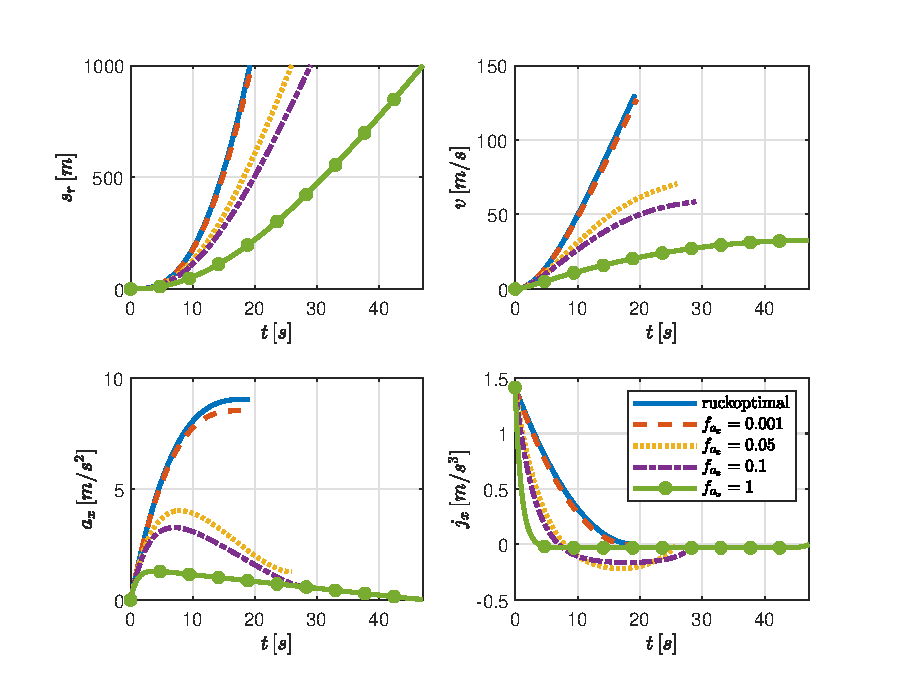
\includegraphics[width=0.8\linewidth]{./Bilder/Ergebnisse/Geradeausfahrt/var_fax.eps}
	\caption{Lösungstrajektorien der Fahrzeugzustände und der Stellgröße bei einer langen Geradeausfahrt mit $s_f=\valunit{1000}{m}$ und freien Endzuständen und freier Endzeit. Für abnehmende Bestrafung der Längsbeschleunigung nimmt die optimale Lösung immer mehr die Form der rein ruckoptimalen Lösung an. Der Ruck ist dabei mit $\fjx = 1$ gewichtet.}
	\label{fig:var_fax}
\end{figure}

\subsection{Lange Geradeausfahrt}
Ein Szenario, in dem die bisherigen Ergebnisse Anwendung finden ist die lange Geradeausfahrt, die nachfolgend eingehend analysiert werden soll. Zunächst wird die Lösung für $\fax = \fjx = 1$, also für gleiche Bestrafung von Beschleunigung und Ruck betrachtet. Das Szenario einer langen Geradeausfahrt zeichnet sich dadurch aus, dass sich der Zeitverlauf in drei Abschnitte unterteilen lässt. Im ersten Bereich für kleine Zeitpunkte gilt $0\leq t\ll t_f$, während im dritten Bereich nahe des Endzeitpunkts $0\ll t\leq t_f$ gilt. In dem Bereich dazwischen gilt $0\ll t\ll t_f$. Es zeigt sich, dass der Koeffizient des instabilen Teils $k_1$ sehr geringe Werte im Bereich von $10^{-40}\leq k_1 \leq 10^{-10}$ annimmt, wobei $k_2$ um einige Größenordnungen größer ist. Dies hat zur Folge, dass der Einfluss des instabilen Anteils erst für große $t$ (im dritten Zeitabschnitt) sichtbar wird und die Trajektorien divergieren, während das Verhalten für kleine $t$ (im ersten Zeitabschnitt) vom stabilen Teil dominiert wird und anschließend abklingt. Im Bereich dazwischen ist der Einfluss des stabilen Anteils bereits abgeklungen und der instabile Anteil ist noch nicht aufgeklungen. Folglich lässt sich die Aussage treffen, dass die Trajektorien für $t\ll t_f$ von links und für $0\ll t$ von rechts gegen den Polynomanteil konvergieren. Unter der Voraussetzung, dass die beiden Exponentialanteile jeweils nur in einem der drei Bereiche gelten, lassen sich die folgenden Annahmen treffen. Für den ersten Bereich kann der Einfluss der instabilen Mode mit $k_1(\cdot)e^{\sqrt{\frac{\fax}{\fjx}}t} \approx 0$ angenommen werden. Analog dazu gilt für den Einfluss des stabilen Anteils im dritten Bereich $k_2(\cdot)e^{-\sqrt{\frac{\fax}{\fjx}}t} \approx 0$. In diesen Bereichen gilt 
\begin{align}
j_x &\approx -k_2\sqrt{\frac{\fax}{\fjx}}e^{-\sqrt{\frac{\fax}{\fjx}}t} + \frac{c_1}{\fax} \quad\textrm{für}\quad 0\leq t\ll t_f \label{eq:j_Bereich_1} \\
a_x &\approx k_2e^{-\sqrt{\frac{\fax}{\fjx}}t} + \frac{c_1}{\fax}t - \frac{c_2}{\fax} \quad\textrm{für}\quad 0\leq t\ll t_f\,. \label{eq:a_Bereich_1}
\end{align}
sowie 
\begin{align}
j_x &\approx k_1\sqrt{\frac{\fax}{\fjx}}e^{\sqrt{\frac{\fax}{\fjx}}t} + \frac{c_1}{\fax} \quad\textrm{für}\quad 0\ll t\leq t_f \label{eq:j_Bereich_3} \\
a_x &\approx k_1e^{\sqrt{\frac{\fax}{\fjx}}t} + \frac{c_1}{\fax}t - \frac{c_2}{\fax} \quad\textrm{für}\quad 0\ll t\leq t_f\,. \label{eq:a_Bereich_3}
\end{align}
Die Trajektorien im zweiten Bereich lassen sich durch ihre Polynomanteile approximieren. Für die komfortrelevanten Größen Ruck und Beschleunigung gilt dann
\begin{align}
j_x &\approx \frac{c_1}{\fax} \quad\textrm{für}\quad 0\ll t\ll t_f \label{eq:j_Bereich_2}
\\
a_x &\approx \frac{c_1}{\fax}t - \frac{c_2}{\fax} \quad\textrm{für}\quad 0\ll t\ll t_f\,. \label{eq:a_Bereich_2}
\end{align}
Da die Trajektorien des Rucks und der Beschleunigung für lange Geradeausfahrten offenbar als Konstante bzw. Gerade betrachtet werden können, zu denen die Lösung sowohl von links als auch von rechts hin konvergiert, stellt sich die Frage, ob anhand der Kenntnis über den Lösungsraum, Beschränkungen für die Längsbeschleunigung angegeben werden können. 

\subsubsection{Begrenzung der Längsbeschleunigung}
Nachfolgend werden zwei Sets von Randbedingungen untersucht. Kenntnis über die Anfangszustände und damit Vorgabe der Anfangsbedingungen \xzero\,wird bei allen Szenarien vorausgesetzt. Allerdings kann die Vorgabe der Endwerte variiert werden. Zwei Sets an Endbedingungen erweisen sich bei der hier betrachteten langen Geradeausfahrt als besonders geeignet. Neben der Vorgabe einer Strecke $s_f$, die zurückgelegt werden soll und damit der Vorgabe des Endzustands für $s_r(t_f)$, können die Endgeschwindigkeit und -beschleunigung entweder festgelegt oder frei sein. Die Vorgabe von Endgeschwindigkeit und -beschleunigung ist sinnvoll, wenn das Fahrzeug unter Berücksichtigung des Gütefunktionals beispielsweise nach einer festgelegten Strecke unbeschleunigt zum Stehen gebracht werden soll. Wenn hingegen diese beiden Endzustände nicht festgelegt sind, weil das Ziel nur darin besteht, die vorgegebene Strecke unter Berücksichtigung des Gütefunktionals abzufahren, dann können diese Endzustände frei bleiben, wobei sich nach Gleichung \eqref{eq:Lambdaend} Endbedingungen für die adjungierten Zustände ergeben. 

\textbf{Feste Endgeschwindigkeit und feste Endbeschleunigung}

Zur Klärung der Frage, ob die Längsbeschleunigung beschränkt ist, kann eine Fallunterscheidung für die Vorzeichen der Koeffizienten $k_1$ und $k_2$ vorgenommen werden. So lässt sich feststellen, dass der stabile und instabile Anteil in Gleichung \eqref{eq:DGL_ax_Lösung} bei identischem Vorzeichen die gleiche Krümmungsrichtung haben (unabhängig davon, ob das Vorzeichen positiv oder negativ ist). Das bedeutet, dass die Exponentialanteile entweder beide von oben oder beide von unten gegen den linearen Lösungsanteil konvergieren. Für die Lösung des Rucks bedeuten identische Vorzeichen, dass die Krümmungen der Exponentialanteile in der Lösung in Gleichung \eqref{eq:DGL_jx_Lösung} immer entgegengesetzte Richtungen haben und einer der Anteile von oben gegen die Konstante konvergiert, während der andere Teil von unten gegen die Konstante läuft. Aufgrund des streng monotonen Verhaltens der Exponentialfunktionen, ist auch der Ruck über das gesamte Lösungsintervall streng monoton, sodass $j_x$ genau eine Nullstelle hat\footnote{Streng genommen muss diese Nullstelle nicht zwangsläufig innerhalb des Lösungsintervalls liegen.}. Dadurch, dass der Ruck genau eine Nullstelle besitzt, hat $a_x$ genau ein Extremum. Mit der Kenntnis, dass die Beschleunigung ausgehend vom Anfangswert $a_0$ gegen die Gerade in Bereich zwei konvergiert und anschließend unter Beibehaltung der Krümmungrichtung von der Geraden weg gegen den Endwert $a_f$ läuft, lasst sich feststellen, dass die Beschleunigung bei gleichem Vorzeichen der Koeffizienten $k_1$ und $k_2$ stets durch den linearen Anteil der Lösung und die Verbindungsgerade zwischen $a_0$ und $a_f$ beschränkt ist. In Abbildung \ref{fig:vf_af_fest_gleiches_VZ} sind die optimalen Lösungstrajektorien der Fahrzeugzustände $s_r$, $v$ und $a_x$ sowie der Stellgröße $j_x$ bei vorgegebenen Endzuständen und ansonsten identischer Parametrierung dargestellt. Die Anfangsgeschwindigkeit wurde so gewählt, dass die Vorzeichen der Lösungen von $k_1$ und $k_2$ identisch sind. Die Endzustände wurden so gewählt, dass das Fahrzeug nach \valunit{1000}{m} unbeschleunigt zum Stehen kommt. Der Endzeitpunkt wurde im Sinne einer einheitlichen Darstellung fest zu $t_f = \valunit{40}{s}$ gewählt. Das zuvor beschriebene Verhalten der Beschleunigungs- und Rucktrajektorien ist gut in den unteren beiden Graphen zu erkennen. Zum einen lassen sich die beiden Bereiche erkennen, in denen die Lösungen von den Exponentialteilen dominiert werden, sowie der mittlere Bereiche, in dem die Lösungen der Geraden für die Beschleunigung und der Konstanten für den Ruck entsprechen. Zudem zeigt die Abbildung unten links die Beschränkung der Beschleunigung (grau schattiert) durch die Verbindungsgerade der Randwerte und den linearen Anteil der Lösung.
\begin{figure}[h] 
	\centering
	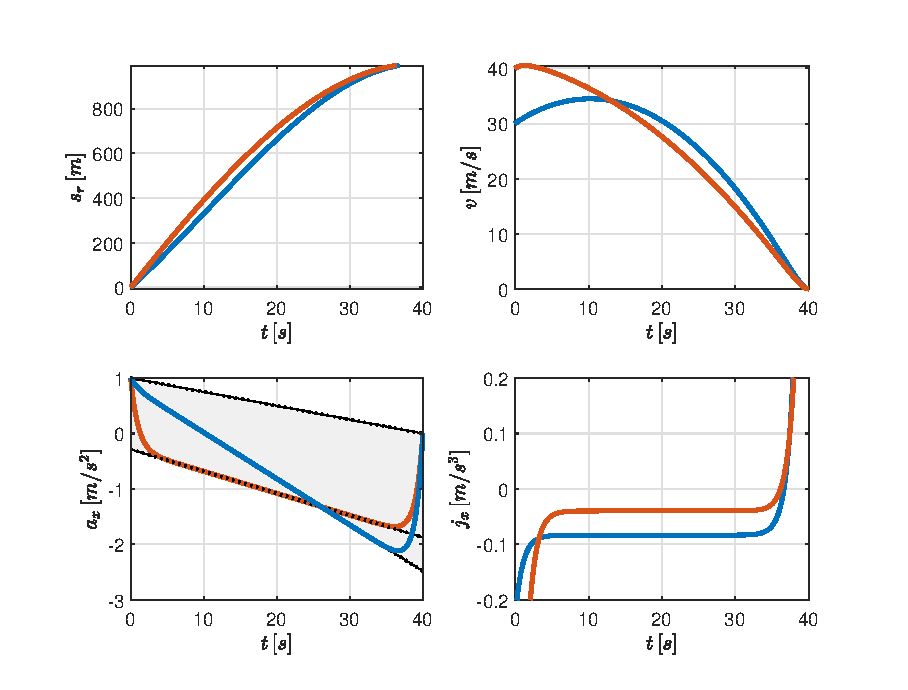
\includegraphics[width=\linewidth]{./Bilder/Ergebnisse/Geradeausfahrt/vf_af_fest_gleiches_VZ.eps}
	\caption{Lösungstrajektorien der Fahrzeugzustände und der Stellgröße bei einer langen Geradeausfahrt mit $s_f=\valunit{1000}{m}$ und fester Endgeschwindigkeit und -beschleunigung. Das Vorzeichen von $k_1$ und $k_2$ ist identisch.}
	\label{fig:vf_af_fest_gleiches_VZ}
\end{figure}

Für den Fall, dass das Vorzeichen der Koeffizenten $k_1$ und $k_2$ unterschiedlich ist, haben die Exponentialanteile in $j_x$ dieselbe Krümmungsrichtung und laufen damit beide entweder von oben oder von unten gegen die Konstante, während die Anteile in $a_x$ mit unterschiedlichen Vorzeichen wirken. Damit lässt sich feststellen, dass $j_x$ immer zwei Nullstellen besitzt, weshalb in $a_x$ zwei Extrema auftreten können. Da $j_x$ bei zwei Nullstellen einen Vorzeichenwechsel aufweist, hat die Steigung der Beschleunigung einen Richtungswechsel, woraus abgeleitet werden kann, dass es bei zwei Extrema ein Maximum und ein Minimum gibt und die Lösung von $a_x$ die Verbindungsgerade der Randwerte in einem Punkt schneidet. Dadurch, dass die Exponentialanteile der Lösung auch hier wieder gegen den linearen Anteil konvergieren, kann schließlich auch in diesem Fall argumentiert werden, dass die Beschleunigung stets durch die Verbindungsgerade von $a_0$ und $a_f$ und den linearen Anteil beschränkt ist, wobei sich die Geraden im mittleren Abschnitt bei 
\begin{equation}
t = \frac{a_0\fax + c_2}{c_1 - \frac{\fax(a_f - a_0)}{t_f}}
\end{equation} 
schneiden. Das Verhalten für diesen Lösungsfall ist in Abbildung \ref{fig:vf_af_fest_unterschiedliches_VZ} dargestellt. In den Graphen der Beschleunigung und des Rucks zeigt sich deutlich das beschriebene Verhalten mit den unterschiedlich gekrümmten Exponentialanteilen sowie die Konvergenz von links und rechts hin zu der jeweiligen Lösung auf dem mittleren Abschnitt. Außerdem ist die Beschränkung der Beschleunigung gut zu erkennen. 
\begin{figure}[h] 
	\centering
	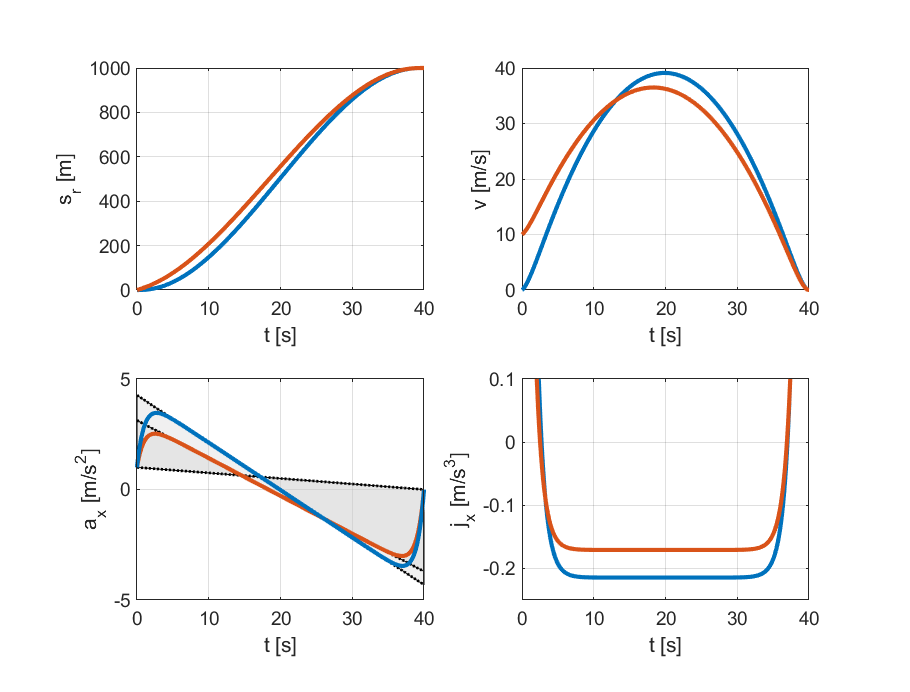
\includegraphics[width=\linewidth]{./Bilder/Ergebnisse/Geradeausfahrt/vf_af_fest_unterschiedliches_VZ.eps}
	\caption{Lösungstrajektorien der Fahrzeugzustände und der Stellgröße bei einer langen Geradeausfahrt mit $s_f=\valunit{1000}{m}$ und fester Endgeschwindigkeit und -beschleunigung. Das Vorzeichen von $k_1$ und $k_2$ ist unterschiedlich.}
	\label{fig:vf_af_fest_unterschiedliches_VZ}
\end{figure}

\textbf{Freie Endgeschwindigkeit und freie Endbeschleunigung}

Dadurch, dass die Endzustände $v(t_f)$ und $a_x(t_f)$ nicht festgelegt sind, ergeben sich die Endbedingungen $\lambda_2(t_f) = 0$ und $\lambda_3(t_f) = 0 \rightarrow j_x(t_f) = 0$. Bei dieser Wahl der Endbedingungen ist die analytische Herleitung der maximalen und minimalen Beschleunigung möglich, welche nachfolgend betrachtet werden soll.. Da $j_x$ bis auf die beiden Exponentialanteile konstant ist, kann argumentiert werden, dass der Ruck maximal zwei Nullstellen aufweist, wobei diese nicht in Bereich zwei liegen können (in diesem Bereich ist $j_x$ näherungsweise konstant). Ein Kontinuum an Nullstellen in Bereich zwei ist aufgrund des monotonen Verhaltens der Exponentialfunktionen nicht möglich, weshalb der Ruck im ersten und im dritten Bereich auf Nullstellen untersucht wird. Im ersten Bereich folgt mit $j_x \stackrel{!}{=} 0$ aus Gleichung \eqref{eq:j_Bereich_1}
\begin{equation}
	t_{z,1} = -\sqrt{\frac{\fjx}{\fax}}\ln{\Big(\frac{c_1}{k_2}\sqrt{\frac{\fjx}{\fax^3}}\Big)}\,. \label{eq:t_z_1}
\end{equation}
Dadurch, dass die Endgeschwindigkeit frei ist, ergibt sich die Endbedingung 
\begin{equation}
	\lambda_2(t_f) = -c_1t_f + c_2 \stackrel{!}{=} 0\,.
\end{equation}
Mit der Anfangsbedingung für die Beschleunigung $a_x(0) = a_0$ folgt aus Gleichung \eqref{eq:a_Bereich_1}
\begin{equation}
k_2 = a_0 + \frac{c_2}{\fax} = a_0 + \frac{c_1t_f}{\fax}\,.
\end{equation}
Wird dieser Zusammenhang in Gleichung \eqref{eq:t_z_1} eingesetzt, erhält man mit 
\begin{equation}
t_{z,1} = -\sqrt{\frac{\fjx}{\fax}}\ln{\Big(\frac{c_1}{a_0+\frac{c_1t_f}{\fax}}\sqrt{\frac{\fjx}{\fax^3}}\Big)}
\end{equation}
den Zeitpunkt des Nulldurchgang von $j_x$ im ersten Bereich, wobei dieser vom Anfangswert der Beschleunigung, den Gewichtungsfaktoren der Komfortkriterien, dem Endzeitpunkt und der Lösung von $\lambda_1$ abhängt. Einsetzen von $t_{z,1}$ in Gleichung \eqref{eq:a_Bereich_1} liefert den Extremwert der Beschleunigung an dieser Stelle mit 
\begin{equation}
a_{x_{z,1}} = c_1\sqrt{\frac{\fjx}{\fax^3}} -c_1\sqrt{\frac{\fjx}{\fax^3}}\ln{\Big(\frac{c_1}{a_0+\frac{c_1t_f}{\fax}}\sqrt{\frac{\fjx}{\fax^3}}\Big)} - \frac{c_1t_f}{\fax}\,. 
\end{equation}
Die zweite Nullstelle von $j_x$ resultiert in dieser Wahl der Randbedingungen direkt aus $j_x(t_f) = 0$. Der Ruck hat folglich immer bei $t_{z,2} = t_f$ ein Extremum. Aus Gleichung \eqref{eq:j_Bereich_3} folgt 
\begin{equation}
k_1 = -\frac{c_1\sqrt{\frac{\fjx}{\fax^3}}}{e^{\sqrt{\frac{\fax}{\fjx}}t_f}}\,.
\end{equation}
Eingesetzt in Gleichung \eqref{eq:a_Bereich_3} lautet die Beschleunigung der zweiten Extremstelle
\begin{equation}
a_{x_{z,2}} = -c_1\sqrt{\frac{\fjx}{\fax^3}} + \frac{c_1}{\fax}t_f - \frac{c_1t_f}{\fax} = -c_1\sqrt{\frac{\fjx}{\fax^3}}\,. 
\end{equation}
Es lässt sich also festhalten, dass bei freien Endzuständen eine Extremstelle der Beschleunigung bei $t_f$ liegt und eine im ersten Abschnitt. Da der Endwert der Beschleunigung bei positiver Steigung immer unter dem linearen Lösungsanteil und bei negativer Steigung oberhalb der Geraden liegt, ist die Beschränkung durch den linearen Anteil der Lösung streng genommen nicht mehr gültig. Dennoch ist die Gerade als Näherungslösung für die Beschränkung geeignet wie Abbildung \ref{fig:vf_af_frei} zeigt. In der Abbildung sind die optimalen Zustands- und Stellgrößentrajektorien für unterschiedliche Anfangsgeschwindigkeiten gezeigt, sodass der Ruck und die Beschleunigung jeweils einmal von unten und von oben gegen die Approximation in Bereich zwei konvergieren. Der kleine Ausschhnitt in der Mitte der Abbildung gehört zum Graph der Beschleunigung unten links und zeigt den vergrößerten Abschnitt im Bereich von \valunit{36}{s} bis \valunit{40}{s}. Dabei wird deutlich, dass der Endwert der Beschleunigung jeweils außerhalb der durch die Verbindungsgerade und den linearen Anteil der Beschleunigungstrajektorie eingeschlossenen Fläche liegt und damit streng genommen außerhalb der Beschränkung. Da diese Verfehlung allerdings nur einen geringen Einfluss hat, lässt sich der lineare Anteil trotzdem zumindest als Näherungslösung für die Beschränkung verwenden. Zudem zeigt die Abbildung die beiden Nullstellen von $j_x$ und damit Extremstellen von $a_x$, von denen eine jeweils bei $t_f$ liegt.
\begin{figure}[h] 
	\centering
	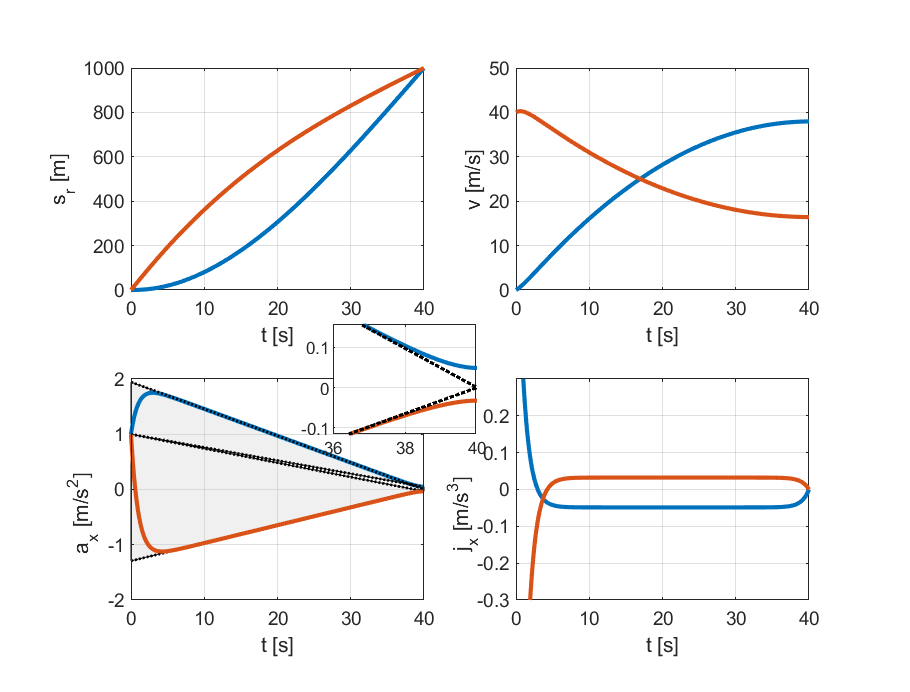
\includegraphics[width=\linewidth]{./Bilder/Ergebnisse/Geradeausfahrt/vf_af_frei_mit_zoom_aspectratio.eps}
	\caption{Lösungstrajektorien der Fahrzeugzustände und der Stellgröße bei einer langen Geradeausfahrt mit $s_f=\valunit{1000}{m}$ und freier Endgeschwindigkeit und -beschleunigung.}
	\label{fig:vf_af_frei}
\end{figure} 

Abschließend lässt sich festhalten, dass die analytischen Lösungen der optimalen Trajektorien für die Geradeausfahrt sowohl für ein rein energieoptimales Gütefunktional als auch für ein Gütefunktional mit zusätzlicher Bestrafung der Längsbeschleunigung bestimmt werden können und die verbleibenden Unbekannten mithilfe der Randbedingungen des Optimierungsproblems durch Lösung eines nichtlinearen Gleichungssystems berechnet werden können. Außerdem lässt sich unter Zuhilfenahme einiger Annahmen eine Abschätzung für die Beschränkung der Längsbeschleunigung treffen, über die wiederum Aussagen über den erwarteten Fahrkomfort getroffen werden können. Während der Anfangswert des Längsrucks nicht vorgegeben werden kann, sodass unter Umständen hohe Ruckwerte zu Beginn auftreten können, lässt sich der Endwert des Rucks bei freier Endbeschleunigung über die Endbedingung $\lambda_3(t_f) = 0$ vorgeben. 

\subsection{Heranfahren an eine Ampel bei bekannter Rotphase}\label{subsec:Ampelszenario}
Die Erkenntnisse über den Lösungsraum bei einer Geradeausfahrt mit beschleunigungs- und ruckoptimalem Gütefunktional werden nachfolgend verwendet, um das Heranfahren an eine Ampel mit bekannter Rotphase zu analysieren. Neben der Analyse des Anhalte- bzw. Anfahrvorgangs unter dem Aspekt des Fahrkomforts, dient dieses Szenario auch dem Vergleich zwischen vorausschauender Planung über die Ampelüberquerung hinaus und der weniger vorausschauenden zwei geteilten Planung bis zur Ampel und von dort aus bis zum Zielpunkt. Letzteres entspricht dabei dem vom Menschen gewählten Planungsverhalten, wobei die vorausschauende Variante einige Vorteile bietet. 

Das beschriebene Szenario kann als Geradeausfahrt interpretiert werden, bei der sich das Fahrzeug zu einem bestimmten Zeitpunkt $t_1$ an der Ampel befinden soll. Der Ort, an dem sich die Ampel befindet, kann dabei als die vom Startpunkt der Optimierung aus zurückzulegende Strecke $s_1$ betrachtet werden. Damit ein solches Szenario realistisch umsetzbar ist, muss die Strecke $s_1$ vom Fahrzeug bis zur Ampel, sowie der Zeitpunkt $t_1$ bekannt sein. Dieser wird als der Moment interpretiert, in dem die Ampel von rot auf grün springt und damit das Überqueren der Ampel für das Fahrzeug erlaubt ist\footnote{Ein Ansatz wie der Verkehrsfluss mithilfe von Fahrzeug zu Ampel Kommunikation und adaptiver Ampelphasen in Abhängigkeit des Verkehrsaufkommens verbessert werden kann, wurde in \cite{Gradinescu} untersucht.}. Das Szenario lässt sich dann mithilfe der internen \gls{GNB} $s_r(t_1) = s_1$ bei festem und bekanntem $t_1$ beschreiben. Alternativ kann das Szenario als zwei zusammengesetzte Geradenabschnitte verstanden werden, die an dem über die Zeit und die Strecke definierten Punkt $\mathcal{P}_1 = (t_1, s_1)$ miteinander verknüpft sind. Die Systemdynamik bleibt in den beiden Zeitabschnitten unverändert. Wird die insgesamt benötigte Zeit $t_f$ als Komfortkriterium verwendet, um möglichst schnell zum Zielort zu gelangen, dann kann das Szenario als ein Gesamtoptimierungsproblem mit der internen \gls{GNB} betrachtet werden, wobei $t_f$ über das gesamte Szenario bei der Optimierung berücksichtigt wird. Stattdessen kann das Szenario auch als zwei seperate Optimierungsprobleme formuliert werden, wobei das zweite Optimierungsproblem auf dem ersten aufsetzt, während bei den beiden Problemformulierungen nur das Verhalten im jeweiligen Zeitabschnitt $t_0 \leq t \leq t_1$ bzw. $t_1 \leq t \leq t_f$ berücksichtigt wird. Es sei an dieser Stelle darauf hingewiesen, dass die beiden Herangehensweisen das Problem zu formulieren nicht äquivalent sind und nicht zu erwarten ist, dass sie identische Ergebnisse liefern. Sie dienen aber der Unterscheidung zwischen dem erwarteten menschlichen Verhalten und dem maschinellen Verhalten eines automatisierten Fahrzeugs, was durch eine einfache Optimierung mit Blick auf das Gesamtintervall erreicht werden kann.

\subsubsection{Vorausschauende Planung}\label{subsubsec:Vorausschauend}
Zunächst soll die vorausschauende Planung des Heranfahrens an die Ampel untersucht werden. Das Optimierungsproblem für dieses Szenario kann wie folgt formuliert werden
\begin{align}
\min_{\ve{u}} \quad & J(\ve{x},\ve{u},t,t_f) = t_f + \int_{t_0}^{t_f}\frac{1}{2}\fjx j_x^2 + \frac{1}{2}\fax a_x^2\dtint{t} \\
\textrm{u.B.v.} \quad& \xoftzero = \xzero \\
& s_r(t_1) = s_1 \label{eq:srt1_gleich_s1}\\
& s_r(t_f ) = s_f\,,
\end{align}
wobei die Endzeit frei ist und als Optimierungsvariable betrachtet wird, während der Zeitpunkt $t_1$, zu dem die Ampel überquert werden soll, als fest betrachtet wird. Bis auf die festgelegte Zielstrecke $s_f$ sind die Endzustände frei. Das Ziel dieser Optimierung ist demnach, die Strecke $s_f$ möglichst schnell zurückzulegen unter Berücksichtigung der bekannten Ampelphase und des Fahrkomforts. Während die Beschreibung der Systemdynamik nicht verändert wird, stellt Gleichung \eqref{eq:srt1_gleich_s1} eine interne \gls{GNB} dar. Die Forderung nach Stetigkeit der Fahrzeugzustände im Übergangspunkt $\mathcal{P}_1$ führt zur Stetigkeitsbedingung 
\begin{equation}
\xoftoneminus = \xoftoneplus
\end{equation}
und schließlich zu der ersten Weierstrass-Erdmannschen-Eckenbedingung (siehe Kapitel \ref{sec:InterneGNB})
\begin{align}
2\tilde{\nu} - \lambda_1(t_1^-) + \lambda_1(t_1^+) &= 0\\
\lambda_2(t_1^-) + \lambda_2(t_1^+) &= 0\\
\lambda_3(t_1^-) + \lambda_3(t_1^+) &= 0\,. \label{eq:l3tminus_l3tplus}
\end{align}
Da $t_1$ fest ist, fällt die zweite Weierstrass-Erdmannschen-Eckenbedingung weg. Im Gegensatz zum menschlichen Planungsverhalten wird die vorausschauende Planung durch die Tatsache definiert, dass das Überqueren der Ampel am Punkt $\mathcal{P}_1$ über eine \gls{GNB} berücksichtigt wird, während die Gesamtzeit $t_f$ bei der Optimierung berücksichtigt wird.

\subsubsection{Menschliche Planung}\label{subsubsec:Mensch}
Bei der menschlichen Planung hingegen lässt sich das Optimierungsproblem, welches das selbe Gesamtziel hat - die Strecke $s_f$ unter Berücksichtigung der Ampelphase möglichst schnell zurückzulegen - in zwei Teilprobleme unterteilen. Für das Gesamtproblem gilt
\begin{equation}
\min_{\ve{u}} \, J(\ve{x},\ve{u},t,t_f) = \min_{\ve{u}} \, J_1(\ve{x},\ve{u},t,t_1) + \min_{\ve{u}} \, J_2(\ve{x},\ve{u},t,t_2)\,.
\end{equation}
Die Teilprobleme $J_1$ und $J_2$ lassen sich dabei wie folgt formulieren
\begin{multicols}{2}
	\begin{align}
	J_1(\ve{x},\ve{u},t,t_1) &= t_1 + \int_{t_0}^{t_1}\frac{1}{2}\fjx j_x^2 + \frac{1}{2}\fax a_x^2\dtint{t} \\
	\textrm{u.B.v.} \quad \xoftzero &= \xzero \\
	s_r(t_1) &= s_1 
	\end{align}
	\columnbreak
	\begin{align}
	J_2(\ve{x},\ve{u},t,t_f) &= (t_f - t_1) + \int_{t_1}^{t_f}\frac{1}{2}\fjx j_x^2 + \frac{1}{2}\fax a_x^2\dtint{t} \\
	\textrm{u.B.v.} \quad \xoftone &= \ve{x}_1 \\
	s_r(t_f) &= s_f 
	\end{align}
\end{multicols}
Diese lassen sich getrennt voneinander lösen und anschließend zur Lösung des Gesamtproblems zusammensetzen. Die Gesamtzeit wird in dieser Art der Problemformulierung also dadurch berücksichtigt, dass die Zeiten der beiden Teilprobleme optimiert werden, wobei das Fahrzeugverhalten für $t>t_1$ im ersten Teilproblem nicht berücksichtigt werden kann und umgekehrt. Der Anfangszustand $\ve{x}_1$ des zweiten Teilproblems entspricht der Lösung des ersten Teilproblems zum Zeitpunkt $t_1$.

\subsubsection{Vergleich der Planungsstrategien}\label{subsubsec:Vergleich}
In Abbildung \ref{fig:svaj_zoomj} sind die optimalen Trajektorien für die beiden erläuterten Planungsstrategien für zwei unterschiedliche Anfangsgeschwindigkeiten dargestellt. In den dargestellten Fällen wurde die Gewichtung $\fax = 1$ und $\fjx = 1$ gewählt. Außerdem wurden der Ort und die Zeit, zu denen die Ampel überquert werden soll, zu $\mathcal{P}_1 = (\valunit{40}{s}, \valunit{350}{m})$ gewählt. Die Gesamtstrecke beträgt $s_f = \valunit{600}{m}$. Wird zunächst nur das Verhalten der vorausschauenden Planung betrachtet (durchgezogene Linien), so fällt ein Unterschied im Beschleunigungsverhalten bzw. im Geschwindigkeitsprofil auf. Startet das Fahrzeug mit einer niedrigen Geschwindigkeit ($v_0 = \valunit{5}{\frac{\unit{m}}{\unit{s}}}$, blaue Linie), beginnt das Fahrzeug sofort zu beschleunigen und die Geschwindigkeit zu erhöhen und überquert die Ampel mit $v(t_1) = \valunit{16{,}78}{\frac{\unit{m}}{\unit{s}}}$. Für den Fall, dass das Fahrzeug bereits mit einer vergleichsweise hohen Geschwindigkeit startet ($v_0 = \valunit{15}{\frac{\unit{m}}{\unit{s}}}$, rote Linie), muss die Geschwindigkeit zunächst gedrosselt werden, damit die Ampel nicht zu früh überquert und damit die Rotphase der Ampel gerissen wird. Die Ampel wird in diesem Fall bei $\mathcal{P}_1$ mit $v(t_1) = \valunit{13{,}02}{\frac{\unit{m}}{\unit{s}}}$, also mit geringerer Geschwindigkeit, passiert. Beim Beschleunigungsverhalten zeigt sich, dass der Betrag der Trajektorie bei einer niedrigeren Startgeschwindigkeit geringere Werte annimmt und daher komfortabler ist im Vergleich zum Starten mit hoher Anfangsgeschwindigkeit. Die niedrigere Startgeschwindigkeit erreicht jedoch nicht nur aus Sicht der Beschleunigung ein höheres Maß an Fahrkomfort. Gleichzeitig lässt sich das Planungsziel schneller erreichen, da das anfängliche Abbremsen nicht notwendig ist und stattdessen von Beginn an gleichmäßig beschleunigt werden kann. In beiden Fällen lässt sich zudem aufgrund der Bedingung \eqref{eq:l3tminus_l3tplus} Stetigkeit für $j_x$ erreichen und so insgesamt ruckarme Lösungen erzielen. Betrachtet man nun die Lösungen bei der menschlichen Planung (gestrichelte Linien), lassen sich die selben qualitativen Zusammenhänge erkennen. Auch bei dieser Art der Planung ist es günstiger mit einer geringeren Geschwindigkeit zu starten, da sich das Ziel dadurch schneller erreichen lässt und geringere Beschleunigungen benötigt werden. Vor allem fällt jedoch auf, dass aufgrund der zweifachen Planungen, die bis auf den Anfangszustand unabhängig voneinander sind, in beiden Abschnitten der Anfangsruck nicht vorgegeben werden kann, sodass der Ruck unstetig ist und bei $\mathcal{P}_1$ eine Sprungstelle auftritt. Diese Sprungstelle führt zu deutlich größeren Ruckwerten als bei der vorausschauenden Planung. In \ref{Anhang} ist nochmals der Plot der Stellgröße dargestellt, allerdings mit einer weiteren Achsenskalierung, sodass die kompletten Ruckverläufe inklusive der Überhöhungen an der Sprungstelle zu erkennen sind. Neben den weniger komfortablen Rucktrajektorien, zeigt das Geschwindigkeitsprofil einen weiteren Nachteil der menschlichen Planung gegenüber der vorausschauenden Planung. Das menschliche Verhalten in der weniger vorausschauenden Planung wird damit begründet, dass die Planung abschnittsweise vom Startpunkt bis zur Ampel und von dort bis zum Zielpunkt stattfindet, ohne dass der Abschnitt nach der Ampel im ersten Abschnitt berücksichtigt wird. Dies hat zur Folge, dass die Geschwindigkeit $v(t_1)$ an der Ampel geringer ist, als sie im Idealfall bei vorausschauender Planung sein könnte, weshalb das Fahrzeug bei menschliche Planung immer mehr Zeit benötigt.
\begin{figure}[h] 
	\centering
	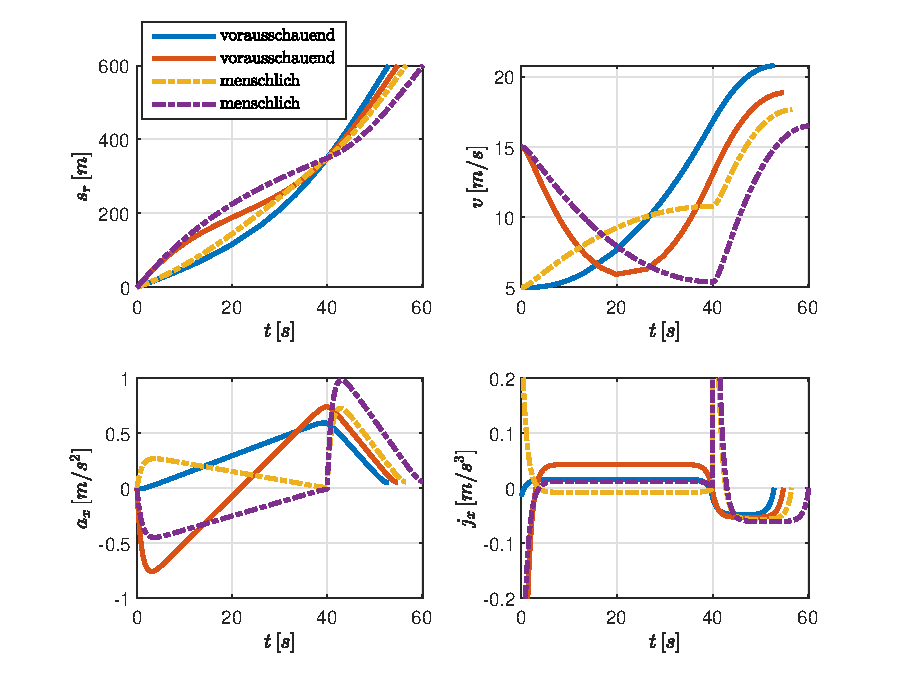
\includegraphics[width=\linewidth]{./Bilder/Ergebnisse/Geradeausfahrt/Ampel/v_5_v_15/svaj_zoomj.eps}
	\caption{Lösungstrajektorien der Fahrzeugzustände und der Stellgröße beim Zufahren auf eine Ampel mit bekannter Rotphase. Darstellung der Ergebnisse für vorausschauende und menschliche (weniger vorausschauend) Planung bei unterschiedlichen Startgeschwindigkeiten.}
	\label{fig:svaj_zoomj}
\end{figure} 

\textbf{Idealer Bremsvorgang}

Als Abschluss dieses Szenarios soll der Blick nochmal speziell auf den Bremsvorgang vor der Ampel bei hohen Anfangsgeschwindigkeiten gerichtet werden. Dazu sind in Abbildung \ref{fig:va_fa_variabel} die Geschwindigkeits- und Beschleunigungsverläufe von vorausschauender und menschlicher Planung für das Szenario mit der höheren Anfangsgeschwindigkeit gezeigt, allerdings mit unterschiedlichen Gewichtungen \fax\,der Beschleunigung. Dabei zeigt sich, dass die Geschwindigkeit an der Ampel am geringsten ist. Dieses Verhalten entspricht dabei am ehesten dem, wie sich eine fahrende Person im Straßenverkehr verhalten würde - man würde so lange die Geschwindigkeit reduzieren, bis die Ampel schließlich wieder auf grün springt. Bei der vorausschauenden Planung hingegen wird das Minimum deutlich früher erreicht. Dies mag auf den ersten Blick nicht gerade intuitiv erscheinen, da es bedeutet, dass schon stark verzögert wird, obwohl das Fahrzeug noch weit von der Ampel entfernt ist. Zudem bedeutet es, dass bereits beschleunigt wird, bevor die Ampel grün zeigt. Durch diese Weitsicht kann die Ampel allerdings mit höherer Geschwindigkeit überquert und das Endziel schneller erreicht werden. Die vorausschauende Planung mag zwar aus Sicht der Komfortkriterien besser abschneiden, als die menschliche Planung, allerdings ist sie nicht in allen Verkehrssituationen praktikabel. Bei besonders hohem Verkehrsaufkommen, bei dem sich der Verkehr möglicherweise vor einer Ampel staut, ist diese Art der Planung nicht sinnvoll nutzbar, da das Fahrzeug vor der Ampel keine freie Fahrt hat und dadurch nicht schon weit vor der Ampel beschleunigen kann, wie es von der Trajektorie verlangt wird. Zudem würde das starke Abbremsen weit vor der Ampel dazu führen, dass der nachfolgende Verkehr ausgebremst wird.
\begin{figure}[h] 
	\centering
	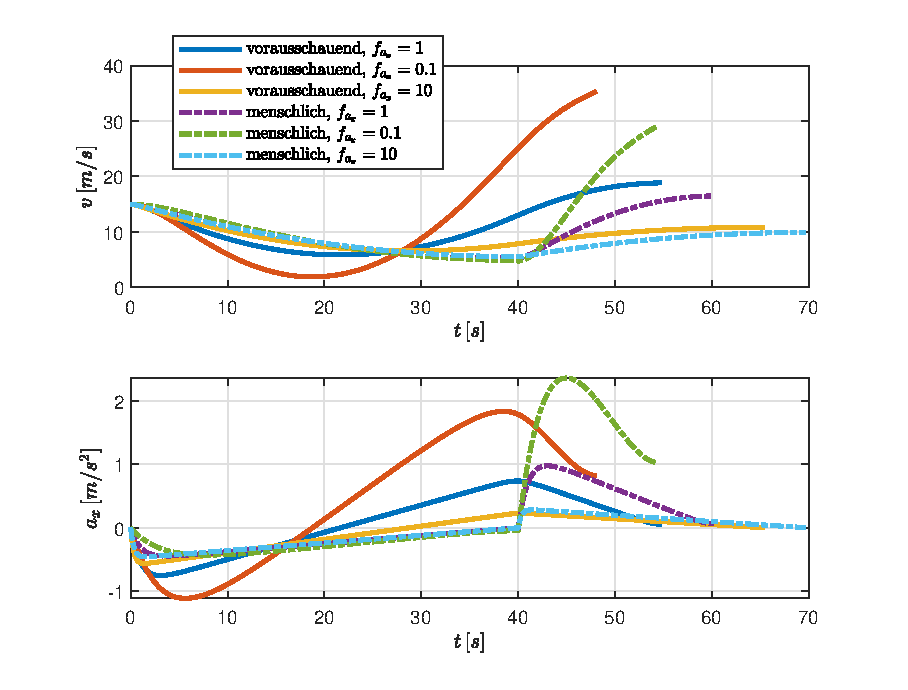
\includegraphics[width=0.9\linewidth]{./Bilder/Ergebnisse/Geradeausfahrt/Ampel/v_5_v_15/va_fa_variabel.eps}
	\caption{Geschwindigkeits- und Beschleunigungstrajektorien für vorausschauende und menschliche Planung für unterschiedliche Gewichtungen der Beschleunigung bei höherer Startgeschwindigkeit.}
	\label{fig:va_fa_variabel}
\end{figure} 
 

\section{Spurwechsel}\label{sec:Spurwechsel}
Bisher wurde ausschließlich die Längsdynamik des Fahrzeugs bei den untersuchten Szenarien berücksichtigt. Das nachfolgend untersuchte Szenario Spurwechsel stellt insofern eine Erweiterung der bisher betrachteten Szenarien dar, als dass nun unter Hinzunahme der querdynamischen Größen das Gesamtmodell des Fahrzeugs verwendet wird. Dadurch lassen sich Spurwechsel beschreiben und hinsichtlich der Querdynamik analysieren. 

\subsection{Komfortgewinn durch variable Gewichtung der Querabweichung}
\section{Kreisfahrt mit konstanter Krümmung}
Nachdem das Szenario Geradeausfahrt eingehend analysiert und diskutiert wurde, soll nachfolgend das Szenario einer Kreisfahrt untersucht werden. Die Kreisfahrt stellt mit seiner konstanten Krümmung einen vereinfachten Sonderfall einer Kurve dar. Durch die Analyse der Kreisfahrt lassen sich einige Erkenntnisse gewinnen, die später bei der Untersuchung allgemeiner Kurven mit veränderlicher Krümmung, sogenannter Klothoiden, wieder auftauchen.

\subsection{Vernachlässigung der Querdynamik}
\subsubsection{Ruhelage}
\subsection{Berücksichtung der Querdynamik}
\subsubsection{Ruhelage}
\section{Klothoide mit konstanter Krümmungsänderung}
\section{Gerade-Kurvenkombination}
\section{Rundkurs}


% =================================================================================
% Anhang
% =================================================================================
\appendix % Damit wird der Anhang begonnen. Die Kapitel werden ab jetzt mit Buchstaben nummeriert


% =================================================================================
% Literaturverzeichnis
% =================================================================================
\cleardoublepage        % Auf eine leere Seite einfügen
\phantomsection         % Für Aufnahme ins Inhaltsverzeichnis
\addcontentsline{toc}{chapter}{\bibname}  % In Inhaltsverzeichnis von
                                          % Dokument und pdf aufnehmen
\printbibliography 
% =================================================================================

	
\end{document}
